\documentclass[a4paper,10pt]{article}
%\documentclass[a4paper,10pt]{report} for proposal
\usepackage[T1]{fontenc}
\usepackage[latin9]{inputenc}
%\usepackage[utf8]{inputenc}
%\usepackage{graphicx}
%\usepackage{epstopdf}
\usepackage{array}
\usepackage{times}
 \usepackage[pdftex]{hyperref}
%\usepackage[pdftex]{graphicx}
%\usepackage[dvips]{graphicx}
\usepackage{graphicx,epstopdf}
\epstopdfsetup{suffix=}
\DeclareGraphicsExtensions{.ps}
\DeclareGraphicsRule{.ps}{pdf}{.pdf}{`ps2pdf -dEPSCrop -dNOSAFER #1 \noexpand\OutputFile}
\usepackage{float}
\usepackage{amsfonts}
\usepackage[affil-it]{authblk}
\usepackage{amsthm}
\usepackage{amsmath}
\usepackage{amssymb}
\usepackage{color}
\usepackage{tikz}
\usepackage{subcaption}
\usepackage[export]{adjustbox}
\usepackage{wrapfig}
\usepackage{multirow}
\textwidth 16.5truecm \textheight 20truecm \hoffset -2.2truecm
\numberwithin{equation}{section}
\renewcommand{\thesubfigure}{\Alph{subfigure}}
%\usepackage[backend=bibtex,
%style=numeric,
%bibencoding=ascii,
%%style=alphabetic
%%style=reading
%sorting=ynt
%]{biblatex}
\usepackage[english]{babel}
\usepackage[nottoc]{tocbibind}
\usepackage[numbers,sort]{natbib}
\usepackage{textcomp,gensymb}
\bibliographystyle{abbrvnat}



%\addbibresource{review.bib}
\title{A uniform mechanism designed for the cyanobacterial circadian oscillator reveals convergent evolution}

\author{Yining Lu}
\author{Daniel Forger}
\affil{Department of Mathematics,\\University of Michigan}


\date{}
\begin{document}

\maketitle

%\tableofcontents
\begin{abstract}
Circadian clocks are vital systems in many organisms, among which cyanobacteria has the simplest clock with KaiC phosphorylation as the pacemaker. Three clock proteins KaiA, KaiB, and KaiC, and their interactions have been studied extensively. We first present a detailed  mechanism for the circadian clock system. Our model is able to reproduce important experimental results including temperature compensation and robustness under ATP variations. Predictions are also proposed in terms of conditions for sustaining oscillations. Despite the huge difference in mammal and cyanobacteria, our mathematical analysis on a simplified model shows that the core mechanism in the cyanobacterial circadian clock shares similar features as the mammalian clock, revealing convergent evolution on a high level. Sequestration of the activator through tight binding and a stoichiometric condition are vital in synchronizing the molecules as well as sustaining the rhythm. 
\end{abstract}

\section{Introduction}
Endogenous circadian clocks are self-sustained biological oscillators present in many species, the period of which are roughly 24 hours. This rhythmic behavior is vital in order for organisms to have reliable regulations of biological activities. Cyanobacteria are the simplest organisms in which a stable circadian rhythm can be found. It has been discovered that there are three key clock proteins in Cyanobacteria, KaiA, KaiB and KaiC~\citet{ishi1998}. Although it was widely accepted that the main drive for circadian rhythms in higher organisms is the negative feedback loop regulating gene expression, early experiments in  \citet{johnson2000} show that even when metabolic activity including total RNA and protein synthesis in cyanobacteria \textit{Synechococcus elongatus} is suppressed under constant dark condition (DD) for a few days, the circadian rhythm does not reset, suggesting the possibility that the cyanobacterial central clock  continues to oscillate in DD. A ground breaking result follows in \citet{Tamito2005} with clear evidence of temperature-compensated, robust circadian rhythms of
KaiC phosphorylation without transcription or translation. They also find that KaiC \textit{in vitro} autokainase/autophosphatase activity is robust to temperature changes. Even more exciting results were found in   \citet{nakajima2005} where self-sustainable oscillation of KaiC phosphorylation can be  reconstituted in
vitro by incubating KaiC with KaiA, KaiB and ATP. \citet{Tamito2005} have shown in their pioneering work that sustained circadian rhythm in phosphorylation can occur \textit{in vivo} without any transcription-translation feedback loops. Moreover, \citet{nakajima2005}	reconstructed \textit{in vitro} the robust circadian oscillation with only ATP and the three clock Kai-proteins.
The oscillation constructed \textit{in vitro} therein is temperature compensated with a period length of 21 hours at 25\degree C, 22 hours at 30\degree C and 20 hours at 35\degree C consistent with \textit{in vivo} observations.  These pioneering results altogether provide strong evidence that the KaiABC system can be studied \textit{in vitro} with careful experiments, which motivated extensive research ever since. It has been experimentally demonstrated that KaiC forms a hexameric ring both \textit{in vivo} and \textit{in
vitro}, KaiA dimers~\citet{kageyama2003} activates the phosphorylation of KaiC in addition to its autophosphorylation~\citet{iwasaki2002} while KaiB tetramers or dimers attenuates the KaiC phosphorylation by restricting the activity of KaiA~\citet{iwasaki2002,kitayama2003}, suggesting that an indirect negative regulation has an indispensable role in keeping the cyanobacterial circadian rhythm. 

Despite all the research progress made so far, a detailed mechanism  to generate the key negative regulation in a simple KaiABC system and the  various  effects of stoichiometric balance in the circadian timekeeping continue to be open problems. Different mathematical models have been proposed in literature trying to elucidate the mystery. In a previous theoretical study, monomer exchange was proposed by ~\citet{emberly2006} as an innovating mechanism to produce synchronized oscillations. However, their model requires the fully phophorylated KaiC hexamers to form higher order clusters. Recent experiments, on the other hand, have questioned this hypothesis~\citet{kageyama2006}.  

%Experiments are also performed to uncover the various effects of metabolic activity on cyanobacterial  rhythm including \citet{rust220} and \citet{patt2015}. Further modeling work is needed in this area to explain how different driving forces existing \textit{in vivo} are interacting together to regulate the cyanobacterial circadian rhythm.

%\section{Multiple phophorylation states of KaiC}
To further understand the function of KaiC phosphorylation, \citet{nishiwaki2004} have identified two phosphorylation sites, Ser-431(S431) and Thr-432(T432), in their work. While the mutated KaiC proteins with one or both of the sites removed can still form hexamer as the wild type \textit{in vitro} case, there is neither complexes formed among the clock proteins, nor oscillation in the percentage of phosphorylated KaiC. Their results suggest that S431 and T432 phosphorylation sites are indispensable for sustaining circadian rhythm governed by KaiC phosphorylation cycle. 

Following the work in \citet{nishiwaki2004} is experiment and modeling performed by \citet{rust809}, suggesting that KaiC phosphorylation cycle proceeds in an ordered pattern among unphosphorylated(U-KaiC), phosphorylated only on S431 (S-KaiC), phosphorylated only on T432 (T-KaiC), phosphorylated on both S431 and T432(ST-KaiC).
By measuring phosphorylation levels with time dependence by SDS-polyacrylamide gel electrophoresis(SDS-PAGE), they obtained a temporal profile suggesting that the concentration of the four phosphorylation states oscillate with similar period but different phases~\citet{rust809}. 
%To be specific, T-KaiC is predominant during phosphorylation phase where phosphorylation level is increasing and S-KaiC is predominant during dephosphorylation phase where phosphorylation level is decreasing. Analysis therein suggests that during the phosphorylation phase, most U-KaiC first phosphorylates at T432, then the resulting T-KaiC proceeds to phosphorylate at S431 and become ST-KaiC; during the dephosphorylation phase, ST-KaiC dephosphorylates into S-KaiC, which then dephosphorylates together with T-KaiC into U-KaiC. 
It can be theoretically verified that the simple model from \citet{rust809} is indeed a relaxation oscillator. \citet{phong2012} and  \citet{lin2014} propose models based on core assumptions similar to this simple relaxation oscillator. Another extension of the simple kinetics described above is proposed in \citet{brett2010}, where in addition to a transition dynamics among four phosphorylation states U, T, ST and S, they assume rapid KaiC hexamerization and dissociation, as well as rapid binding and unbinding between KaiC hexamer and KaiB. 

The modeling work in \citet{kurosawa2006} hypothesizes that KaiB takes active and inactive forms, which they believe may be explained by different cellular localization.
 Similar assumptions are made in a pure theoretical analysis ~\citet{miyoshi2007}, where KaiB monomers form into tetramers, which can then switch between active and inactive states. The two models above in \citet{kurosawa2006,miyoshi2007}  can be inspiring but they both assume some type of hypothetical mutual inhibition directly between KaiB and KaiC, which does not quite agree with the observation in~ \citet{kitayama2003} that KaiB alone doesn't affect KaiC phosphorylation process. There had been no experimental evidence supporting this conjecture until Chang et al.~\citet{chang324} discovered two distinct three-dimensional folds in protein KaiB. The slow switching of KaiB into an active state is said to create a delay in the phosphorylation process, thus creating a stable oscillation through corporation with the key negative feedback loop discussed in the sections below.~\citet{chang324}. It is yet unknown whether the conformational transition in the KaiB proteins is essential for the system to oscillate. It has been argued that KaiB can take different forms due to different cell localizations \textit{in vivo}. On the other hand, differentiated KaiB forms driven by cell localizations are not likely to exist \textit{in vitro}, where stable oscillation can be reconstructed~\citet{nakajima2005}, therefore it is not too ambitious for modelers to assume a uniform KaiB form while expecting oscillations to occur due to other components in the system.
 
% \begin{figure}[H]
% \centering
% \includegraphics[scale=0.35]{F7.jpg}
% \caption{\fontfamily{lmss}\selectfont Schematic representation of different roles of the ATPase motif CI and CII in KaiC proposed from \citet{hayashi2004}. Left and right diagram represents, respectively, the side view of a KaiC hexamer and a cross section through the center axis. Upper and lower part of the hexamer structure correspond to the two domains with different functions.}
% \label{fig:domains}
% \end{figure}



% \begin{wrapfigure}{l}{0.65\textwidth}
% \centering
% \includegraphics[scale=0.42]{abc.jpg}
% \caption{\fontfamily{lmss}\selectfont  Schematic of
% requirements for KaiBC complex assembly from \citep{phong2012}. U-KaiC first phosphorylates with the help of KaiA in the CII domain on T432(phosphoryl group colored green) and then S431(phosphoryl group colored red), both activities in CII depend on KaiA and the ATP/ADP input signal. After S431 phosphorylation is achieved, KaiC undergoes hypothetical conformation change and then binds with KaiB to form a stable KaiBC complex.}
% \label{fig:catalytic change}
% \end{wrapfigure}

It has been discovered in the experimental work~\citet{hayashi2004} that the KaiC protein monomer has two distinctly functioning domain space. There is an ATP binding site with high affinity in the N-terminal domain (CI), which is responsible for KaiC hexamerization , and another ATP binding site in the C-terminal domain (CII) with low affinity which is related to the phosphorylation activities. Further hypothesis are proposed in recent work~\citet{phong2012}, arguing that phosphorylated KaiC undergoes a catalytic cycle in the CI domain, leading to a conformational change and allowing KaiB to bind with KaiC to form a stable complex. An allosteric model adopting similar assumption is proposed in \citet{van2007}, KaiC hexamers go through a conformational transition at highly phosphorylated or unphosphorylated state. A cyclic behavior in the phosphorylation process therefore stems from differentiating binding affinity of KaiC with ATP, KaiA and KaiB. Unphosphorylated KaiC prefers to stay active and highly phosphorylated KaiC prefers to stay inactive. In addition, active KaiC is more stable than inactive KaiC, leading to a uni-directional bias in conversion rates similar to the first design principle from \citet{jolley2012}. In addition, each KaiC monomer can be phosphorylated or unphosphorylated independent of its active/inactive state. Phosphorylation levels of a certain KaiC hexamer is then determined by the number of phosphorylated monomers within the complex\citet{van2007}. 

%In their model, a single KaiC hexamer with ATP input can go through phosphorylation oscillations but the averaged phosphorylation level remains constant without the presence of KaiA and KaiB, where Monte Carlo simulation is used to simulate the master equation~\citet{van2007}. This agrees with well-known results that KaiC phosphorylation can not show circadian rhythm without interactions with KaiA and KaiB. To explain the function of KaiA in facilitating the oscillation, they propose a synchronized oscillator model where KaiA acts as a kinase for active KaiC to phosphorylate. KaiC hexamers in phosphorylation levels can bind KaiA with different affinities, where the binding affinity decreases as the phosphorylation level increases~\citet{van2007}. In this way, KaiC with lower phosphorylation level can catch up with the forerunners and synchronize. On the other hand, highly phosphorylated KaiC switches to inactive state and start binding with KaiB. Then follows the sequestration of KaiA through tight binding with KaiBC complexes. This sequestration allows the dephosphorylate process to complete before any phosphorylation process can start, which will be discussed in the next section.
                                                    
% These two mechanisms are combined in \citet{chang324} where their model assumes that the activated KaiC can bind with a folded kaiB then fall back off to the original state. 

% Since KaiC exists as a hexameric ring both \textit{in vivo} and \textit{in
% % vitro}, another approach to modeling involves defining the phosphorylation states of a KaiC hexamer by the number of phosphorylated sub-units/monomers within. The total phosphorylation level of the KaiC system can then be averaged among all different phosphorylation states. 
% \citet{van2007} proposed an allosteric model where KaiC can switch between two conformational states: active and inactive. 

% Their model is able to produce sustained oscillation for a reasonable distribution among total concentration of each Kai-protein. Simulations also show that KaiC with KaiA alone will reach equilibrium at almost completely phosphorylated level while KaiC with KaiB only produces the same profile with almost fully unphosphorylation as KaiC alone (see Fig.4 in \citet{van2007}).

% % Phase analysis of the bottom panel in Fig.\ref{fig:kaiabc} confirms the expectations from the model: when KaiC is mostly unphosphorylated it will be forwarded into active state and KaiA is released from KaiABC to bind with KaiC into phosphorylation. When phosphorylation level reaches a maximum, KaiC switches to inactive state and bind with KaiB into KaiBC complex. KaiBC then dephosphorylates while sequestering KaiA until most KaiC is unphosphorylated again. Robustness analysis of the same model is also provided in more recent work \citet{david2010} where they also studied an extended model accounting for translation-transcription regulation.

% \begin{figure}[H]
% \centering
% \includegraphics[scale=0.4]{david2007.jpg}
% \caption{\fontfamily{lmss}\selectfont Simulation results from \citet{van2007}. Top panel is the average phosphoryolation level which can sustain a circadian rhythm. Bottom is a temporal file of different KaiC complexes.}\label{fig:kaiabc}
% \end{figure}
 

% \citet{clodong2007}published are similar model independently around same time as \citet{van2007}. They do not assume any allosteric change, instead KaiC can bind with KaiB only  when it's fully phosphorylated and unbind only when it's fully unphosphorylated, thus creating a uni-directional bias network. Sequestration of KaiA is realized in a similar fashion as in \citet{van2007} through fast binding with KaiBC complexes. They produce stable oscillations by optimizing  the parameters to achieve maximum amplitude and robustness to fold increase in protein concentrations (Fig.\ref{fig:exchange}). They also investigated the role of monomer exchange on their model. When compared to the case  where no monomer exchange is considered (Fig. \ref{fig:exchange}A) , the updated scheme (Fig. \ref{fig:exchange}B) shows a similar phosphorylation level profile with a increased range in the amplitude of decomposed complexes. It is concluded that monomer exchange only plays a minor role in synchronizing the phosphorylation level. 

%  \begin{figure}[H]
% \centering
% \includegraphics[scale=0.55]{exchange.jpg}
% % \caption{\fontfamily{lmss}\selectfont Temporal profile of KaiC and free KaiBC complexes from \citet{clodong2007}. Red lines represents a concerted five fold exchange in protein concentrations from blue line. Solid and dashed lines in top panel indicate respectively the proportion of free KaiC hexamers and KaiBC complexes. Additional monomer exchange mechanism is accounted for in \textbf{(B)}.}
% \label{fig:exchange}
% \end{figure} 
 
%\newpage
% \section{Sequestration of KaiA provides the key to produce oscillation}

Sequestration of KaiA through tight binding with KaiBC complexes is believed to be the key process that enables the sustainable circadian rhythms in cyanobacteria . It generates negative feedback that can produce either a relaxation oscillator coupled with positive feedback as in \citet{rust809,phong2012,brett2010} or a delayed oscillator as in
\citet{van2007,clodong2007}.

%The sequestration scheme in \citet{rust809} is realized through a direct depletion of free KaiA by the amount of S-KaiC through KaiB (Eq \ref{eq:sqst1}). The same sequestration scheme (Eq \ref{eq:sqst2}) is adopted in \citet{phong2012,chang324} where free KaiA is sequestered through depletion by S-KaiC$\cdot$B (SB) and ST-KaiC$\cdot$B complexes (DB), where m,n is the corresponding strength of the complexes.
%\begin{align}
%A_{\mathrm{free}}(S)&=\max\{0,[A]_T-2S\} \label{eq:sqst1}\\
%A_{\mathrm{free}}(S)&=\max\{0,[A]_T-m[SB]-n[DB]\} \label{eq:sqst2}\\
%\mathrm{B_sD}+rA &\longleftrightarrow \mathrm{A_rB_sD}\label{eq:bindingsqst}
%\end{align}

%On the other hand, KaiA sequestration is modeled through fast binding and unbinding reactions with KaiBC complexes (Eq \ref{eq:bindingsqst}) in other work \citet{van2007,clodong2007}. Moreover, the sequestration strength (affinity constant of KaiA to KaiBC) decreases together as the phosphorylation level goes down, thus freeing more KaiA when the system is mostly unphosphorylated and prepare for the next cycle of phosphorylation.

%A bifurcation analysis is also performed in \citet{van2007} on two parameters: the fraction of KaiA to KaiC ($[\mathrm A]_T/[\mathrm C]_T$) and the fraction of KaiB to KaiC ($[\mathrm B]_T/[\mathrm C]_T$). This interesting result shows that $[\mathrm A]_T/[\mathrm C]_T$ can not be too high or too low for oscillation to occur. This is consistent with the intuition that KaiA should be rich enough for KaiC binding during  phosphorylation but not too rich for the sequestration to work. On the other hand, the concentration of KaiB only needs to be above a certain threshold dependent on KaiA concentration, in order for oscillation to occur. A bistable region is also identified in the diagram where it overlaps with both the regions of limit cycle and single steady state.


% \begin{figure}[H]
% \centering
% \includegraphics[scale=0.34]{bifur2.jpg}
% \caption{\fontfamily{lmss}\selectfont Two-parameter bifurcation diagram from SI of \citet{van2007}.}
% \label{fig:bifur}
% \end{figure}

% \begin{wrapfigure}{l}{0.5\textwidth}
% \centering
% \includegraphics[scale=0.2]{pto.jpg}
% \caption{\fontfamily{lmss}\selectfont Reaction diagram from \citet{jolley2012}. The substrate can be phosphorylated on two different sites and the same kinase and phosphatase (not shown in diagram) are needed for all reactions.}
% \label{fig:pto}
% \end{wrapfigure} 

% Another different but inspiring mechanism is also proposed in \citet{jolley2012} for general post-translational oscillators (PTO). They studied the simplest PTO reaction network with four different states in analogy to different phospho-forms of KaiC (Fig.\ref{fig:pto}). 

% There is a substrate with two different phosphorylation sites which can be unphosphorylated (S$_{00}$), phosphorylated on a single site (S$_{10}$ and S$_{01}$) and phosphorylated on both sites (S$_{11}$). The same kinase (in analogy to kaiA) and phosphatase (in analogy to KaiB, although not quite right) act on both sites. Their model  assumes enzyme saturation and therefore enzyme can be sequestered when tightly bind to an inefficient reaction. For each reaction indexed from $i=1,2,3\cdots 8$, the parameters $K_i$ and $K_{mi}$  in the diagram correspond to the catalyzed reaction rates and the Michealis-Menten constant. Assuming fast equilibrium for enzyme-substrate complexes and use Michealis-Menten approximation one can reduce the number of parameters needed for simulation. A massive search of parameters is then performed over the a wide range of parameter space and the results are analyzed with a clustering algorithm. 

% Their conclusion is that there are two general design principle for PTO models. First, rates of the forward clockwise reactions rates ($K_1,\;K_3,\; K_8,\;K_6$) are higher than the corresponding reverse reaction rates ($K_5,\;K_7,\; K_2,\;K_4$);  Second, the enzyme is sequestered indirectly by unproductive binding. For example, $K_{m4}$ is low meaning the kinase can bind to $S_{10}$ easily, but the reaction $S_{10}\to S_{11}$ proceeds at an unproductive rate ($K_4<K_8$). This creates a enzyme sequestration preventing the fast reaction $S_{00}\to S_{10}$ from proceeding thus allowing the slow completion of $S_{10}\to S_{00}$. The next forward reaction $S_{00}\to S_{01}$ can not proceed unless $S_{10}$ is depleted completely and the kinase binding is no longer unproductive. 



% \section{Conclusion}
The cyanobacterial circadian system has been studied with rich collaboration between experiments and modeling. Ground breaking experimental results help modelers to uncover a clear picture of the key elements and chemical reactions, while modeling results provides insight as well as intuition to not only explain existing experiment results but also shed light on different experiment designs. %We presented first some important experimental breakthroughs that built up foundations for modeling in the cyanobacterial system including the core KaiC phosphorylation cycle and different effects of KaiA and KaiB. Recent modeling work in the literature was then categorized according to their assumptions on system structure as well as the chemical reactions involved therein, which we then summarized into different features. Experiments support both the model formulations where KaiC was studied in states determined by phosphorylation on two different sites and that where KaiC was only differentiated among different phosphoyrlation levels. Sequestration of KaiA is believed to be the key to generate oscillations in most studies while different mechanisms have been proposed. Different models also propose creative ideas to synchronize rhythm and to produce robustness. Future research directions include a mathematical analysis of the origin of oscillation, modeling on the effects of the metabolic activity on circadian rhythms, as well as similarities and differences between cyanobacterial circadian clock and mammalian clock. 
We propose here a new mechanism that generates stable circadian rhythms through mathematical modeling. Our model can reproduce much experimental data including the time courses, the various effect of stoichiometric balance of KaiABC proteins on the clock. Temperature compensation is also studied using our model and several predictions ready to be tested experimentally are proposed. Furthermore, by studying a simplified minimal model, we conclude that the core mechanism enabling oscillations in our model resembles that in the model for mammalian circadian rhythms in Kim and Forger \citet{forger2012}, thus revealing convergent evolution.

\section{Results}



\subsection{Detailed Mathematical Modeling of the Cyanobacterial Clock}
We then extend our model by taking into account the KaiB proteins and the corresponding complexes formed with different KaiC proteins. Moreover, we have a more detailed sequestration mechanism of KaiA: Once S431 site is phosphorylated, KaiC undergoes a conformational change from a pre-hydrolysis state to a post-hydrolysis state, which allows KaiC to bind with KaiB in a better way. The resulting highly phosphorylated KaiBC complex can then sequester KaiA through tight binding, preventing KaiA from further interaction with KaiC protein. During the dephosphorylation process, all KaiA remains sequestered as long as there are enough S-phosphorylated KaiBC complexes. Note that the dephosphorylation process is much slower compared to other reactions, thus creating a time delay in the system. Finally, when the amount of S-phosphorylated KaiBC drops below a certain level, KaiA starts to break free from KaiBC complex, thus initiating the phosphorylation of KaiC all over again. 
% A model consisting several indispensable  reactions to produce oscillations is presented in Eq.\ref{eq:minimum}. 
% \begin{equation}
% \begin{gathered}
% \mathrm U \overset{k_{\mathrm{a}}}{\underset{+\mathrm {KaiA}}{\longrightarrow}} \mathrm U^{*}\\
% \mathrm U \overset{k_{\mathrm {b}}}{\longleftarrow} \mathrm U^{*} \overset{ k_\mathrm f}{\longrightarrow} \mathrm T \overset{ k_\mathrm{ps}}{\longrightarrow} \mathrm{ST} \\
% \mathrm {ST}+\mathrm B\overset{ k_{2}^{\mathrm{on}}}{\underset{k_{2}^{\mathrm{off}}}{\rightleftarrows}} \mathrm {B\cdot ST} \\
% \mathrm {B\cdot ST} \overset{ k_{\mathrm{dps}}}{\longrightarrow} \mathrm{B\cdot S} \quad
% \mathrm {B\cdot S} \overset{ k_{\mathrm{dps}}}{\longrightarrow} \mathrm{B\cdot U} \quad
% \mathrm U+\mathrm B\overset{ k_{1}^{\mathrm{on}}}{\underset{k_{1}^{\mathrm{off}}}{\rightleftarrows}} \mathrm {B\cdot U}
% \end{gathered}\label{eq:minimum}
% \end{equation}
% Adding some reactions in Eq.\ref{eq:minimum} leads to an alternative model Eq.\ref{eq:full} following the same design rules. We argue that different alternations on the original simple model in \ref{eq:minimum} does not affect the validity of important results including temperature compensation, which is discussed in detail in a later section.
% \begin{equation}
% \begin{gathered}
% \mathrm U \overset{k_{\mathrm{a}}}{\underset{+\mathrm {KaiA}}{\longrightarrow}} \mathrm U^{*}, \quad \mathrm U \overset{k_{\mathrm {b}}}{\longleftarrow} \mathrm U^{*} \overset{ k_\mathrm {cat}}{\longrightarrow} \mathrm T 
% \\ 
% \mathrm T \overset{k_{\mathrm{a}}}{\underset{+\mathrm {KaiA}}{\longrightarrow}} \mathrm T^{*},\quad \mathrm T \overset{k_{\mathrm {b}}}{\longleftarrow} \mathrm T^{*} \overset{ k_\mathrm{cat}}{\longrightarrow} \mathrm{ST} \\
% \mathrm{U} \overset{ k_\mathrm{ps}}{\longrightarrow} \mathrm{T} \overset{ k_\mathrm{ps}}{\longrightarrow} \mathrm{ST} \\
% \mathrm {ST}+\mathrm B\overset{ k_{2}^{\mathrm{on}}}{\underset{k_{2}^{\mathrm{off}}}{\rightleftarrows}} \mathrm {B\cdot ST},\quad \mathrm S+\mathrm B\overset{ k_{3}^{\mathrm{on}}}{\underset{k_{3}^{\mathrm{off}}}{\rightleftarrows}} \mathrm {B\cdot S},\quad \mathrm U+\mathrm B\overset{ k_{1}^{\mathrm{on}}}{\underset{k_{1}^{\mathrm{off}}}{\rightleftarrows}} \mathrm {B\cdot U}\\
% \mathrm {B\cdot ST} \overset{ k_{\mathrm{dps}}}{\longrightarrow} \mathrm{B\cdot S}, \quad
% \mathrm {B\cdot S} \overset{ k_{\mathrm{dps}}}{\longrightarrow} \mathrm{B\cdot U}\\
%  \mathrm{ST} \overset{ k_\mathrm{dps}}{\longrightarrow} \mathrm{S} \overset{ k_\mathrm{dps}}{\longrightarrow} \mathrm{U} \\
% \end{gathered}\label{eq:full}
% \end{equation}

%%First model assumes that there are multiple phosphorylation levels of KaiC with differentiated phosphorylation process in each step. Unphosphorylated KaiC binds with KaiA with high affinity and enters an unstable phosphorylation state (KaiC-P$^{*}$), this catalytic process is quick enough that we can assume equilibrium. Another way to understand is that almost immediately after the phosphorylation step, the enzyme KaiA drops off from KaiC. 
%%Unstable KaiC-P$^{*}$ can then slowly stabilize by either falling back to be unphosphorylated or proceeding forward into a stable phosphorylated state KaiC-P$_{1}$. Once proceeded into a stable phosphorylation state, KaiC-P$_{1}$ go through a few more slow phosphorylation steps. Finally a highly phosphorylated KaiC protein can bind with KaiB into KaiB$\cdot$KaiC complex which sequester KaiA activity by eliminating the free KaiA in a linear fashion. KaiB$\cdot$KaiC complex can then dephosphorylate while still sequestering KaiA. Here we also argue that unlike the complicated phosphorylation phase, KaiC dephosphorylation can proceed in one step at a slow rate. Finally, KaiB falls off the unphosphorylated KaiB$\cdot$KaiC complex, thus freeing more KaiA protein to catalyze the first phosphorylation step and start over another oscillation cycle. 

%%The key reactions in this first model are listed below where we denote by U the unphosphorylated KaiC, P$^{*}$ the unstable phosphorylated state and P$_{i}$'s ($i=1,2,3,4$) the stable phosphorylated KaiC states, along with KaiBC complexes represented in a natural way:

%\textcolor{red}{TBA:How to draw a reaction diagram?}

% \begin{gather*}
% \mathrm U \overset{k_{\mathrm{a}}}{\underset{+\mathrm {KaiA}}{\longrightarrow}} \mathrm P^{*}\\
% \mathrm U \overset{k_{\mathrm {b}}}{\longleftarrow} \mathrm P^{*} \overset{ k_\mathrm f}{\longrightarrow} \mathrm P_1 \overset{ k_\mathrm{ps}}{\longrightarrow} \mathrm{P_2} \overset{ k_\mathrm{ps}}{\longrightarrow} \mathrm{P_3} \overset{ k_\mathrm{ps}}{\longrightarrow} \mathrm{P_4}\\
% \mathrm P_4+\mathrm B\overset{ k_{2}^{\mathrm{on}}}{\underset{k_{2}^{\mathrm{off}}}{\rightleftarrows}} \mathrm {P_4\cdot B} \\
% \mathrm {P_4\cdot B} \overset{ k_{\mathrm{dps}}}{\longrightarrow} \mathrm{U\cdot B} \\
% \mathrm U+\mathrm B\overset{ k_{1}^{\mathrm{on}}}{\underset{k_{1}^{\mathrm{off}}}{\rightleftarrows}} \mathrm {U\cdot B}
% \end{gather*}
                                                                                               
%%The corresponding mass action equations are as follows:
% \begin{align*}
% \frac{d[U]}{dt}&=k_{\mathrm b}[P^{*}]-k_{\mathrm{a}} [A][U]+k_{1}^{\mathrm{off}}[UB] -k_{1}^{\mathrm{on}}[U][B] \\
% \frac{d[P^{*}]}{dt}&=k_{\mathrm{ps}} [A][U]-(k_{\mathrm f}+k_{\mathrm b})[P^{*}]\\
% \frac{d[P_{1}]}{dt}&=k_{\mathrm f}[P^{*}]-k_{\mathrm{ps}}[P_{1}]\\
% \frac{d[P_{i}]}{dt}&=k_{\mathrm{ps}}([P_{i-1}]-[P_{i}]) \quad \mathrm{for} \quad i=2,3\\
% \frac{d[P_{4}]}{dt}&=k_{\mathrm{ps}}[P_{3}]+k_{2}^{\mathrm{off}}[BP_{4}] -k_{2}^{\mathrm{on}}[P_{4}][B] \\
% \frac{d[P_{4}B]}{dt}&=-k_{\mathrm{dps}}[P_{4}B]-k_{2}^{\mathrm{off}}[P_{4}B] +k_{2}^{\mathrm{on}}[P_{4}][B]\\
% \frac{d[UB]}{dt}&=k_{\mathrm{dps}}[P_{4}B]-k_{1}^{\mathrm{off}}[UB] +k_{1}^{\mathrm{on}}[U][B]
% \end{align*}

%%We also assume that complex P$_{4}$B and UB can both sequester KaiA through tight binding and KaiA unbinds only when KaiB falls off the complex. 

%%The sequestration of KaiA is modeled in the following way such that the amount of free KaiA negatively depend on KaiBC complex concentration [UB] and [P$_{4}$B]. Here we choose the strength of binding sequestration of both complexes to be 2, but the choice of strength factor doesn't change the nature of our model. One can also verify that the sequestration scheme is quite robust in the sense that whether [UB] sequesters KaiA or not doesn't affect the qualitative feature. More detailed discussion of whether all the KaiBC complex need to sequester KaiA and whether the choice of sequestration strength affects the oscillation will be in a later section.
% \begin{align*}
% [B]&=[B]_{T}-[UB]-[P_{4}B]\\
% [A]&=\max\{0,[A]_{T}-n\cdot \left([UB]+[P_{4}B]\right) \}\quad n=2
% \end{align*}

%%Simulating the model we can obtain good oscillations for a wide range of reaction rates parameters. 
For better illustration, we also present the reaction diagrams (Fig. \ref{fig:diagram}) corresponding to our detailed model. This model can oscillate for a wide range of reaction rates and here we present the profiles from one set of parameters. We can see  that the proportion of phosphorylated KaiC oscillates with a roughly 24h period (Fig.\ref{fig:model24_18127}) and we can see the asymmetry between phosphorylation and dephosphorylation phase, consistent with previous experiment results \citet{rust809,phong2012}. 


In our model, T,S and TS represents the corresponding KaiC states with either one or both of the phosphorylation sites occupied. The notations for KaiBC complexes follow in the natural way. Detailed system of equations can be found in the Supplement Information.

The sequestration of KaiA is modeled in Eq.(\ref{eq:sequestration}): when a KaiB complex is bound the N-terminal (CI) of KaiC, it also binds with KaiA proteins to prevent KaiC activation on C-terminal (CII). In other words, free KaiA proteins are depleted by KaiB$\cdot$KaiC complexes. Here we choose the strength of binding sequestration of all KaiB$\cdot$KaiC complexes to be 2, but the choice of strength factor does not change the nature of our model or its ability to produce oscillations. %We have verified that this sequestration scheme is quite robust in that whether or not [B$\cdot$U] sequesters KaiA does not affect the qualitative nature of the model.

\begin{align}\label{eq:sequestration}
[B]&=[B]_{T}-[B\cdot U]-[B\cdot S]-[B\cdot ST]\\ 
[A]&=\max\{0,[A]_{T}-n*([B\cdot S]+[B\cdot ST])\}\quad n=2
\end{align}


The phosphorylation and dephosphorylation process in our model is not symmetric, consistent with most experimental results.  Moreover, experiments in \citet{lin2014} suggest that KaiB interacts with KaiC in different phosphorylation states with different binding affinities. They find that phosphorylation on Ser431 is necessary for KaiC to bind with KaiB.Inspired by this idea in \citet{lin2014}, we propose in our models that KaiB binding only happens when S431 site is phosphorylated in KaiC, thus eliminating the possibility of complex KaiB$\cdot$T present in our system.



% \begin{figure}[H]
% \centering
% \includegraphics[scale=0.8]{plevel.pdf}
% \caption{\fontfamily{lmss}\selectfont The Temporal profiles of KaiC accumulation and phosphorylation for a specific choice of parameter set. The proportion of phosphorylated KaiC oscillates between  90\% and 38\% on a circadian period.}
% \label{fig:plevel}
% \end{figure}



Phase analysis of the profiles (Fig.\ref{fig:model24_18127} and Panel B in Fig.\ref{fig:comparison}) suggests that the dynamics are indeed what we expected: unphosphorylated KaiC (U) is first activated by KaiA; the activated KaiC first phosphorylates on T432 turning into T, which then slowly phosphorylates on S431 into ST; the total phosphorylation level of KaiC increases accordingly during this phase. Meanwhile, KaiB starts to bind with the phosphorylated KaiC and the resulting KaiBC complexes in turn sequester KaiA through tight binding. Once enough free KaiA proteins are depleted from the system, the phosphorylation stops and the dephosphorylation becomes dominant, leading the system back to an highly unphosphorylated state. 

% \begin{figure}[H]
% \centering
% \includegraphics[scale=0.8]{decomposed-par.pdf}
% \caption{\fontfamily{lmss}\selectfont Temporal profiles of different KaiC complexes as well as the free KaiA, KaiB. The title shows values of the parameter set we choose.}
% \label{fig:decompose}
% \end{figure}

Further, we find out  that the sequestration scheme can be modified without damaging the credibility of our models. Simulations of altered models have shown that sequestration strength $n$ is allowed to take different values within the range of from $2$ to $5$.





\subsection{Comparison with other existing results}
Our model is different from the existing models with delayed oscillation including that in \citet{van2007} because we distinguish the two phosphorylation sites in KaiC instead of the number of sub-units phosphorylated in a hexamer. While adopting the ordered phosphorylation feature of KaiC and the sequestration scheme in \citet{rust809}, we do not assume quasi-steady-state(QSS) to apply Michaelis-Menten dynamics. What's more, there is a positive feedback loop in \citet{rust809} which comes from the fact that KaiA acts in both the phosphorylation and dephosphoayltion process. This strong positive feedback loop is not present in our model since KaiA only plays an initiating role when activating KaiC. 

To the author's best knowledge, there has been no experimental evidence that KaiA acts as a catalyst in the KaiC system. Instead of adopting the catalytic role of KaiA, our model proposes that KaiA binds with KaiC to switch the latter's conformational state, which enables phosphorylation to happen. In other words, KaiA is not required as bound to KaiC while phosphorylation happens. 

% \begin{table} 
% \centering
%  \begin{tabular}{||c|| c c c c c c |} 
%  \hline
%  Results & Experiment & New mode & \citet{rust809} & \citet{van2007} & \citet{rust220} & \citet{lin2014} \\ [0.5ex] 
%  \hline\hline
% Ordered & Y* & Y &Y & N/A  &N/A& Y\\[0.5ex] 
%  \hline
% Period vs ATP \% & Robust** & Robust & N/A & N/A  & Robust & N/A\\[0.5ex]
%  \hline
%  CI cat- &  AR(hyper-p)** & AR(hyper-p) & N/A & TBA & AR(hyper-p)  & N/A\\[0.5ex]
%  \hline
% TC & $5\% \sim 10\%$*** &$< 4\% $& N/A & $5\% \sim 10\%$ & N/A & N/A\\[0.5ex]
% \hline 
% \end{tabular}
% \caption{\fontfamily{lmss}\selectfont Experimental results with *,** and *** are from \citet{rust809}, \citet{rust220} and \citet{nakajima2005} respectively. "Ordered" means that the system oscillates with ordered phosphorylations. "Period vs ATP\%" tests whether the rhythm is stable under ATP\% variations. "TC" stands for temperature compensation and the  corresponding percentage measures how much the period changes.}
% \label{table:comparison}
% \end{table}


Since we aim to come up with a model that is simple as well as informative, we are neglecting some of the known features of the system such as monomer exchange among KaiC hexamers. Nevertheless, our model can produce interesting results both qualitatively and quantitatively.  As Fig. \ref{fig:comparison} suggests, our model present an asymmetric circadian rhythm as in \citet{rust809} in that the system spends less time in phosphorylation compared to dephosphorylation.  Compared with the circadian data from \citet{phong2012},  our model shows a robust period around $24$h with less than $5\%$ fluctuations under different ATP/ADP ratios. What's more, our model also reproduces the importance of CI domain in cyanobacterial system. 

% Here we compare our model (Fig.\ref{fig:model18-1034}) with that from \citet{van2007}. We reproduce their simulation results under the same parameters in their paper (Fig.\ref{fig:van2007}). The difference is that we do not have a profile for KaiABC complex explicitly; instead, we only present the KaiC$\cdot$KaiB complex, some of which might contain KaiA due to sequestration.

% \begin{figure}[H]
% \centering
% 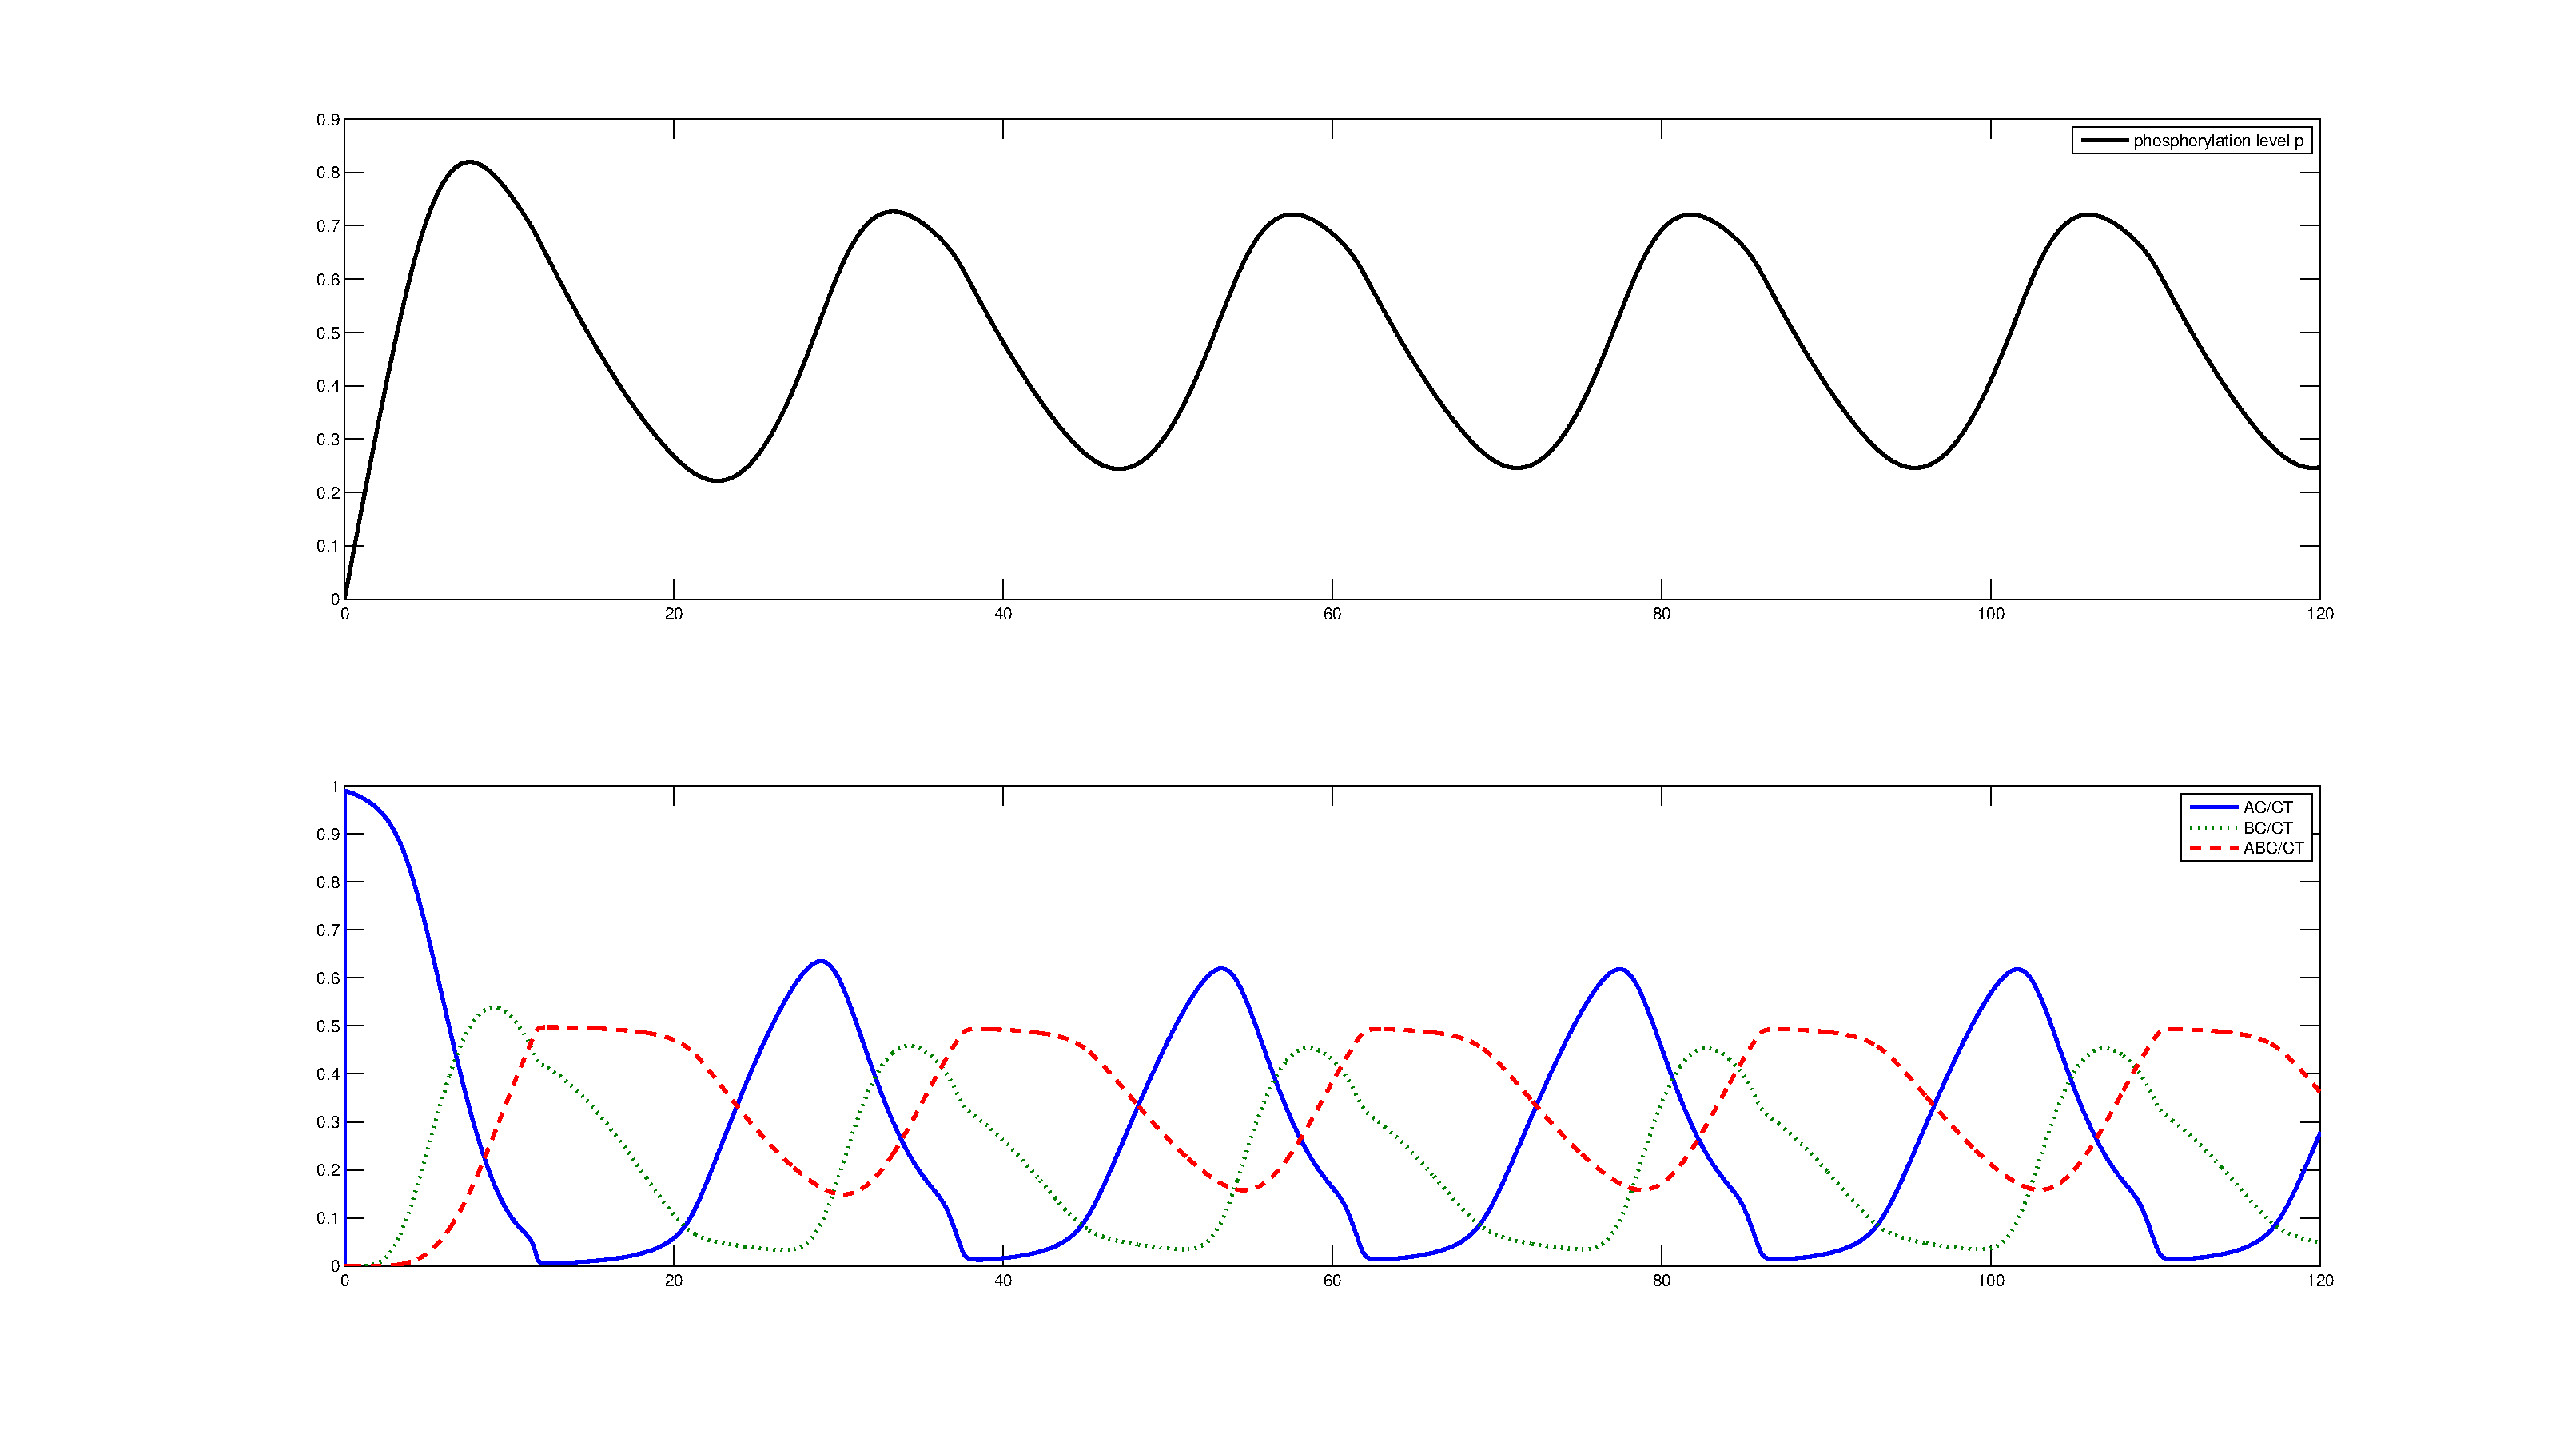
\includegraphics[scale=0.33]{kaiabc.eps}
% \caption{\fontfamily{lmss}\selectfont Simulation results reproduced from the model in \citet{van2007} with same parameters and initial conditions. Top panel is the average phosphoryolation level which can sustain a circadian rhythm. Bottom is a temporal file of different KaiC complexes.}\label{fig:van2007}
% \end{figure}

% \begin{figure}[H]
% \centering
% 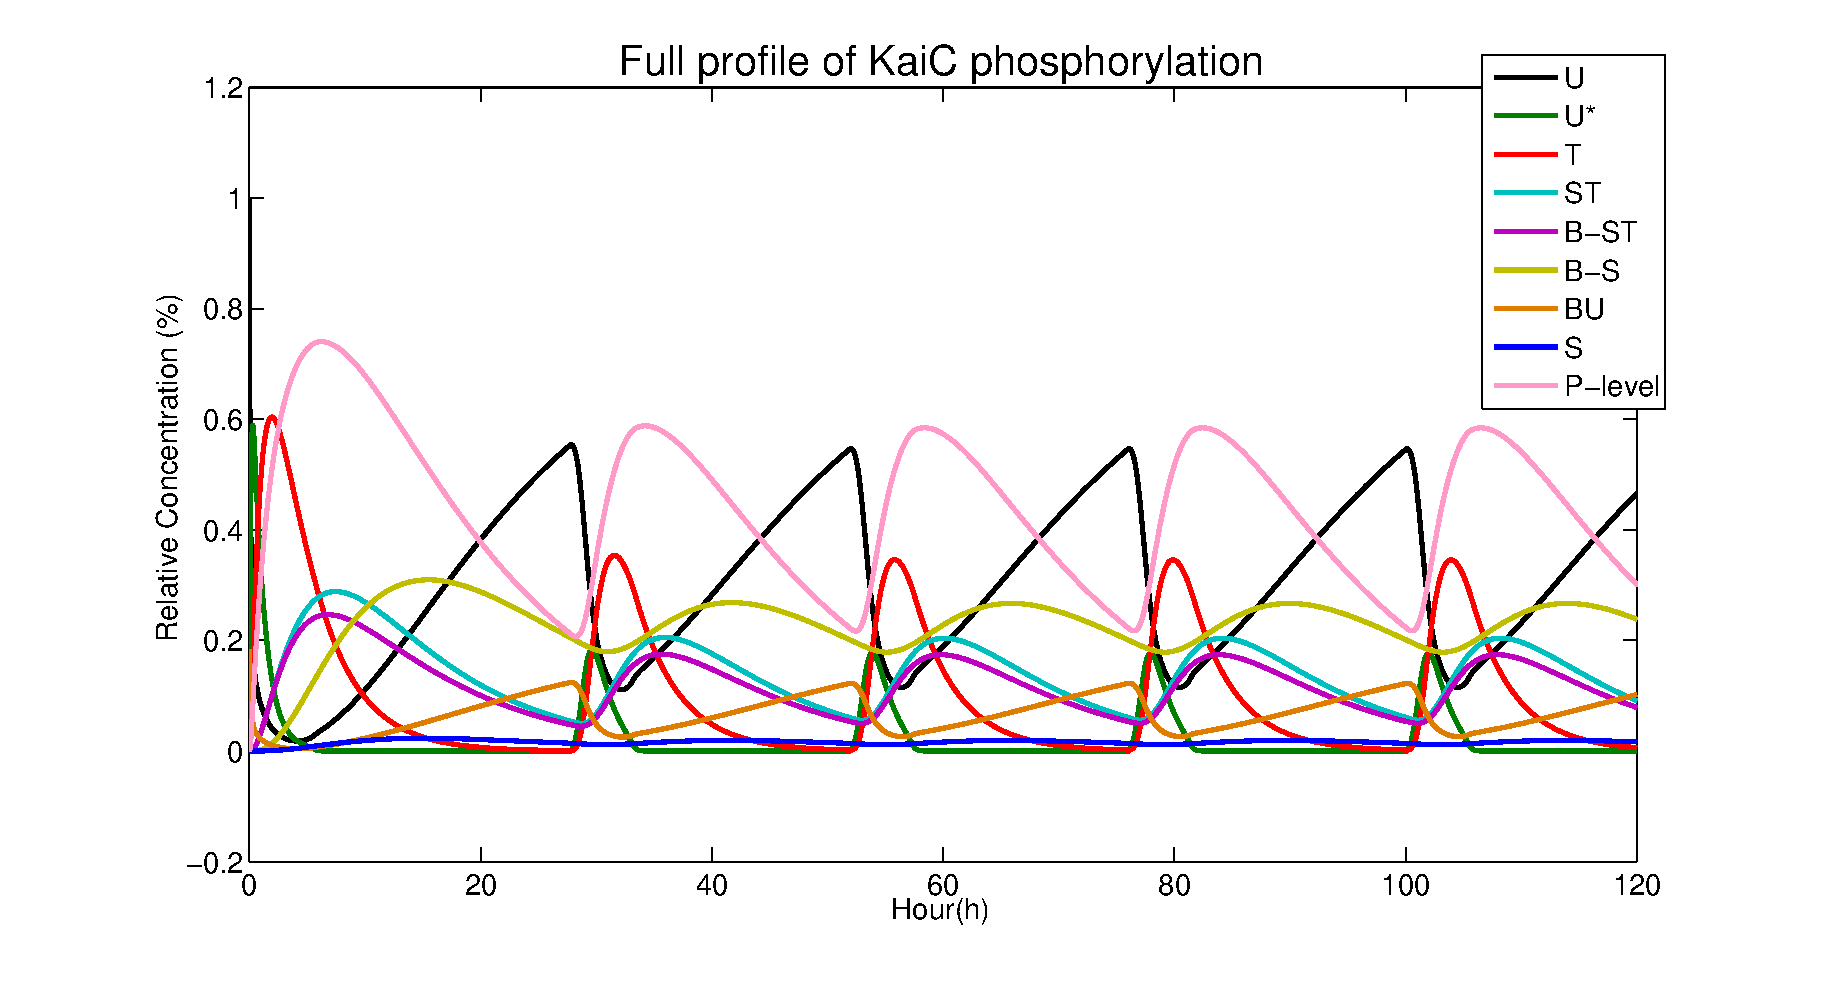
\includegraphics[scale=0.55]{abc24hfull.eps}
% \caption{\fontfamily{lmss}\selectfont Temporal profiles of different KaiC complexes as well as the overall phosphorylation level in the complete KaiABC system. }
% \end{figure}


%Now we simulate the model under the same parameter set as in Fig.\ref{fig:model24_18127} to reproduce some known experimental results. 




%  \begin{figure}[H]
% \centering
% \includegraphics[scale=0.45]{davidtwopar.ps}
% \caption{\fontfamily{lmss}\selectfont Two-parameter bifurcation diagram reproduced from under the same conditions of \citet{van2007}. When $[A]_T/[C]_T$ and $[B]_T/[C]_T$ are given by points inside the region bounded by the blue curve, the system shows stable oscillations. Note that some points on the red curve can not be shown by numerical continuation but we expect the curve to be closed. When  $[A]_T/[C]_T$ and $[B]_T/[C]_T$ are given by points inside the region bounded by the red curve, the system shows bistability.  Parameters taken from all other points give a single steady state.}\label{fig:davidtwopar}
% \end{figure}


\subsection{A Simple Mechanism Revealing Convergent Evolution}
We propose first a simplified model of the cyanobacterial clock where only the KaiA and the KaiC proteins are explicitly included in our system. Although it is well known that the KaiC proteins take the form of hexameric rings both \textit{in vivo} and \textit{in
vitro}, we do not distinguish the KaiC proteins by the number of sub-units phosphorylated in a certain hexamer ring like that in \citet{van2007}. Our goal is to build a relatively simple model that captures the main features in the KaiC system and can produce predictions ready to be tested by experiments. As a result, we start with a model on KaiC monomers (see Fig.\ref{simplemodel}), which can also be considered as a KaiC hexamer model in the sense that all 6 monomer subunits within a hexamer exist in the same phosphorylation states characterized as below.

Two phosphorylation sites, namely Ser-431(S431) and Thr-432(T432), are identified in the work by \citet{nishiwaki2004}. Their results suggest that S431 and T432 phosphorylation sites are indispensable for sustaining circadian rhythm governed by the KaiC phosphorylation cycle. Further experiments and modeling are performed by \citet{rust809}, suggesting that KaiC phosphorylation cycle proceeds in an ordered pattern. Inspired by the results above, we consider KaiC (monomer or hexamer) in four different states: unphosphorylated KaiC ( denoted by U), S431 phosphorylated KaiC (denoted by S), T432 phosphorylated KaiC (denoted by T), S431 \& T432 phosphorylated KaiC (denoted by ST).

We argue that KaiA first facilitates KaiC phosphorylation in a enzymatic way, where the T432 site of KaiC gets phosphorylated before S431 does. This KaiA-enhanced phosphorylation process is much faster than the autophosphorylation. The tight binding between KaiA and the unphosphorylated KaiC ensures that as long as there is a small amount of free KaiA, phosphorylation can proceed rapidly. As the phosphorylation process proceeds, the KaiC proteins become phosphorylated on S432 and start to sequester KaiA proteins through tight binding as indicated in Fig.\ref{simplemodel}. This sequestration scheme is as simplified version which can be extended in our detailed modeling. It can be observed in the simulations of our detailed model that KaiA is indeed mainly sequestered by KaiB through KaiC phosphorylated on S432. (See Fig. \ref{fig:model24_18127})

The system of equations for the system is written in Eq.(\ref{eq:simple}) where the total amount of KaiC protein in the system is denote by $C_T$ and the free amount of KaiA denoted by $[A]$ is computed under equilibrium assumptions similar to \citet{forger2012} (See Supplement Information). 
\begin{equation}\label{eq:simple} 
\begin{aligned}
\frac{d[T]}{dt}&=k_1 [A] (C_T-[T]-[ST]-[S])-k_2 [T]\\
\frac{d[ST]}{dt}&=k_2 [T]-k_3 [ST]\\
\frac{d[S]}{dt}&=k_3 [ST]-k_4 [S]\\
[A]&=\left(A_T-[S]-K_d+\sqrt{(A_T-[S]-K_d)^2+4K_dA_T}\right)/2
\end{aligned}
\end{equation}
Comparing our system with Eq.(\ref{eq:jae_s}) describing the simple mechanism with activator and repressor for the mammalian circadian clock in \citet{forger2012}, we observe similar sequestration mechanism. The activator corresponds to KaiA in our system, while the repressor corresponds to KaiC-S.  

\begin{equation}\label{eq:jae_s} 
\begin{aligned}
\frac{dM}{dt}&=\alpha_1 f(P,A,K_d)-\beta_1 M\\
\frac{dP_c}{dt}&=\alpha_2M-\beta_2 P_c\\
\frac{dP}{dt}&=\alpha_3 P_c-\beta_3 P\\
 f(P,A,K_d)&=\left(A-P-K_d+\sqrt{(A-P-K_d)^2+4K_dA}\right)/2A 
\end{aligned}
\end{equation}

Our simulations and theoretical analysis demonstrates that in this simple model, KaiA sequestration through tight binding with KaiC-S is indispensable for generating oscillations. For different dissociation constant $K_d$ of KaiA sequestration process, we simulate the model with randomly generated parameter sets. For each $K_d$ value of choice, we simulate our model for a total of  $10^5$ randomly generated parameter sets. We plot the fraction of successful simulations against the value of $K_d$ on a log-log plot (Fig. \ref{fig:kd}). Results show that the system is more likely to generate stable oscillations when there is stronger KaiA sequestration (smaller $K_d$), which is consistent with the results in mammalian clock \citet{forger2012}.    




More surprisingly, our results suggest that a stoichiometric balance between the KaiA and KaiC abundance is another key element for generating oscillations. Both theoretical analysis and simulations confirm that a necessary condition for oscillations to occur is \[C_T-(1+r)A_T>\epsilon\] where $r$ is an order 1 constant related to the rates of phosphorylation and dephosphorylation, while $\epsilon$ is a constant of small positive value. Detailed definition of these constants can be found in the Supplement Information. In our simulations, we choose parameter values such that $r=2$ and $\epsilon\ll 1$. The condition then becomes \[C_T-3A_T>\epsilon\] Simulation results verify that parameters that violate this condition can hardly generate oscillations(Fig. \ref{fig:conditioncheck1} and  \ref{fig:conditioncheck2}). A similar mechanism have been proposed in \citet{forger2012} where repressors and activators interacts through tight binding and are in a stoichiometric balance around 1. 




Mathematical analysis also suggests that the simple model in \citet{forger2012} is indeed a limit case of our model as the total amount of (unphosphorylated) KaiC protein goes to infinity, which, we believe, is a condition related to the fact that the additional transcription-translation process in mammalian clock contradicts the conservation law in the cyanobacterial model. 

Despite huge differences between the cyanobacterial and the mammalian clock systems, it is surprising that the core mechanisms of both systems resemble a lot with each other and share similar conditions for generating stable oscillations. Indeed we have demonstrated how convergent evolution happens on a much higher level than it is commonly believed.



\section{Discussion and Future Directions}

Recent experimental studies have proposed a mechanism of dephosphorylation that involves the
ATP Synthase activities \citet{johnson2012,kondo2012}. KaiB monomers are also said to block
ATP binding clefts while forming KaiB$\cdot$KaiC complexes in \citet{villarreal2013}. Therefore, we would like to extend our \textit{in vitro} model by incorporating ATP as well as transcription-translation activities into the system. By studying the extended model, our goal is to explain how energy consumption can remain at a relatively low level in KaiC system.
Comparing our cyanobacterial circadian model with mammalian models such as the one in \citet{forger2012} is also an interesting research direction. 
 \citet{Abe312} has recently proposed that the relative slow rates of phosphorylation is constrained by the slow ATPase activity, which arises from sequestration of a lytic water molecule in an unfavorable position and coupling of ATP hydrolysis to a peptide isomerization with high activation energy. Therefore another difficult research question to ask about the cyanobacterial circadian clock system is whether we can build a structural model that emphasizes more on the structural features over biochemical reactions, which could produce interesting results and predictions. 
 

 
\section{Conclusion}

 Although there are many differences between mammalian and bacterial systems, we have so far discovered a uniform mechanism that enables stable circadian oscillations in both systems. We have shown the connection between the cyanobacterial and mammalian clock by theoretical analysis of the model focusing on mathematical reasoning. We are able to identify and analyzed the core mechanism that drives the oscillations in the KaiC system. This convergent evolution is revealed through the similar sequestration mechanism and the stoichiometric balance between the activator KaiA and inhibitor KaiC. A detailed model is proposed subsequently which can reproduce previous experimental results both qualitatively and quantitatively. 

 \begin{figure}
\centering
\begin{subfigure}{0.7\textwidth}
\centering
\includegraphics[scale=0.52]{core_model.eps}
\caption{}\label{simplemodel}
\end{subfigure}
~
\begin{subfigure}{0.7\textwidth}
\centering
\includegraphics[scale=0.4]{detailed_model.eps}
\caption{}
\label{fig:diagram}
\end{subfigure}
\caption{\fontfamily{lmss} Diagrams for both the simple and the detailed models. (A) The schematic for the simplified cyanobacterial clock model. Squares are proteins in different states, small circles indicates the phosphatase groups on the corresponding sites. Arrows indicate reactions among proteins, the width of which shows the relative strength. (B) Detailed mechanism. Squares are proteins in different states, small circles indicates the phosphatase groups on the corresponding sites. Arrows indicate reactions among proteins, the width of which shows the relative strength.}
\end{figure}

\begin{figure}
\centering
\begin{subfigure}{0.49\textwidth}
\centering
\includegraphics[scale=0.4]{conditioncheck1.eps}
\caption{}\label{fig:conditioncheck1}
\end{subfigure}
~
\begin{subfigure}{0.49\textwidth}
\centering
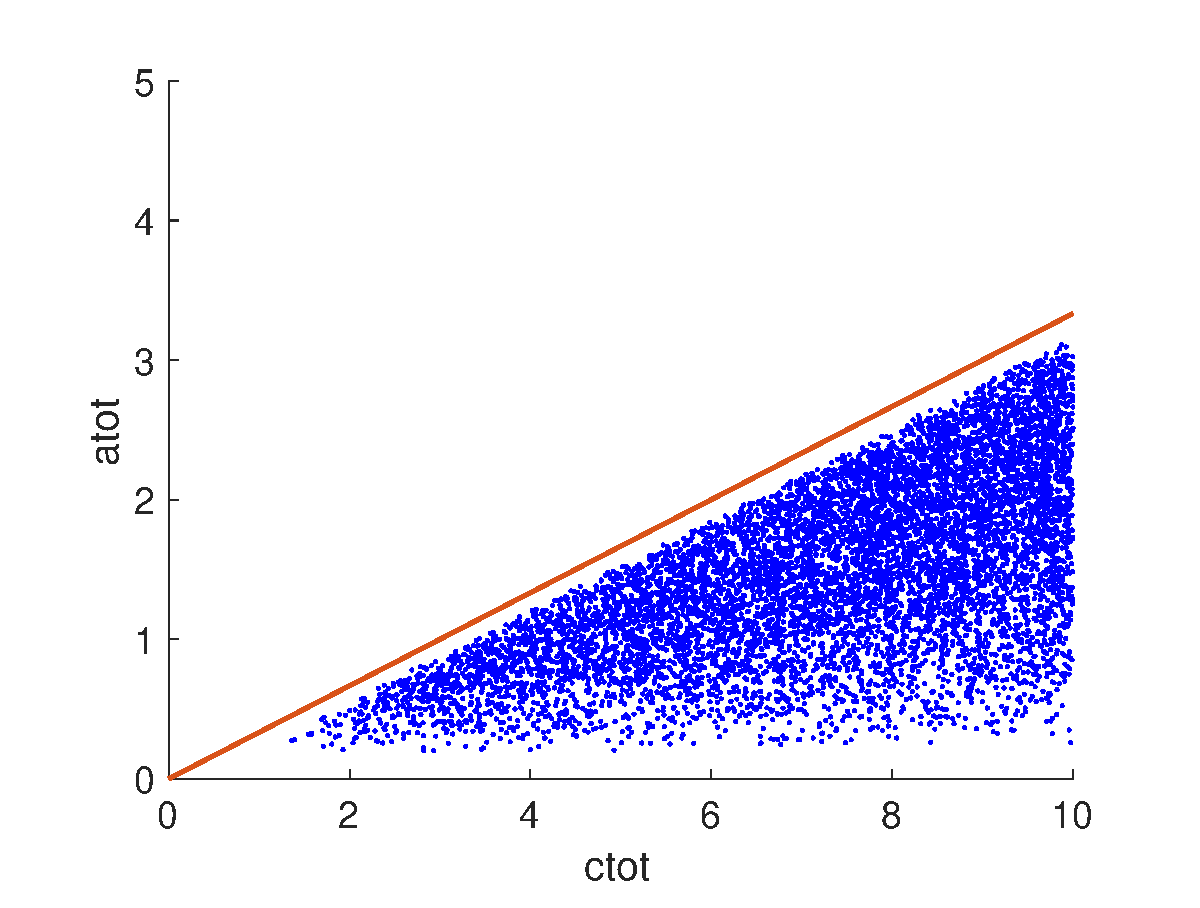
\includegraphics[scale=0.4]{conditioncheck2.eps}
\caption{}\label{fig:conditioncheck2}
\end{subfigure}
~
\begin{subfigure}{0.8\textwidth}
\centering
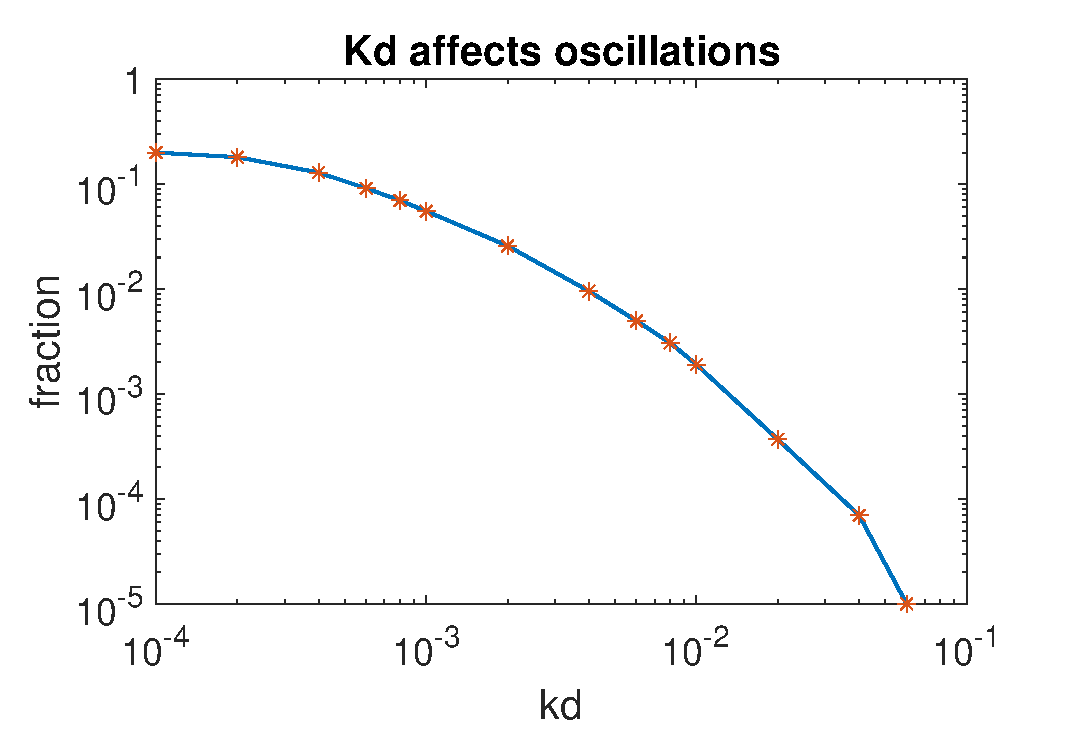
\includegraphics[scale=0.6]{kd.eps}
\caption{}\label{fig:kd}
\end{subfigure}
\caption{\fontfamily{lmss} Simulation results consistent with mathematical analysis. (A) Blue dots are parameter set that allow oscillations while magenta dots are the ones that don't show oscillations. (B) Any parameter set that generates oscillations is located below the line $A_T=\frac{1}{3} C_T$. (C) The model can generate oscillations for a higher fraction of parameter sets as $K_d$ decreases from $10^{-1}$ to $10^{-4}$. The parameter sets are plotted as sample points (indicated by '*') with a fitted curve on a $\log\log$ plot.}
\end{figure}


%\begin{figure}
%\centering
%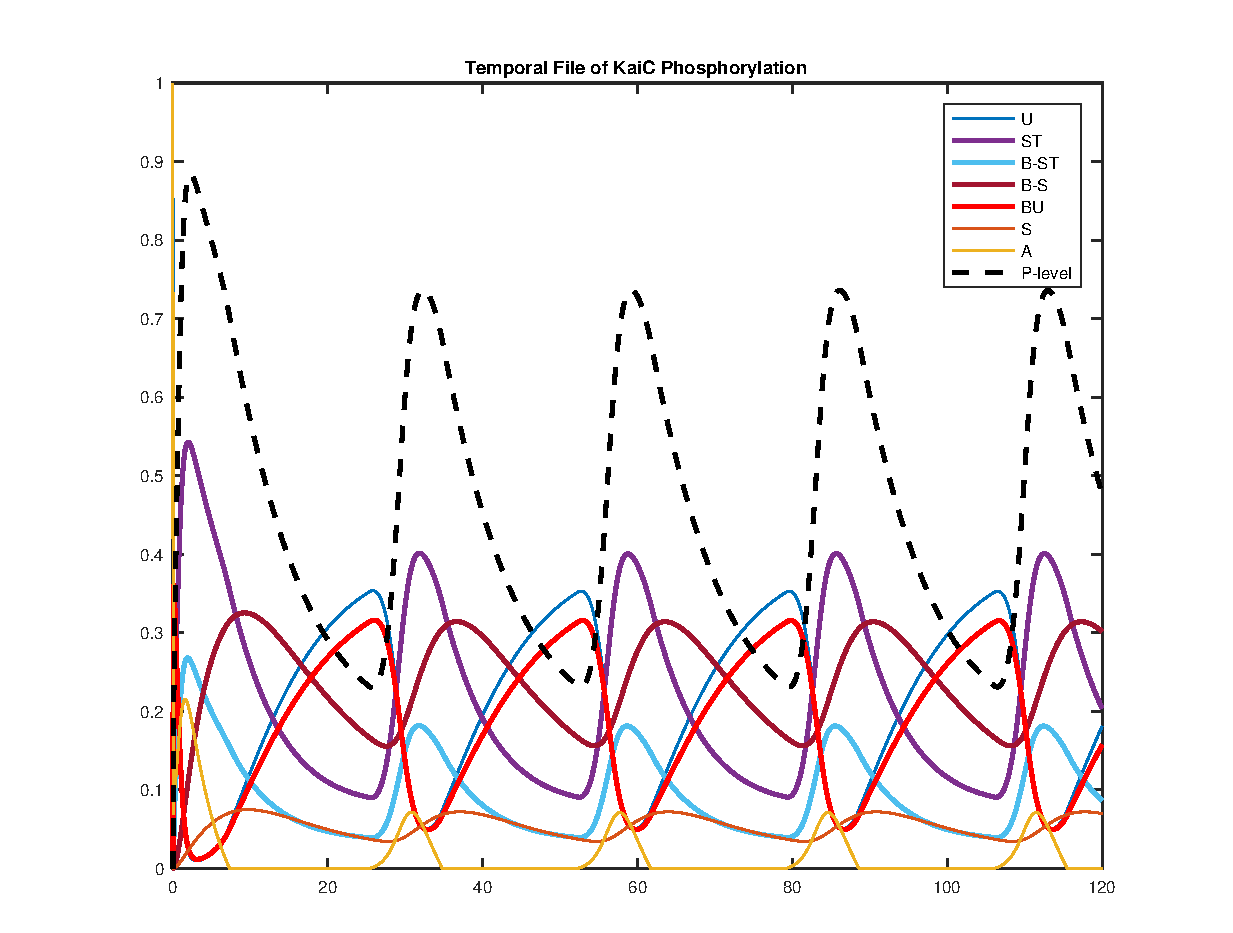
\includegraphics[scale=0.85]{24_18127.eps}
%\caption{\fontfamily{lmss}\selectfont Temporal profiles of different KaiC complexes as well as the overall phosphorylation level in the complete KaiABC system. Notice that KaiBC complexes are combined with the corresponding KaiC, for example, [T] includes both [T] and [B-T]. The proportion of phosphorylated KaiC oscillates between  90\% and 38\% on a circadian period.}
%\label{fig:model24_18127}
%\end{figure}

\begin{figure}
\centering
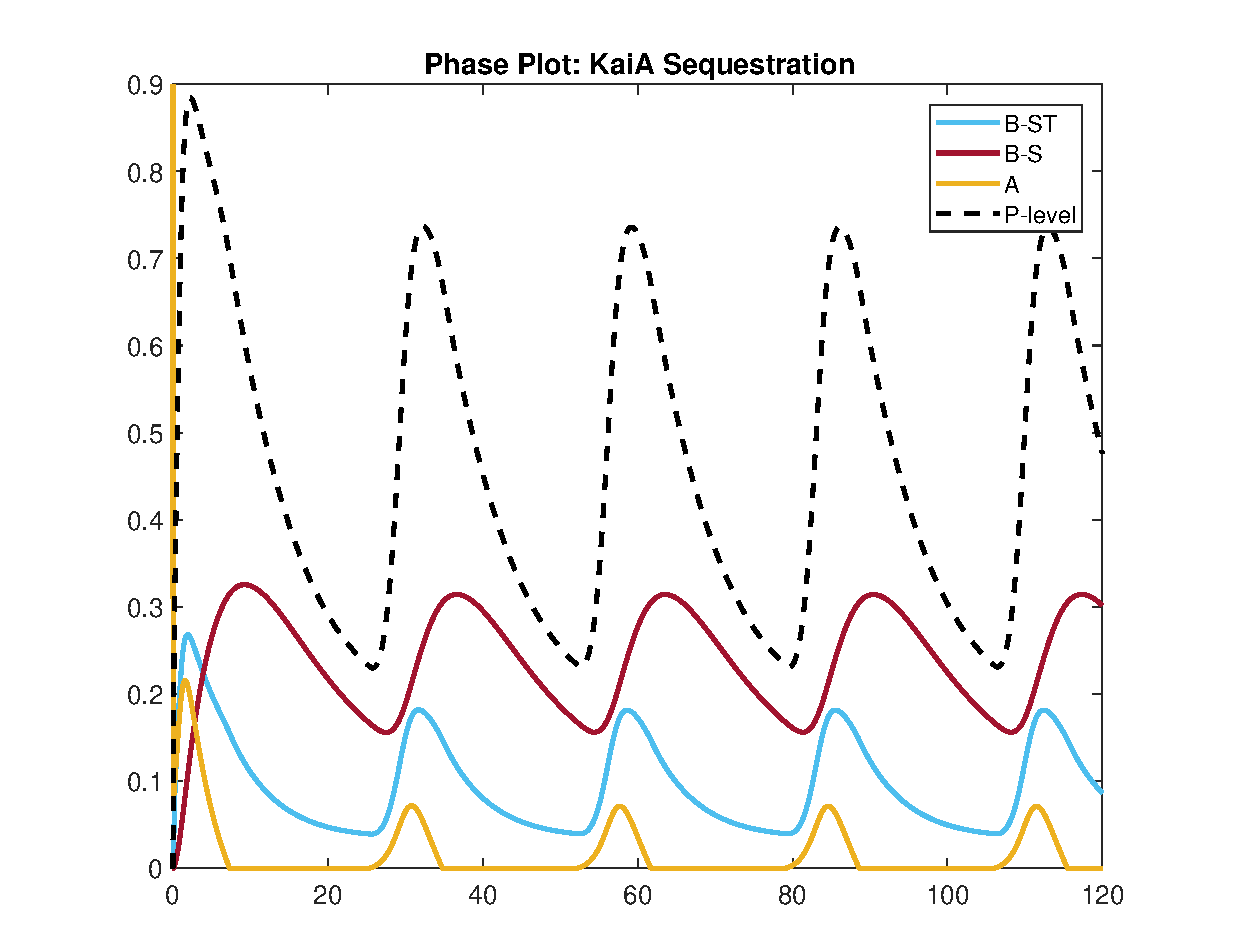
\includegraphics[scale=0.8]{24_18127_Seq_A.eps}
\caption{\fontfamily{lmss}\selectfont Complete phase plot of free KaiA (Yellow), KaiBC complexes (Blue and Magenta) in different stages along with the overall phosphorylation level. The proportion of phosphorylated KaiC (Black) oscillates roughly between  73\% and 25\% on a circadian period. KaiA is mostly sequestered by KaiBC complexes (mainly by B-S) except for a short phase, which correspond to a rapid rise in the phosphorylation level.}
\label{fig:model24_18127}
\end{figure}



%\begin{figure}
%\centering
%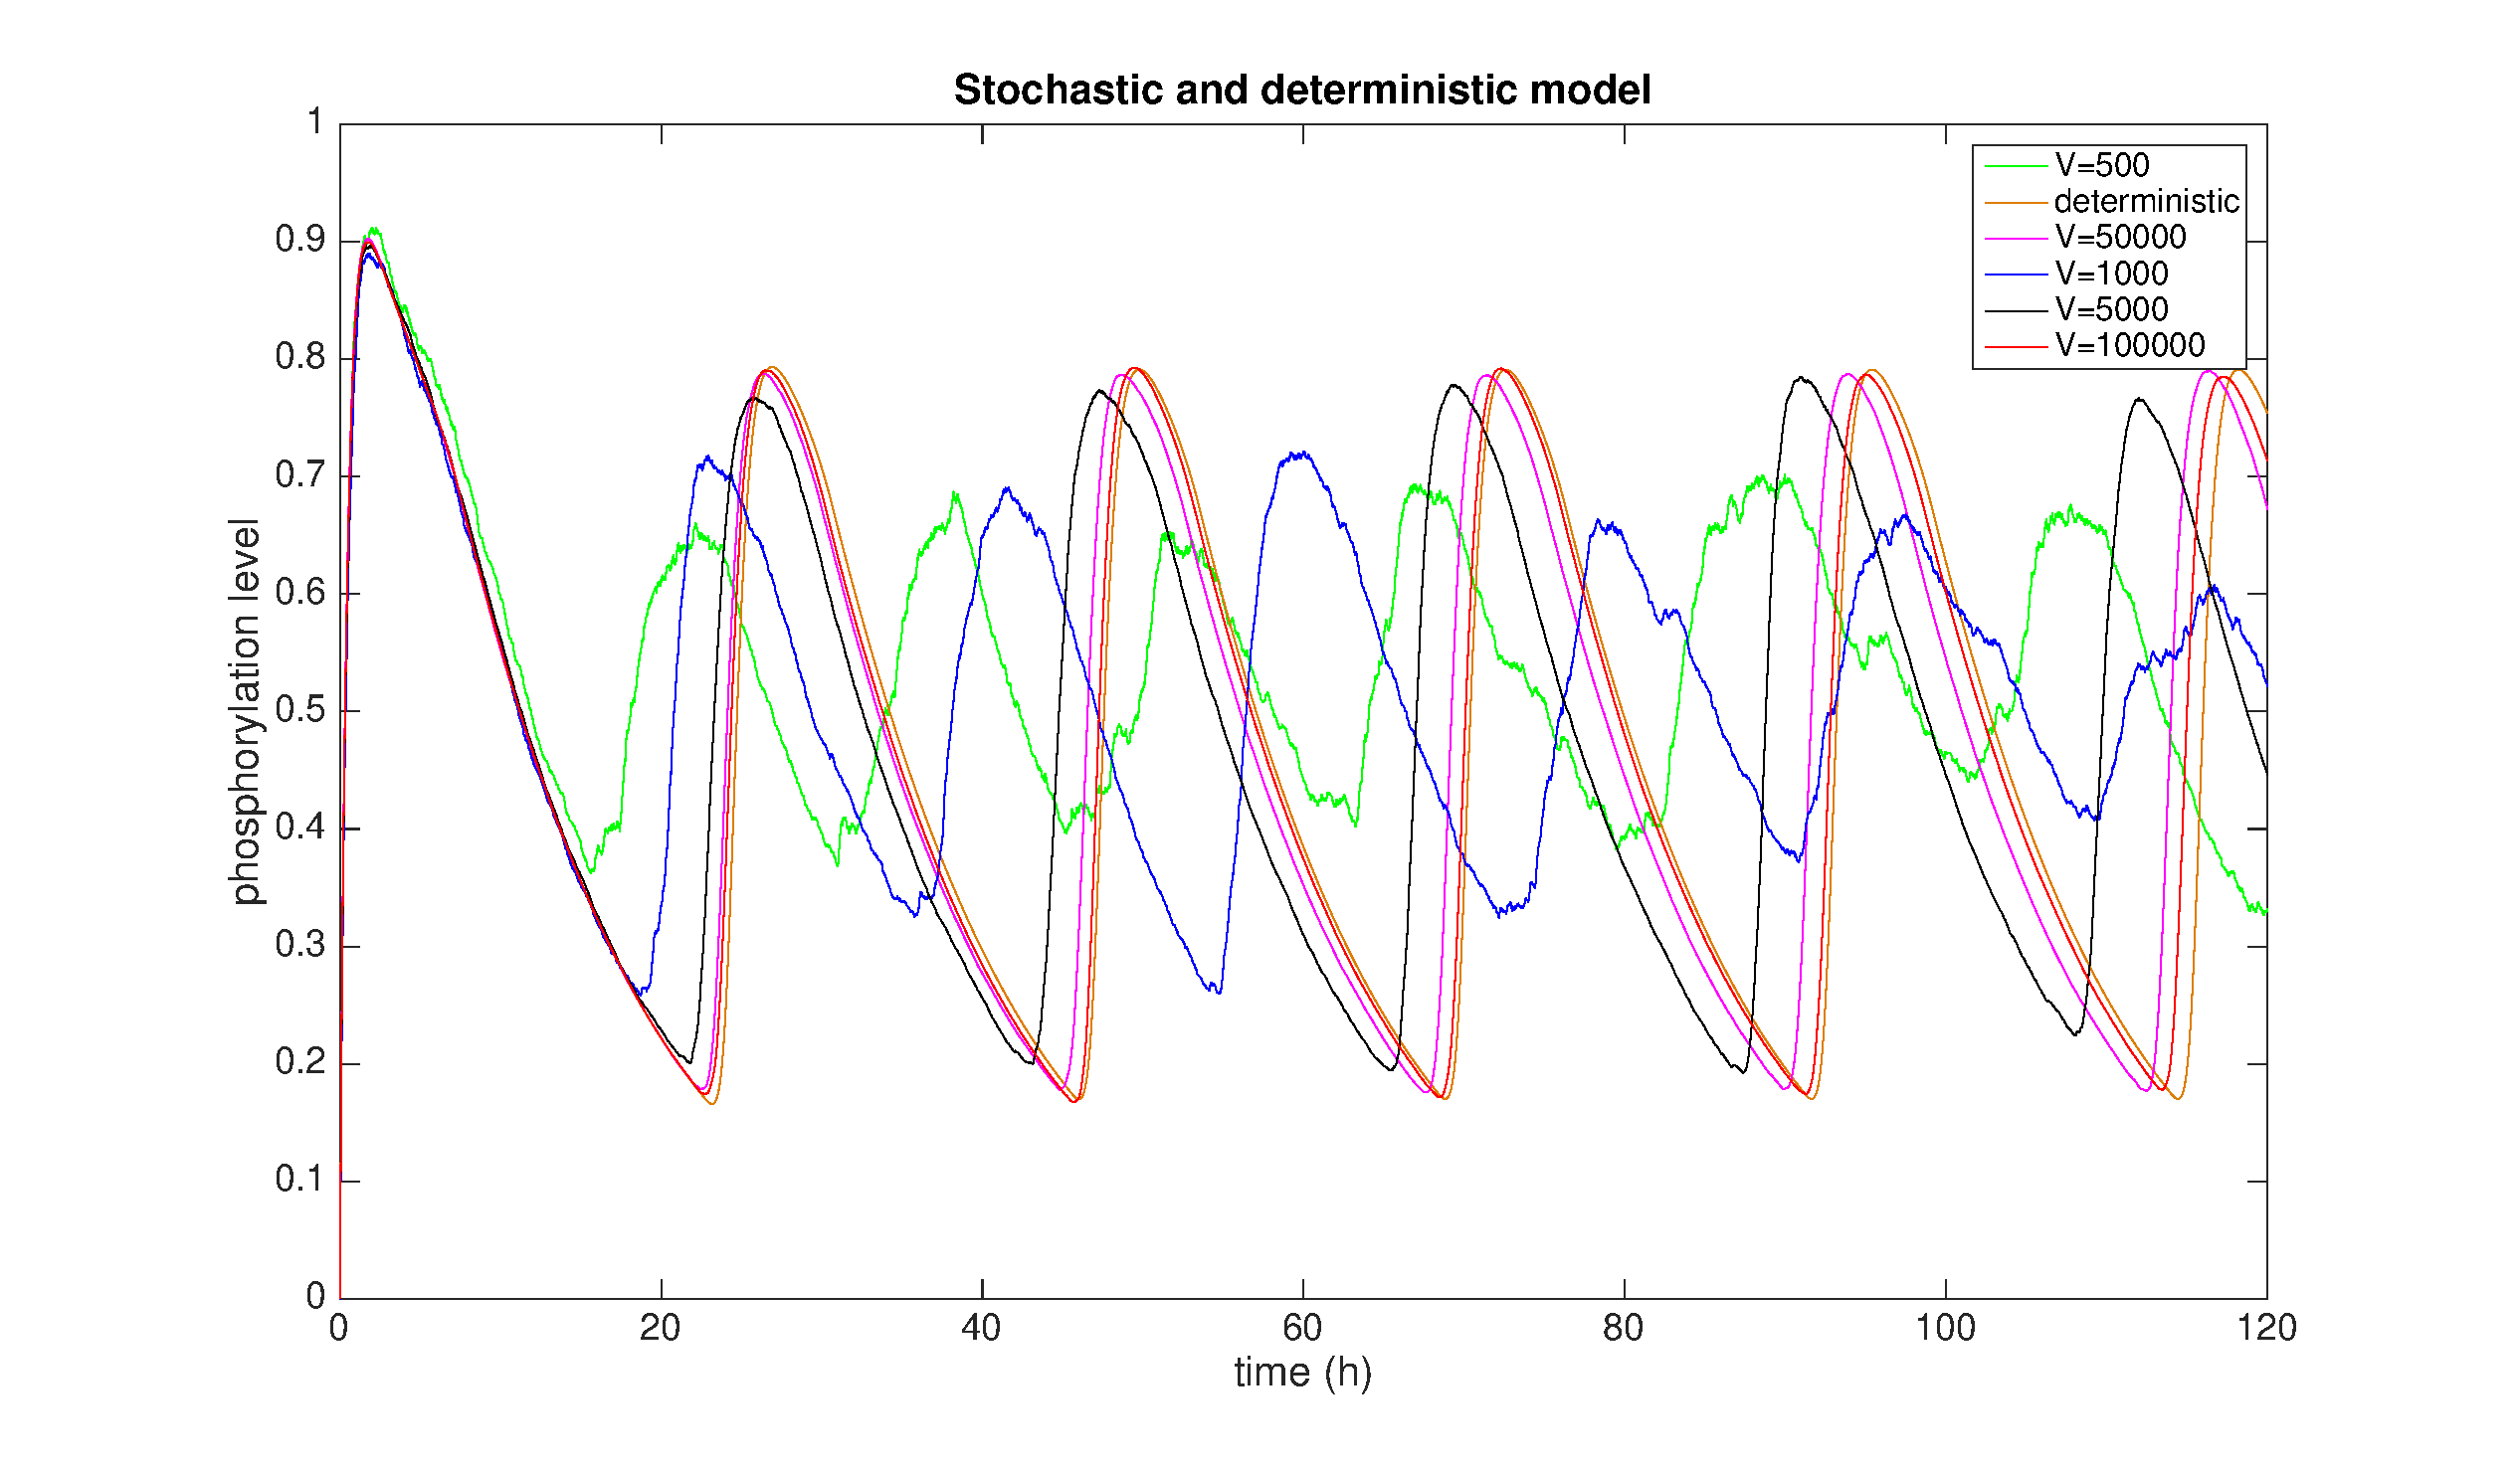
\includegraphics[scale=0.35]{stochastic_deterministic_3_7.eps}
%\caption{\fontfamily{lmss}\selectfont Trajectories from stochastic simulations for various total number of KaiC molecules are compared with that from the continuous model. $V=500,1000,5000,50000,100000$}\label{fig:conVSdisc}
%\end{figure}

\begin{figure}
\centering
\includegraphics[scale=0.18]{comparison.eps}
\caption{\fontfamily{lmss}\selectfont (A-B) Comparison with experimental data from \citet{rust809}. In both results, $\tau_1\approx 9.5$ is the phosphorylation phase time length and $\tau_2\approx18.5$ is the dephosphorylation phase duration. (C-F) Comparison with circadian data from \citet{phong2012},  our model shows a robust period around $24$h under different ATP/ADP ratios. (G-F) Comparison with \citet{phong2012} where we confirmed the importance of CI domain in producing circadian rhythm }\label{fig:comparison}
\end{figure}



\vfill

\section{Supplement Information}
\subsection{Mathematical Model}


In light of much of the experimental results suggesting the importance of KaiB protein in the system, our simple model Eq.\ref{eq:simple} can then be extended to Eq.\ref{eq:full} following the same design rules. We argue that different alternations on the original simple model in does not affect the validity of important results including temperature compensation, which is discussed in detail in a later section.
\begin{equation}
\begin{gathered}
\mathrm U \overset{k_{\mathrm{a}}}{\underset{+\mathrm {KaiA}}{\longrightarrow}} \mathrm U^{*}, \quad \mathrm U \overset{k_{\mathrm {b}}}{\longleftarrow} \mathrm U^{*} \overset{ k_\mathrm {cat}}{\longrightarrow} \mathrm T 
\\ 
\mathrm T \overset{k_{\mathrm{a}}}{\underset{+\mathrm {KaiA}}{\longrightarrow}} \mathrm T^{*},\quad \mathrm T \overset{k_{\mathrm {b}}}{\longleftarrow} \mathrm T^{*} \overset{ k_\mathrm{cat}}{\longrightarrow} \mathrm{ST} \\
\mathrm{U} \overset{ k_\mathrm{ps}}{\longrightarrow} \mathrm{T} \overset{ k_\mathrm{ps}}{\longrightarrow} \mathrm{ST} \\
\mathrm {ST}+\mathrm B\overset{ k_{2}^{\mathrm{on}}}{\underset{k_{2}^{\mathrm{off}}}{\rightleftarrows}} \mathrm {B\cdot ST},\quad \mathrm S+\mathrm B\overset{ k_{3}^{\mathrm{on}}}{\underset{k_{3}^{\mathrm{off}}}{\rightleftarrows}} \mathrm {B\cdot S},\quad \mathrm U+\mathrm B\overset{ k_{1}^{\mathrm{on}}}{\underset{k_{1}^{\mathrm{off}}}{\rightleftarrows}} \mathrm {B\cdot U}\\
\mathrm {B\cdot ST} \overset{ k_{\mathrm{dps}}}{\longrightarrow} \mathrm{B\cdot S}, \quad
\mathrm {B\cdot S} \overset{ k_{\mathrm{dps}}}{\longrightarrow} \mathrm{B\cdot U}\\
 \mathrm{ST} \overset{ k_\mathrm{dps}}{\longrightarrow} \mathrm{S} \overset{ k_\mathrm{dps}}{\longrightarrow} \mathrm{U} \\
\end{gathered}\label{eq:full}
\end{equation}

First model assumes that there are multiple phosphorylation levels of KaiC with differentiated phosphorylation process in each step. Unphosphorylated KaiC binds with KaiA with high affinity and enters an unstable phosphorylation state (KaiC-P$^{*}$), this catalytic process is quick enough that we can assume equilibrium. Another way to understand is that almost immediately after the phosphorylation step, the enzyme KaiA drops off from KaiC. 
Unstable KaiC-P$^{*}$ can then slowly stabilize by either falling back to be unphosphorylated or proceeding forward into a stable phosphorylated state KaiC-P$_{1}$. Once proceeded into a stable phosphorylation state, KaiC-P$_{1}$ go through a few more slow phosphorylation steps. Finally a highly phosphorylated KaiC protein can bind with KaiB into KaiB$\cdot$KaiC complex which sequester KaiA activity by eliminating the free KaiA in a linear fashion. KaiB$\cdot$KaiC complex can then dephosphorylate while still sequestering KaiA. Here we also argue that unlike the complicated phosphorylation phase, KaiC dephosphorylation can proceed in one step at a slow rate. Finally, KaiB falls off the unphosphorylated KaiB$\cdot$KaiC complex, thus freeing more KaiA protein to catalyze the first phosphorylation step and start over another oscillation cycle. 

% The key reactions in this first model are listed below where we denote by U the unphosphorylated KaiC, P$^{*}$ the unstable phosphorylated state and P$_{i}$'s ($i=1,2,3,4$) the stable phosphorylated KaiC states, along with KaiBC complexes represented in a natural way:

% \begin{gather*}
% \mathrm U \overset{k_{\mathrm{a}}}{\underset{+\mathrm {KaiA}}{\longrightarrow}} \mathrm P^{*}\\
% \mathrm U \overset{k_{\mathrm {b}}}{\longleftarrow} \mathrm P^{*} \overset{ k_\mathrm f}{\longrightarrow} \mathrm P_1 \overset{ k_\mathrm{ps}}{\longrightarrow} \mathrm{P_2} \overset{ k_\mathrm{ps}}{\longrightarrow} \mathrm{P_3} \overset{ k_\mathrm{ps}}{\longrightarrow} \mathrm{P_4}\\
% \mathrm P_4+\mathrm B\overset{ k_{2}^{\mathrm{on}}}{\underset{k_{2}^{\mathrm{off}}}{\rightleftarrows}} \mathrm {P_4\cdot B} \\
% \mathrm {P_4\cdot B} \overset{ k_{\mathrm{dps}}}{\longrightarrow} \mathrm{U\cdot B} \\
% \mathrm U+\mathrm B\overset{ k_{1}^{\mathrm{on}}}{\underset{k_{1}^{\mathrm{off}}}{\rightleftarrows}} \mathrm {U\cdot B}
% \end{gather*}
                                                                                               
The corresponding mass action equations are as follows:
\begin{align*}
\frac{d[U]}{dt}&=k_{\mathrm b}[P^{*}]-k_{\mathrm{a}} [A][U]+k_{1}^{\mathrm{off}}[UB] -k_{1}^{\mathrm{on}}[U][B] \\
\frac{d[P^{*}]}{dt}&=k_{\mathrm{ps}} [A][U]-(k_{\mathrm f}+k_{\mathrm b})[P^{*}]\\
\frac{d[P_{1}]}{dt}&=k_{\mathrm f}[P^{*}]-k_{\mathrm{ps}}[P_{1}]\\
\frac{d[P_{i}]}{dt}&=k_{\mathrm{ps}}([P_{i-1}]-[P_{i}]) \quad \mathrm{for} \quad i=2,3\\
\frac{d[P_{4}]}{dt}&=k_{\mathrm{ps}}[P_{3}]+k_{2}^{\mathrm{off}}[BP_{4}] -k_{2}^{\mathrm{on}}[P_{4}][B] \\
\frac{d[P_{4}B]}{dt}&=-k_{\mathrm{dps}}[P_{4}B]-k_{2}^{\mathrm{off}}[P_{4}B] +k_{2}^{\mathrm{on}}[P_{4}][B]\\
\frac{d[UB]}{dt}&=k_{\mathrm{dps}}[P_{4}B]-k_{1}^{\mathrm{off}}[UB] +k_{1}^{\mathrm{on}}[U][B]
\end{align*}

%We also assume that complex P$_{4}$B and UB can both sequester KaiA through tight binding and KaiA unbinds only when KaiB falls off the complex. 

%The sequestration of KaiA is modeled in the following way such that the amount of free KaiA negatively depend on KaiBC complex concentration [UB] and [P$_{4}$B]. Here we choose the strength of binding sequestration of both complexes to be 2, but the choice of strength factor doesn't change the nature of our model. One can also verify that the sequestration scheme is quite robust in the sense that whether [UB] sequesters KaiA or not doesn't affect the qualitative feature. More detailed discussion of whether all the KaiBC complex need to sequester KaiA and whether the choice of sequestration strength affects the oscillation will be in a later section.
\begin{align*}
[B]&=[B]_{T}-[UB]-[P_{4}B]\\
[A]&=\max\{0,[A]_{T}-n\cdot \left([UB]+[P_{4}B]\right) \}\quad n=2
\end{align*}

%Simulating the model we can obtain good oscillations for a wide range of reaction rates parameters. 



\subsection{Linear Stability Analysis}
Here we present mathematical analysis of the simplified model including a linear stability analysis and a limiting procedure. 
We continue to use $[T], [ST], [S]$ as the state variables for KaiC concentrations and $[A]$ the concentration of KaiA. Constants $C_T$ and $A_T$ indicate the total amount of the KaiC and KaiA proteins respectively and $K_d$ is the dissociation constant in the sequestration of KaiA through KaiC-S. We assume that the sequestration happens on a faster timescale, thus reaching equilibrium quickly. Due to the different time scale and the fact that the binding of KaiA doesn't impact other reactions of $S$, we can solve for the concentration of free KaiA.

\begin{gather*}
[A][S_{\mathrm{free}}]=K_d[AS]\\
\implies (A_T-[AS])([S]-[AS])=K_d[AS]\\
\implies 
[AS]=\left(A_T+[S]+K_d-\sqrt{(A_T+[S]+K_d)^2-4A_T[S]}\right)/2\\
\implies 
[A]=A_T-[AS]=\left(A_T-[S]-K_d+\sqrt{(A_T-[S]-K_d)^2+4K_dA_T}\right)/2
\end{gather*}


The system of equations describing the mechanism in Fig. \ref{simplemodel} can therefore be written as follows.  Here we reduce the number of variables by applying the conservation law $[U]=C_T-[T]-[ST]-[S]$.  



\begin{align*}
\frac{\mathrm{d}[T]}{\mathrm{d}t}&=k_1 [A] (C_T-\mathrm{[T]}-\mathrm{[ST]}-\mathrm{[S]})-k_2 \mathrm{[T]}\\
\frac{\mathrm{d}[ST]}{\mathrm{d}t}&=k_2 [T]-k_3 [ST]\\
\frac{\mathrm{d}[S]}{\mathrm{d}t}&=k_3 [ST]-k_4 [S]\\
[A]&=\left(A_T-[S]-K_d+\sqrt{(A_T-[S]-K_d)^2+4K_dA_T}\right)/2
\end{align*}
Our simulation shows that $K_d$ has to be small enough for the system to oscillate. Therefore when $K_d\ll A_T$, we can take limit as $K_d\to 0$ in $[A]$ to get an approximated expression $[A]=\max\{ A_T-[S],0 \}$.
The system is then simplified to:
\begin{align}
\frac{\mathrm{d}[T]}{\mathrm{d}t}&=k_1 (A_T-[S]) (C_T-\mathrm{[T]}-\mathrm{[ST]}-\mathrm{[S]})-k_2 \mathrm{[T]}\label{eq:dt}\\
\frac{\mathrm{d}[ST]}{\mathrm{d}t}&=k_2 [T]-k_3 [ST]\label{eq:dst}\\
\frac{\mathrm{d}[S]}{\mathrm{d}t}&=k_3 [ST]-k_4 [S]\label{eq:ds}
\end{align}

Solving the system for the equilibrium solutions, we obtain $[ST]=\frac{k_4}{k_3} [S],[T]=\frac{k_4}{k_2}  [S]$ from Eq.(\ref{eq:dst}) and Eq. (\ref{eq:ds}). With all other variables plugged in, Eq.(\ref{eq:dt}) can be reduced to a quadratic in terms of $[S]$.
\[k_1(A_T-[S])(C_T-(1+\frac{k_4}{k_2}+\frac{k_4}{k_3})[S])-k_4[S]=0\] 
In addition, we assume $k_4\ll k_1$ since KaiA-enhanced phosphorylation is much faster then (auto)phosphorylation. Hence we can drop the last term $k_4[S]$ in the quadratic equation by dividing $k_1$ through all terms and find two steady state solutions:
\begin{gather*}
(A_T-[S])(C_T-(1+\frac{k_4}{k_2}+\frac{k_4}{k_3})[S])-\frac{k_4}{k_1}[S]=0\\
\implies
(A_T-[S])(C_T-(\frac{k_4}{k_2}+\frac{k_4}{k_3})[S])=0\\
\implies [S]^*=A_T, \quad [S]^*=\frac{C_T}{1+r}, \quad \mathrm{where}\quad r=\frac{k_4}{k_2}+\frac{k_4}{k_3}
\end{gather*}


First, we compute the Jacobian at the second equilibrium $[S]^*=A_T$
\begin{equation}\label{eq:jacobian1}
J_1=
\begin{pmatrix}
-k_2 & 0 & -k_1(C_T-(1+r)A_T)\\
k_2 & -k_3 & 0\\
0 & k_3 & -k_4 
\end{pmatrix}
\end{equation}
The corresponding characteristic function is then:
\[f_2(\lambda)=(\lambda+k_2)(\lambda+k_3)(\lambda+k_4)+k_1k_2k_3(C_T-(1+r)A_T)\]
We conclude from the secant condition that oscillations occur when 
\begin{gather*}
\frac{k_1k_2k_3(C_T-(1+r)A_T)}{k_2k_3k_4}\geq (\sec (\frac{\pi}{3}))^3
\end{gather*}
\begin{equation}\label{eq:ctatcondition}
C_T-(1+r)A_T\geq \frac{8k_4}{k_1}
\end{equation}
To verify our analysis, we simulate the model when $k_2=k_3=k_4=0.1$ and compare our results with $C_T-3A_T>\frac{0.8}{k_4}$. 

In order to analyze the Jacobian matrix at the second equilibrium without introducing too much computational details, we further assume that $k_2=k_3=k_4$ which means the autodephosphorylation and the autphosphorylation of KaiC are on the same time scale.
The Jacobian  $[S]^*=\frac{C_T}{3}$  can be then simplified

\begin{equation}\label{eq:jacobian2}
J_2=
\begin{pmatrix}
-k_1(A_T-\frac{C_T}{3})-k_2 & -k_1(A_T-\frac{C_T}{3}) & -k_1(A_T-\frac{C_T}{3})\\
k_2 & -k_2 & 0\\
0 & k_2 & -k_2 
\end{pmatrix}
\end{equation}
The characteristic function of \ref{eq:jacobian2} is a cubic function:
\begin{equation}
\begin{split}
f_2(\lambda)&=(b+k_2+\lambda)(k_2+\lambda)^2+bk_2(k_2+\lambda)+bk_2^2\\
&=(\lambda+k_2)^3+b(k_2+\lambda)^2+bk_2(k_2+\lambda)+bk_2^2\\
&=\lambda^3+(3k_2+b)\lambda^2+(3k_2^2+3bk_2)\lambda+k_2^3+3bk_2^2
\end{split}
\end{equation}
where $b=k_1(A_T-\frac{C_T}{3})>0$.

The Routh-Hurwitz Stability Criterion tells us that a necessary condition for a cubic function $h(x)=x^3+a_2x^2+a_1x+a_0$ to be stable (all of its roots have negative real part) is $a_0>0, a_2>0, a_2a_1>a_0$.

Applying this to our cubic function above, we already have $a_0>0,a_2>0$ and we compute the third one accordingly:
\begin{equation}
\begin{split}
a_1a_2-a_0&=(3k_2+b)(3k_2^2+3bk_2)-k_2^3+3bk_2^2\\&
=(3k_2+b)(3k_2+3b)-k_2^2+3bk_2\\&
=8k_2^2+9bk_2+3b^2\\
&>0 \qquad \qquad \forall\; b,k_2>0
\end{split}
\end{equation}
Therefore we know that all three roots of the characteristic function always have nagative roots, meaning the steady state is stable and there is no oscillations around that point.


\subsection{Stochastic  simulations}
A Markov chain alternative model is also simulated using Gillespie algorithm, a method similar to the kinetic Monte Carlo methods. Trajectories are generated for different values of the  total number of KaiC molecules while keeping the KaiC total concentration a constant $C_T=1 \mu M$. Then the corresponding phophorylation levels of KaiC are plotted (Fig.\ref{fig:Vfrom10to10000}). When the number of molecules is low ($V=10,20,50$), the trajectory does show randomness but there is hardly any sustained oscillations. As the number of KaiC molecules increases, the corresponding oscillations become more stable. When the number of molecules $V$ becomes large enough, the general shape of the profile stays almost the same even if the number is doubled from $V=5000$ to $V=10000$.

To further investigate the relationship between the simulation results from stochastic and deterministic  models, we select a few stochastic trajectories and compare them with the deterministic profile (Fig.\ref{fig:conVSdisc}). The amplitude of the oscillations from stochastic simulation approaches that from the deterministic model as the number of molecules increases. Besides, the phase difference between the stochastic and deterministic simulations decreases significantly as the number of molecules increases. We therefore predicts that in order to observe stable oscillations, the total amount of KaiC proteins in abundance must be above a certain threshold, which we identified to be about $8*10^{-14} \mu \text{mol}$. 

\begin{figure}
\centering
\begin{subfigure}{0.8\textwidth}
\centering
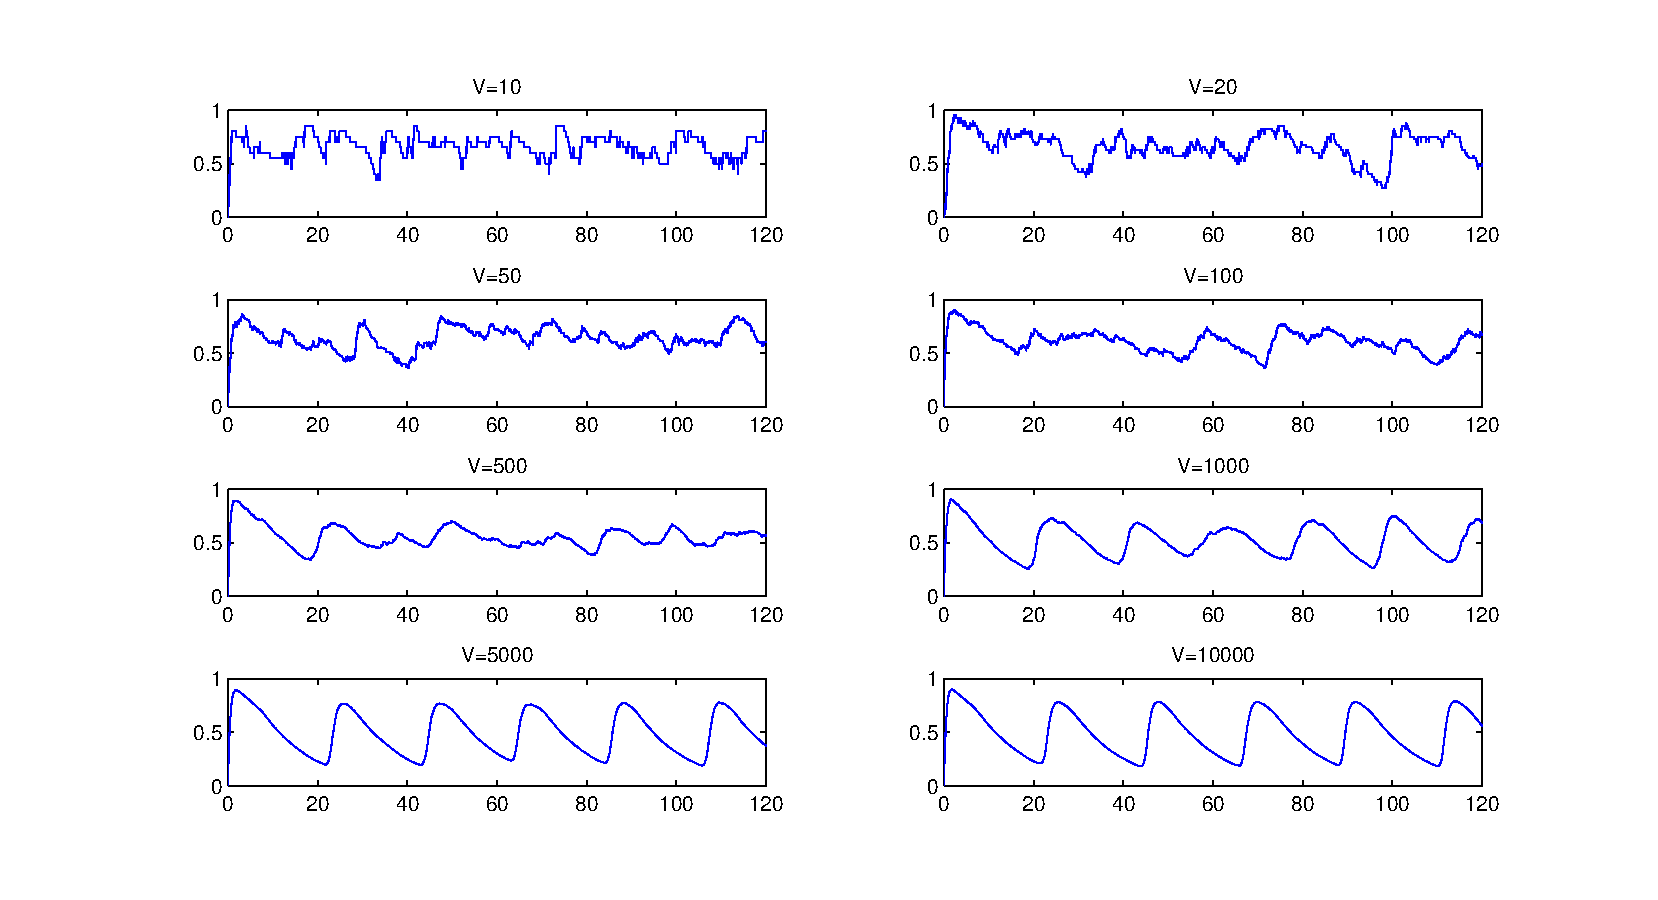
\includegraphics[scale=0.5]{vfrom10to10000.eps}
\caption{}\label{fig:Vfrom10to10000}
\end{subfigure}
\quad
\begin{subfigure}{0.8\textwidth}
\centering
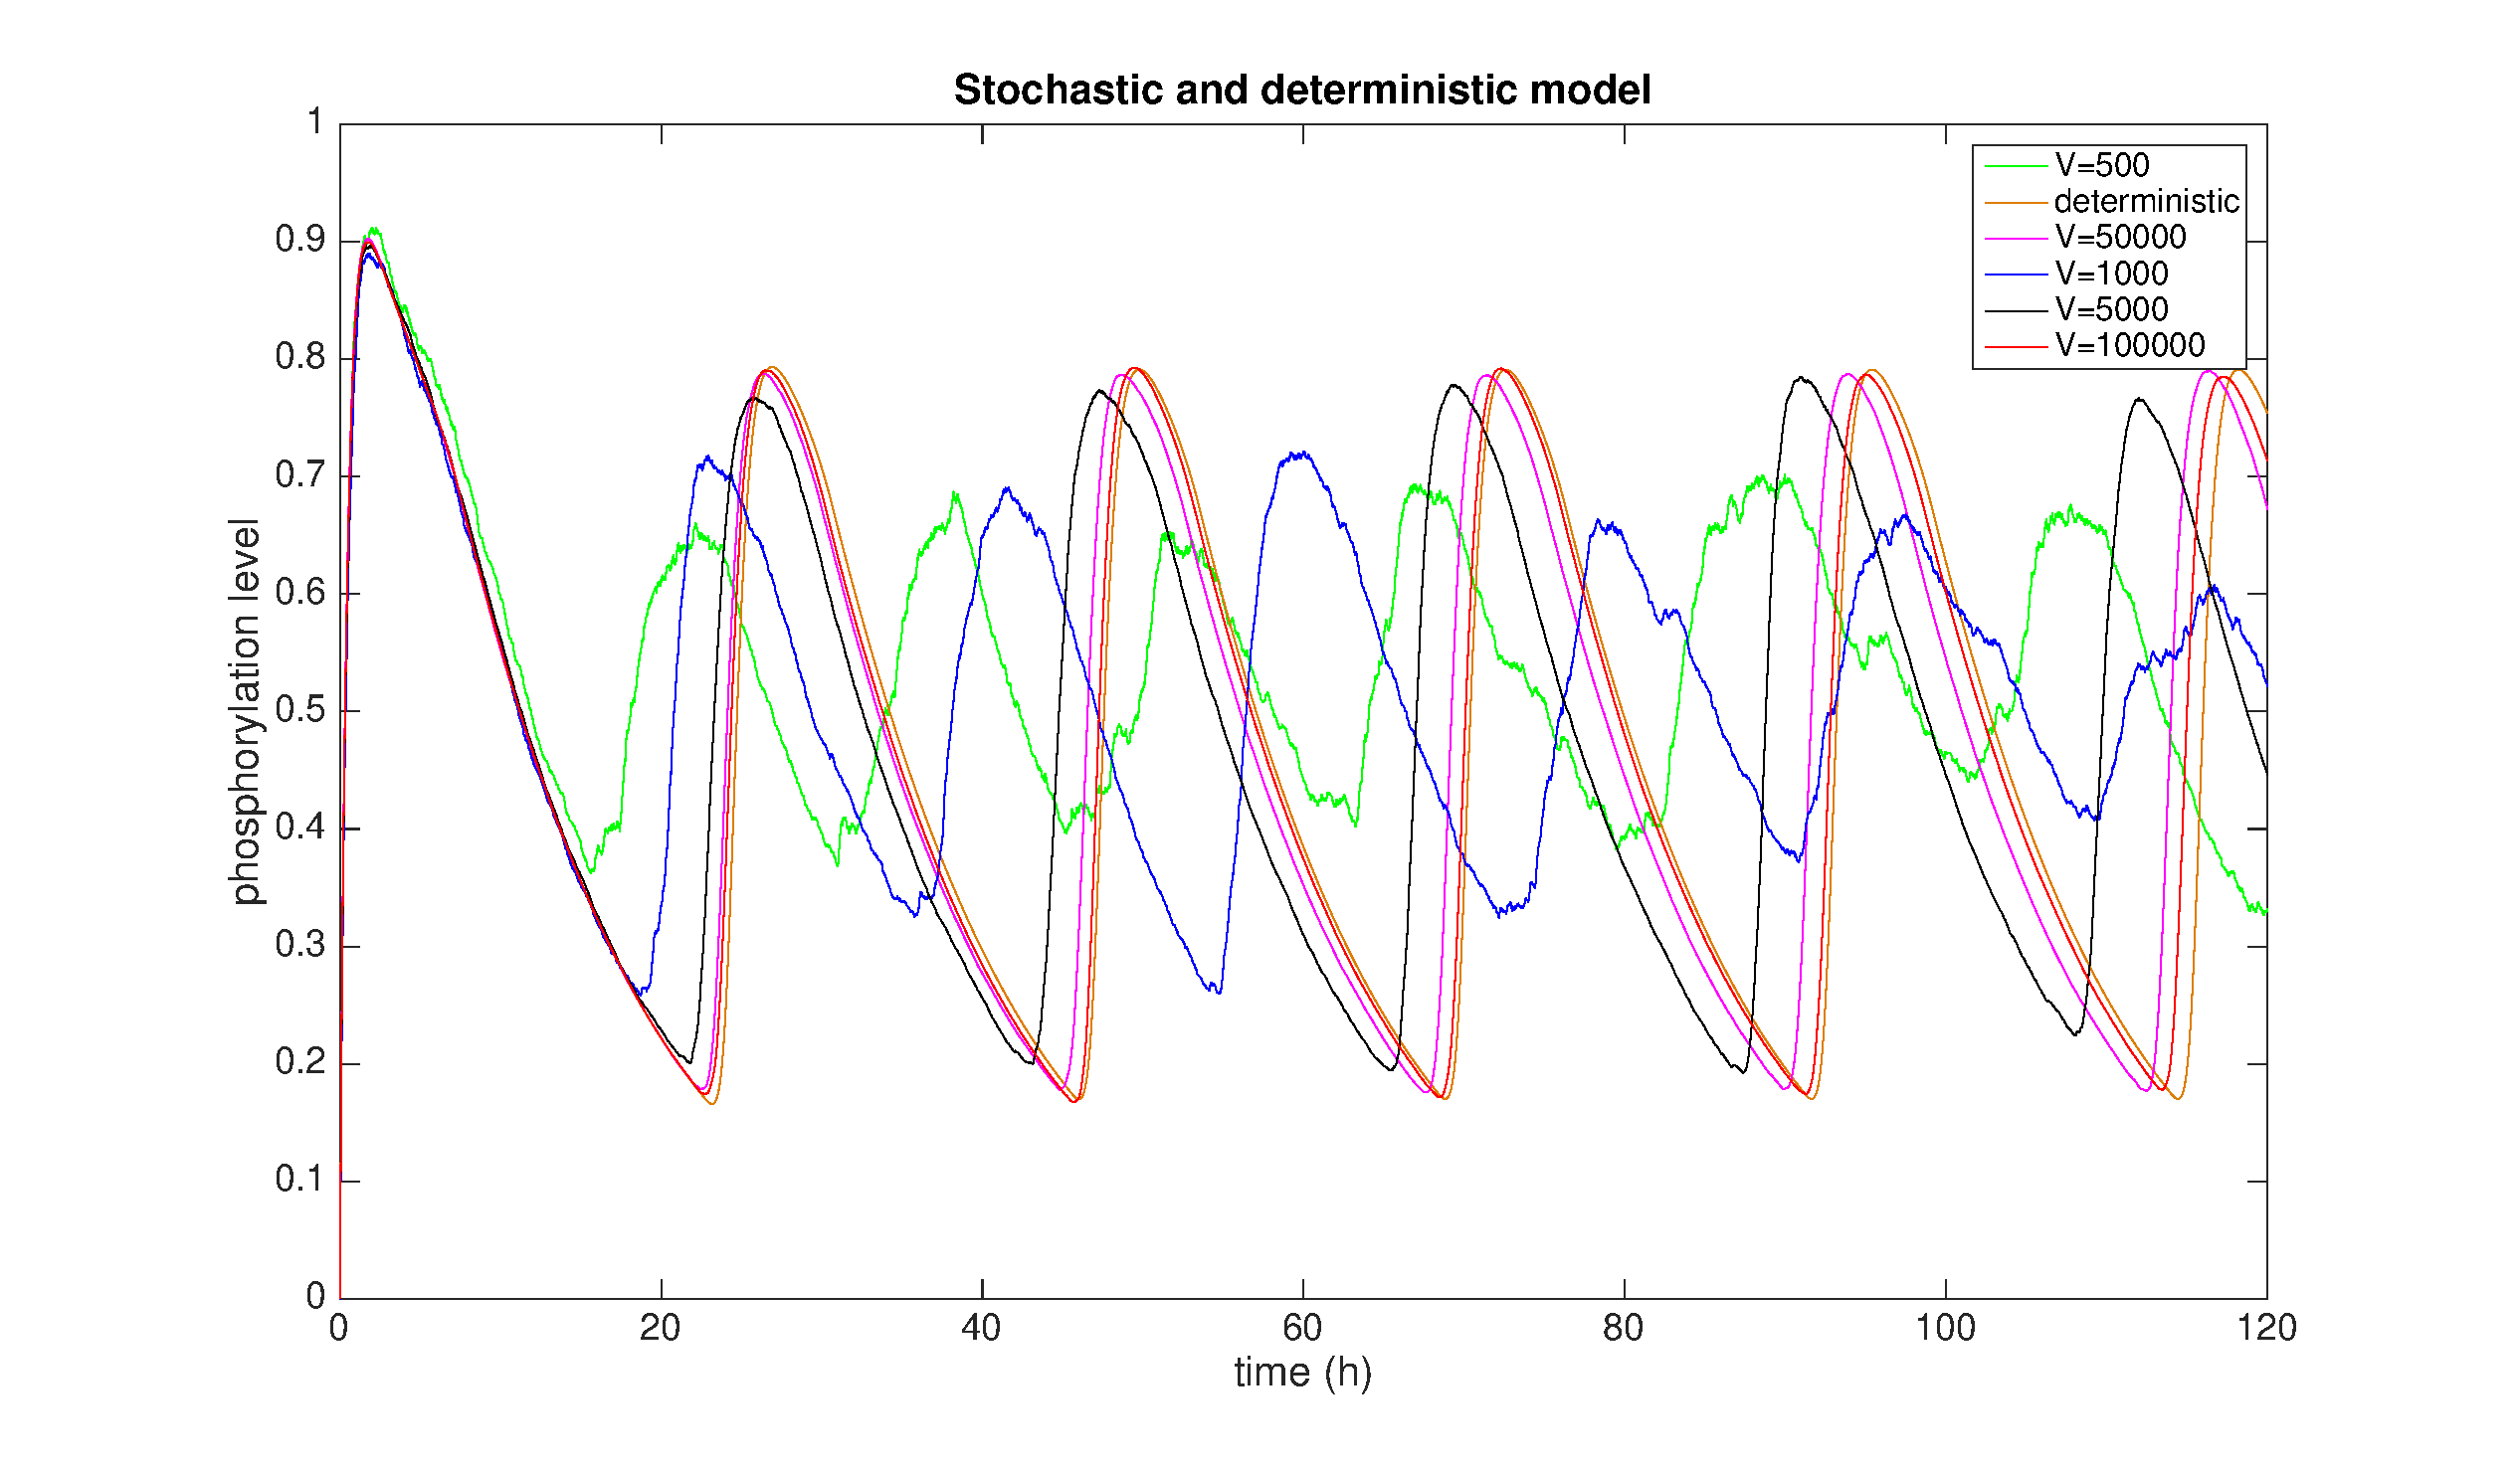
\includegraphics[scale=0.3]{stochastic_deterministic_3_7.eps}
\caption{}\label{fig:conVSdisc}
\end{subfigure}
\caption{\fontfamily{lmss}\selectfont (a)  Trajectories from stochastic simulations for various total number of KaiC molecules  are compared altogether. The horizontal axis of all plots are 'time(h)' while the vertical axis shows the  relative phophorylation level of KaiC protein.  $V=10$,$20$,$50$,$100$,$500$,$1000$,$5000$,$10000$. (b) Trajectories from stochastic simulations for various total number of KaiC molecules are compared with that from the continuous model. $V=500,1000,5000,50000,100000$}
\end{figure}

\subsection{Reproducing experimental results}

Notice that the choice of parameter set does not change any quantitative results. Our model is simulated with different initial conditions to produce dynamics under different situations when it is incubated with KaiA only (Fig\ref{fig:A+C}), KaiB only  (Fig \ref{fig:B+C}) and alone (Fig \ref{fig:conly}). 

Existing experimental results from \citet{kitayama2003} suggest that KaiB alone does not affect the (de)phosphorylation process of KaiC. Indeed we observe from our simulations that the profile of KaiC doesn't change much when KaiB is added into the system. Without KaiA, adding KaiB to KaiC produces the same phosphorylation profile (see Fig.\ref{fig:B+C} and Fig.\ref{fig:conly}).

We have also generated bifurcation diagrams for our model using XPP-AUTO . Our bifurcation diagrams present similar property as that in \citet{van2007}, in that we  also make predictions that oscillations occur when the relative concentration of KaiA (to that of KaiC) is within a certain range while the relative concentration of KaiB doesn't have much effect on whether there are oscillations or not in the system (See Fig. \ref{fig:model18bifur} and \ref{fig:model18twopar}). 
\begin{figure}[H]
\centering
\includegraphics[scale=0.45]{model18bifur.ps}
\caption{\fontfamily{lmss}\selectfont Bifurcation diagram of parameter atoc (fraction of [KaiA] to [KaiC]). Black points represent unstable equilibrium while red points represent stable equilibrium. Branches represent the limit cycle and we observe a supercritical bifurcation within this specific parameter range. }\label{fig:model18bifur}
\end{figure}


\begin{figure}[H]
\centering
\includegraphics[scale=0.45]{model18twopar.ps}
\caption{ \fontfamily{lmss}\selectfont This is a two parameter bifurcation diagram of the KaiC system. atoc is the fraction of KaiA concentration to KaiC concentration. btoc is the fraction of KaiB concentration to KaiC concentration. Points within the region enclosed by the blue curve give initial distributions that can produce oscillations while we expect no oscillations outside this region. }\label{fig:model18twopar}
\end{figure}


\begin{figure}[H]
\centering
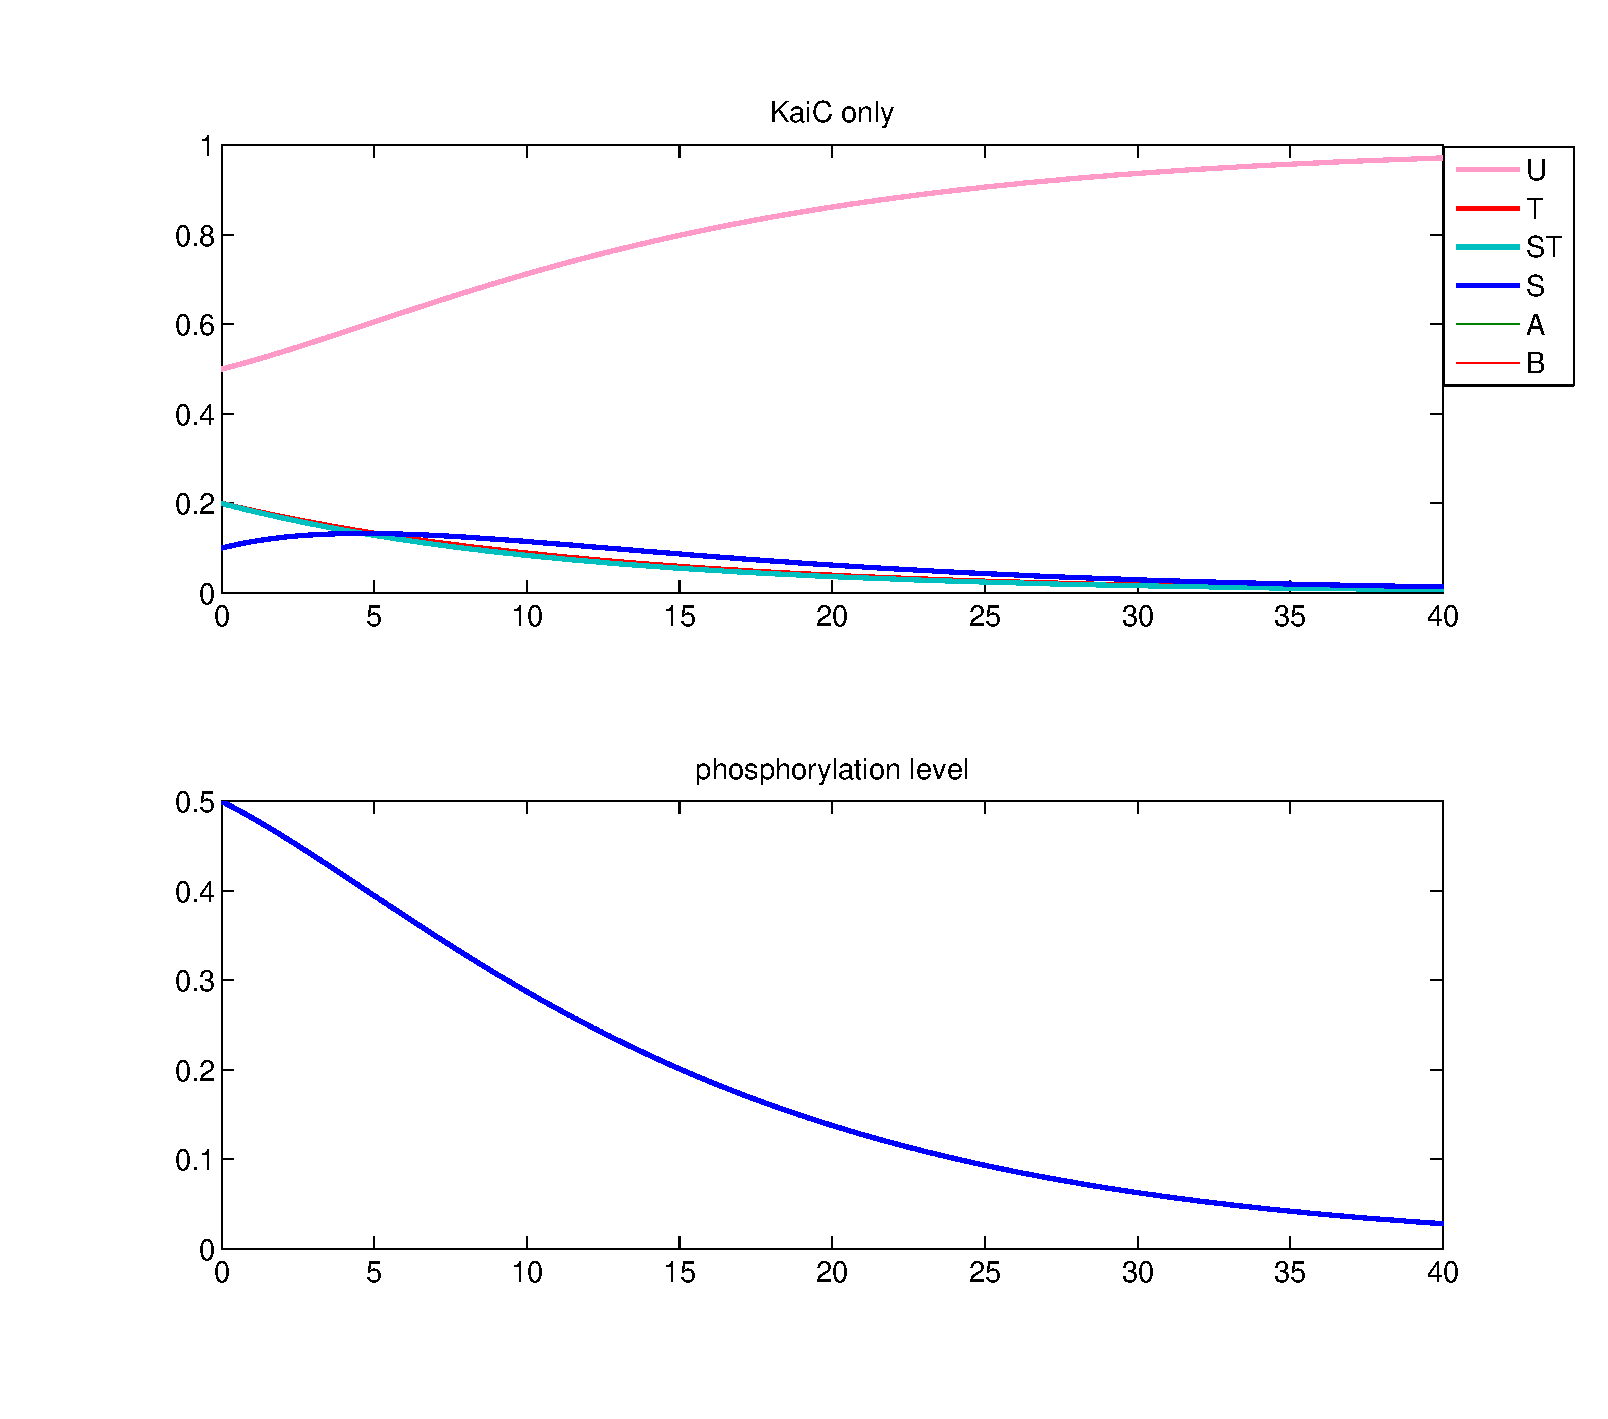
\includegraphics[scale=0.6]{Conly.eps}
\caption{\fontfamily{lmss}\selectfont Temporal profiles of different KaiC complexes as well as the overall phosphorylation level without any KaiA or KaiB in the system. Initially KaiC is 50\% phosphorylated. Complexes that remain zero concentration due to initial conditions are omitted in the graph.}
\label{fig:conly}
\end{figure}

\begin{figure}
\centering
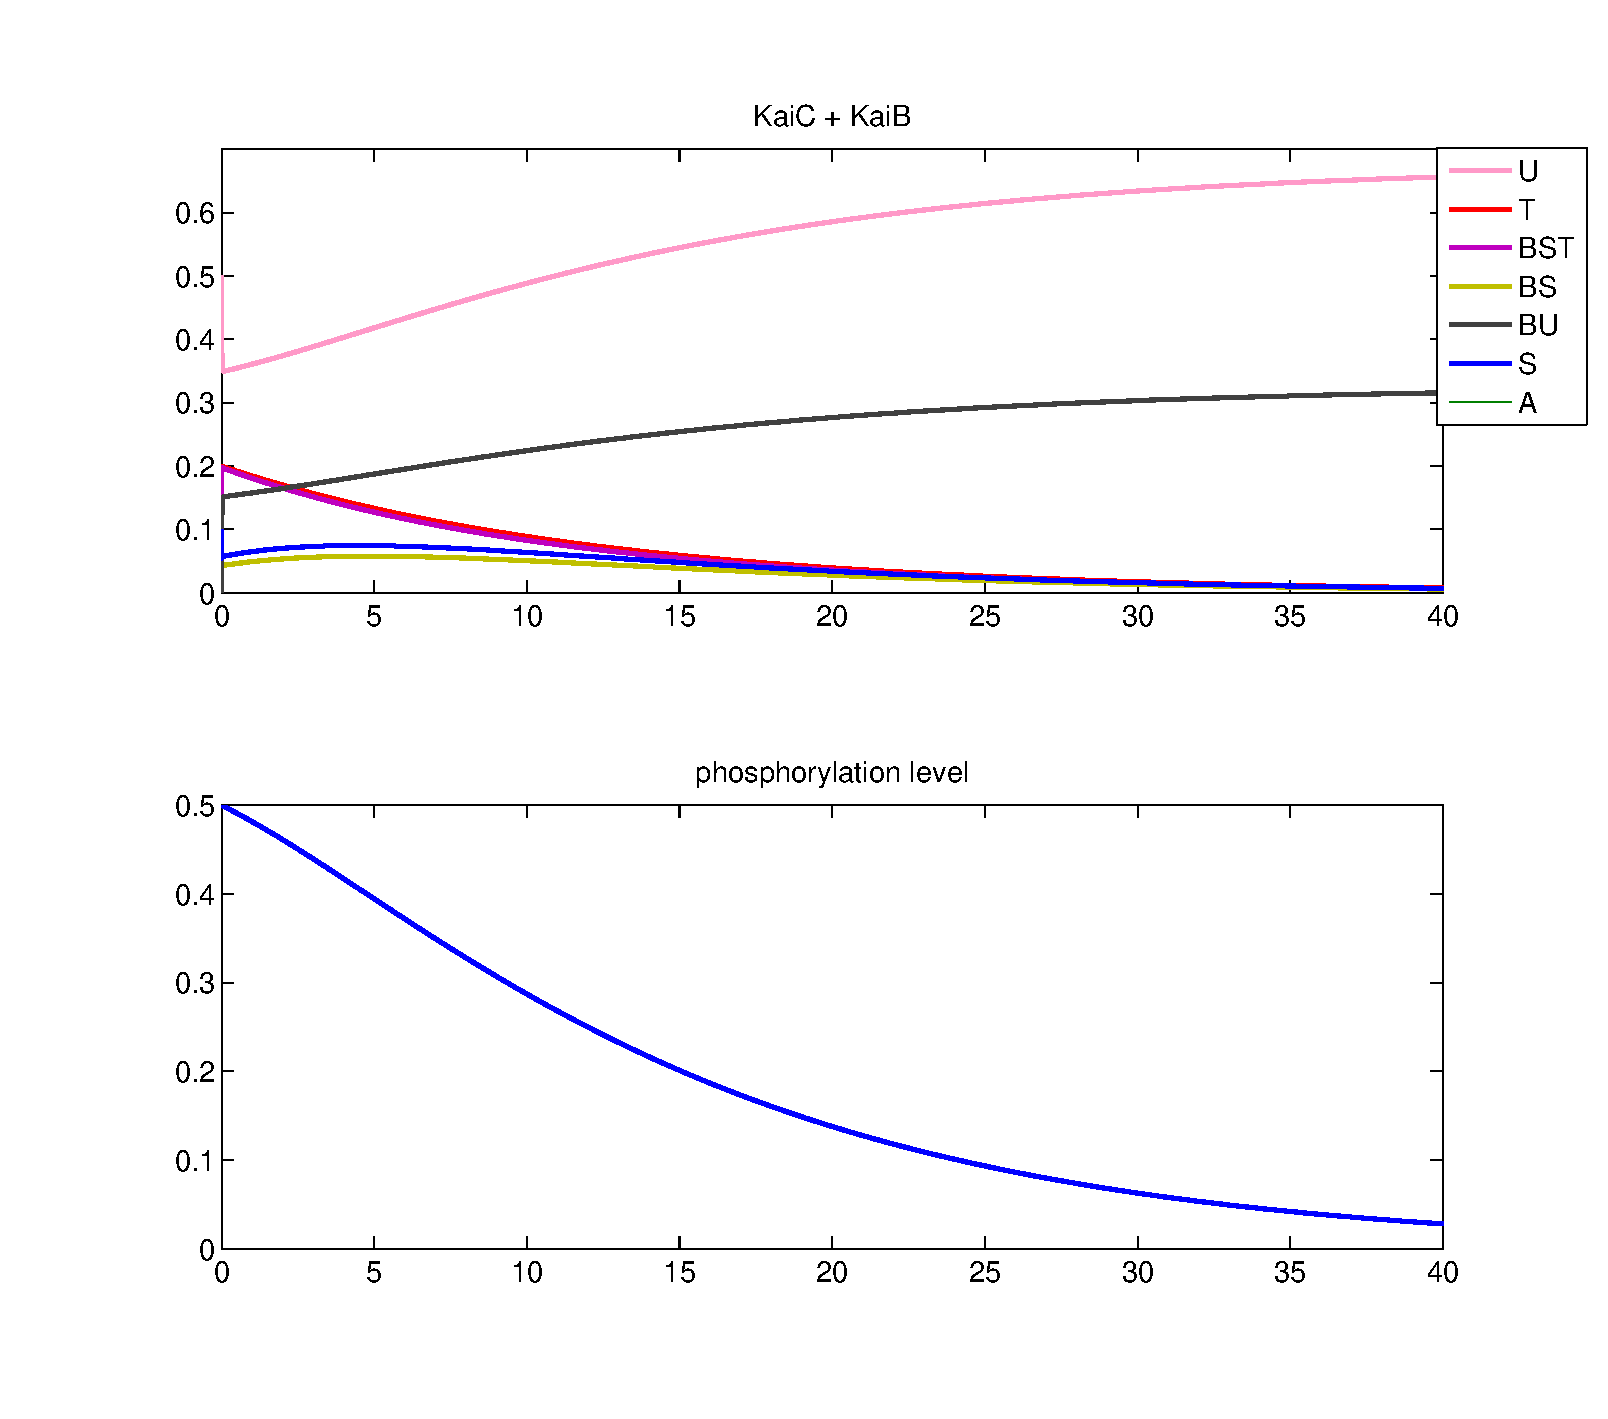
\includegraphics[scale=0.6]{B+C.eps}
\caption{\fontfamily{lmss}\selectfont Temporal profiles of different KaiC complexes as well as the overall phosphorylation level without any KaiA in the system. Initially KaiC is 50\% phosphorylated. Complexes that remain zero concentration due to initial conditions are omitted in the graph.}
\label{fig:B+C}
\end{figure}
It is also observed that when incubated with KaiA alone, the KaiC proteins will be driven to a highly phosphorylated state, consistent with results from \citet{Tamito2005}.
\begin{figure}[H]
\centering
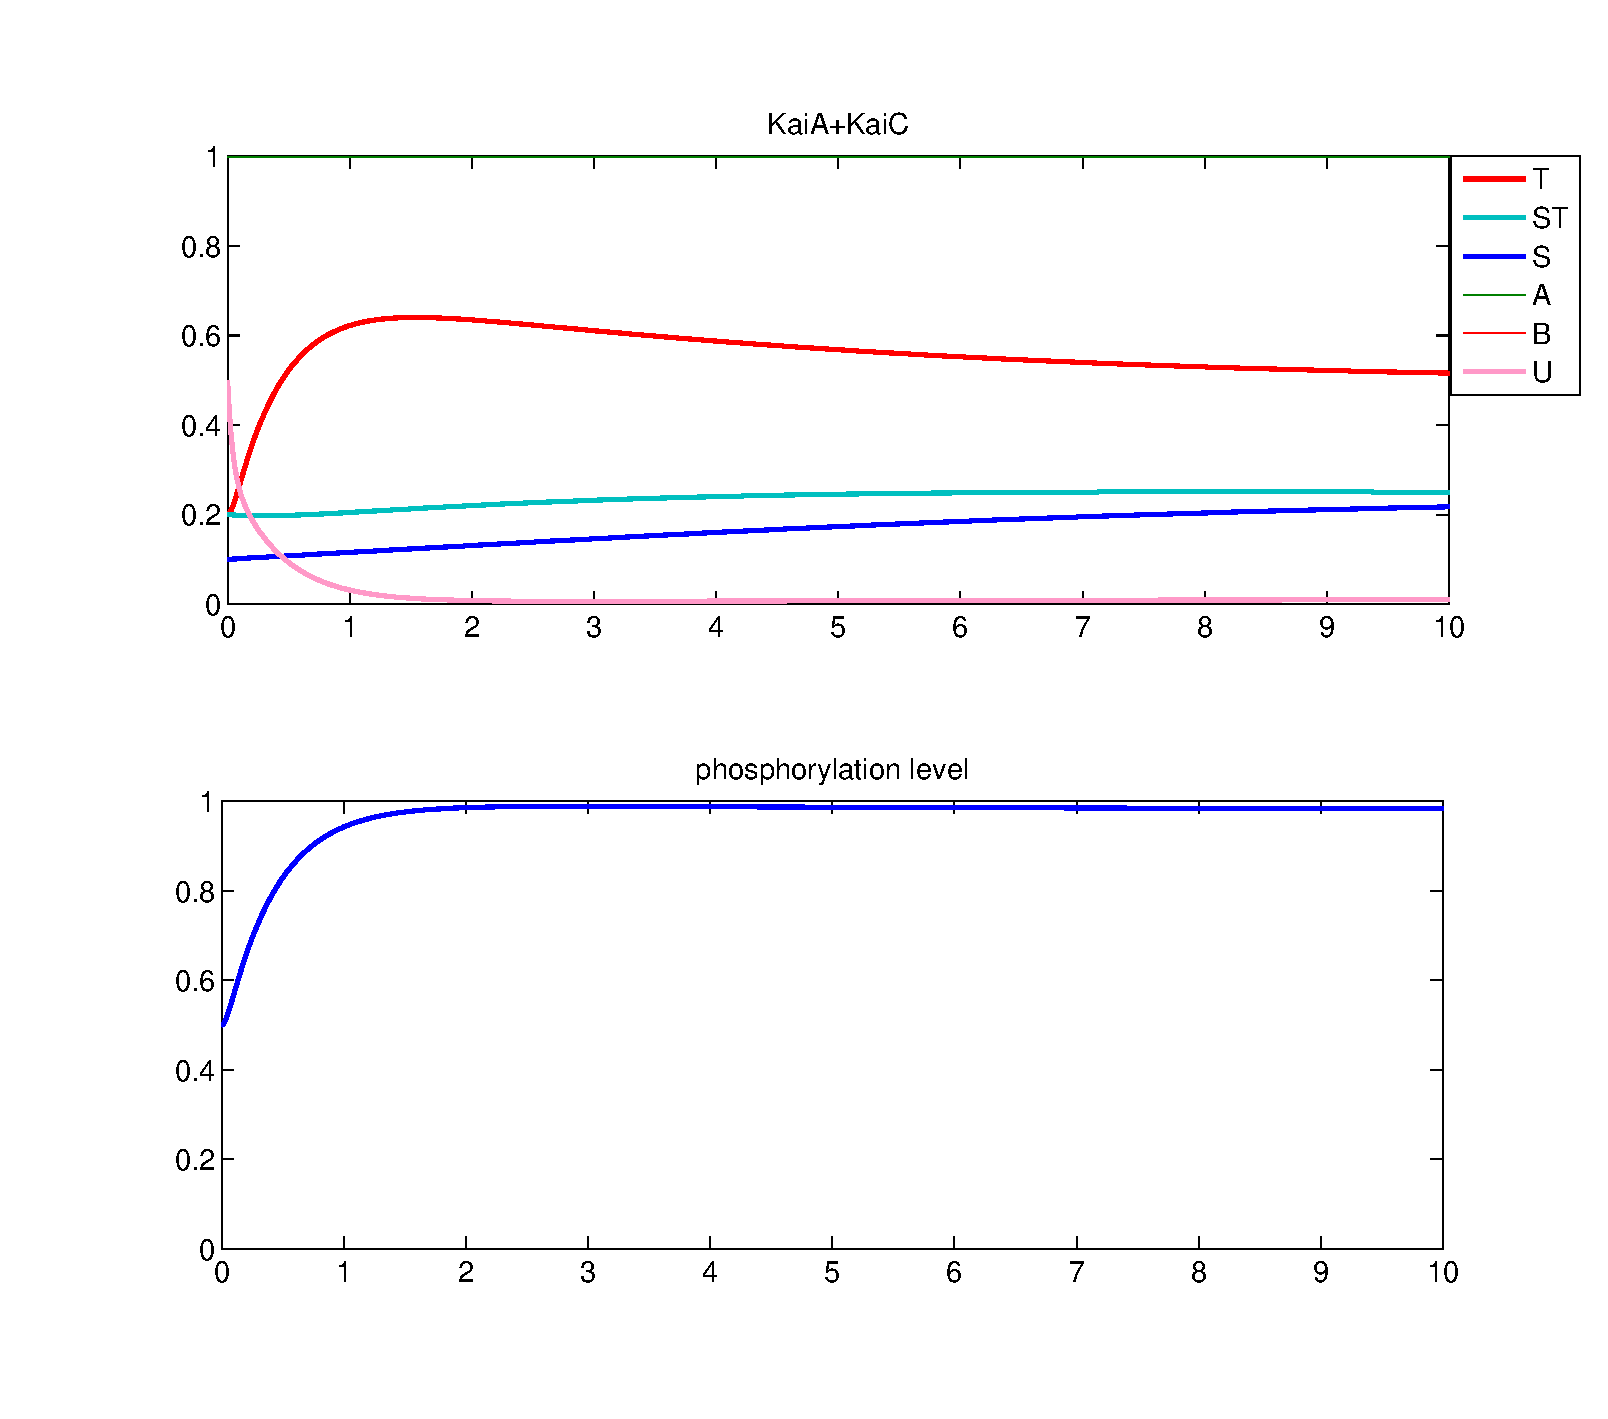
\includegraphics[scale=0.6]{A+C.eps}
\caption{\fontfamily{lmss}\selectfont Temporal profiles of different KaiC complexes as well as the overall phosphorylation level when KaiC is incubated with KaiA. The phosphorylation level reaches nearly 100\% within a short period of time. Initially KaiC is 50\% phosphorylated. Complexes that remain zero concentration due to initial conditions are omitted in the graph.}
\label{fig:A+C}
\end{figure}
\subsection{Temperature Compensation}




An important feature of circadian clocks, which is also true for most biological clocks, is their ability to remain at an almost unchanged period while environmental temperature can vary. This feature is known as 'temperature compensation', meaning that the effect of changes in temperature is compensated through an endogenous mechanism controlling the clock. A natural question to ask then is how this temperature-compensation is realized in circadian clocks, enabling robust regulations of biological behaviors essential to organisms.


Mathematical analysis (SI) shows that if all reactions respond to temperature changes in the same way, increasing temperature is equivalent to speeding up the time process. Therefore biological circadian clocks can not maintain a 24-h period at various temperature unless the reactions respond to temperature changes in a non-homogeneous way.

Different theories have been proposed to explain the mechanism behind temperature compensation, yet it still remains an active research area. \citet{hastings1957} propose a theory that certain reactions in a system is more sensitive to temperatures than others and some reactions can serve as temperature compensation elements, meaning that the effect of all reactions are balanced overall. \citet{lakin1991} also points out the possibility of increased amplitude while temperature increases, which serves as the counterpart of increased reaction rates. 



\subsection{Temperature Compensation}
An important feature of circadian clocks, which is also true for most biological clocks, is their ability to remain at an almost unchanged period while environmental temperature can vary. This feature is known as 'temperature compensation', meaning that the effect of changes in temperature is compensated through an endogenous mechanism controlling the clock. A natural question to ask then is how this temperature-compensation is realized in circadian clocks, enabling robust regulations of biological behaviors essential to organisms.
Different theories have been proposed to explain the mechanism behind temperature compensation, yet it still remains an active research area. \citet{hastings1957} propose a theory that certain reactions in a system is more sensitive to temperatures than others and some reactions can serve as temperature compensation elements, meaning that the effect of all reactions are balanced overall. \citet{lakin1991} also points out the possibility of increased amplitude while temperature increases, which serves as the counterpart of increased reaction rates. 



Here we show that our model generates oscillations that can be temperature compensated through a mechanism combining both theories in \citet{ruoff2004} and \citet{lakin1991}. To investigate the effects of varying reaction rates, we varied KaiA binding rates, KaiB binding rates as well as the KaiA-activated autokinase rate while keeping the rates of autokinase/phosphatase constants. In other words, we constrain the slow (de)phosphorylation rates to be rather  temperature-insensitive while allowing binding rates to vary. This assumption is supported by the experiments from \citet{Tamito2005}, where they demonstrated that  KaiC alone when incubated with ATP presents temperature-compensated autokinase/phosphatase activities.

We find that varying KaiB binding rates almost doesn't affect the period at all (Fig.\ref{fig:varyb}), possibly since these reactions are already fast enough and the period depend rather weakly on these rates. On the other hand, KaiA binding rates are much slower, which can have a more significant effect on the period. Our simulation on varying KaiA binding rates, however, still shows rather robust period keeping with less than 10\% change (Fig.\ref{fig:varya}). Moreover, we observe some interesting phase shift which can reflect a mechanism to adjust to sudden temperature change. Due to the phase shift effect, period seems to change more than it actually does. Therefore we also measure the period of each case and plot it against the varying rates (Fig.\ref{fig:temcompelmt}). Surprisingly, we find that KaiA binding can in fact serve as a temperature compensation element. As described in Hastings and Sweeney's theory, slowing these rates by a factor 1/2 or 1/5 actually shortens the period. In fact, we can explain this mechanism with theory from Lakin-Thomas et al. since the amplitude of the oscillation is increased when the reaction rates are increased (Fig.\ref{fig:ampvary}). We therefore conclude that the KaiA-activated autokinase reaction can also serve as a temperature compensation element since when temperature is decreased, period is shortened while amplitude is decreased (Fig.\ref{fig:varycat} and Fig. \ref{fig:tempcomp8}). 

In light of all the observations above, we predict that the mechanism to obtain temperature compensation in Cyanobacterial circadian clock falls into the linear theory by Peter Ruoff (\citet{ruoff1997}). Unlikely the argument in \citet{van2007}, we only assume that the (auto)dephosphorylation rate is naturally temperature compensated without engaging any KaiA or KaiB  (\citet{Tamito2005}), while we also explore the scenario where the (auto)phosphorylation rate does react to temperature with relatively low sensitivity.
 
All reactions in the system react to temperature changes with different sensitivity and a few reactions can serve as temperature compensation elements. According to Ruoff's theory, we expect to realize temperature compensation through balancing all reactions. Indeed, we investigate the corporate effect on period when increasing (un)binding rates with KaiB, (un)binding rates with KaiA, KaiA-activated phosphorylation rate and (auto)phosphorylation rate. 
First, we consider the case where phosphorylation rate $k_{dps}$ is also temperature compensated itself, and we find that the period remains constant while other reaction rates increase at least fourfold (Fig.\ref{fig:fixedperiod1}).



Further, we explore the case where we allow the phosphorylation rate $k_{ps}$ to have low temperature sensitivity while we still constrain the dephosphorylation rate $k_{dps}$ to be temperature-compensated. To reflect such low sensitivity, we assume that $k_{ps}$ increases only 20\% while other rates can increase by folds. Temperature compensation can still be achieved within a tolerance level (less than 4\% in Fig.\ref{fig:fixedperiod2}).

In both cases, different temperatures ($T_i$, $i=0,1,2,3$) is characterized by different reactions rates as Table. \ref{table:temperature}.


Although the assumption that the dephosphorylation rate is temperature-compensated has been supported by the experiments in \citet{Tamito2005}, the reasons behind such scheme remains unclear. There has been different theories proposed based on experimental results, among which is the result from \citet{kondo2012} where they found a transient increase in the amount of ATP during the KaiC autodephosphorylation process. They hypothesized that the KaiC dephosphorylation process can be decomposed into several biochemical reactions with the formation of ATP as an intermediate \citet{kondo2012}. Inspired by their work, here we propose a similar mechanism for the dephosphorylation process which can be incorporated into our model. We assume that a phosphoryl  


\begin{equation}
\begin{gathered}
\mathrm {ATP}\overset{ k_{1}}{\underset{k_{2}}{\rightleftarrows}} \mathrm { ADP\cdot Pi} \\
\mathrm {ST+ADP}\overset{ k_{3}}{\underset{k_{4}}{\rightleftarrows}} \mathrm {S + ATP} \\
\mathrm {S+ADP}\overset{ k_{5}}{\underset{k_{6}}{\rightleftarrows}} \mathrm{U + ATP} \\
\end{gathered}\label{eq:autodps}
\end{equation}

In our simulations, we first choose a parameter set that shows similar quantitative behavior as that in \citet{kondo2012} (Fig.\ref{fig:autodpsoriginal}). The initial conditions for the simulations are: 
\[[ATP/ADP]_{total}= 0.5106 \mu M,\; [ATP]= 0.0344*[ATP/ADP]_{total}, \]
\[ [C]_{total}=1.5\mu M,\; [U]=0.2*[C]_{total}, \; [S]=0.5*[C]_{total}, \; [ST]=0.3*[C]_{total} \] 


Then we vary the reaction rates individually to find out how each of them affects the dephosphorylation process (Table \ref{table:autodps}).  In the end, we find a balance among all rate changes such that temperature compensation can be achieved (Table \ref{table:autodps}), following the theory by \citet{hastings1957}. We indeed observe temperature compensation since the changes in the time scale of the resulted profile is much smaller than the changes in the reaction rates (Fig.\ref{fig:autodpstempcomp}). 



In conclusion, we propose the following mechanism for temperature compensation in Cyanobacterial circadian rhythm:
\begin{enumerate}
\item The dephosphorylation rate is temperature compensated itself without engaging KaiA or KaiB. We have also demonstrated how this can be realized through the balance of several decomposed reactions.
\item The (auto)phosphorylation rate has very low sensitivity to temperature: when temperature increases, the (auto)phosphorylation rate is first temperature-compensated and once the temperature enters a certain region, the reaction speeds up slowly.
\item The unbinding rate of KaiA to KaiC is rather sensitive to the temperature and serves as the main temperature compensation element. It counteracts the period shortening effect from increased phosphorylation rates.
\item KaiC (un)binds with KaiB fast enough so that even when the rates are increased several folds, there is no significant effect on the period.
\end{enumerate}

The proposed mechanism can be tested experimentally by manipulating the (un)binding power of KaiA to KaiC. We predict that if KaiA unbinds KaiC with a controlled rate despite temperature changes, then the temperature compensation is lost. Moreover, one can also test if temperature compensation will be preserved when the (un)binding power of KaiB to KaiC is weakened experimentally. 


Mathematical analysis shows that if all reactions respond to temperature changes in the same way, increasing temperature is equivalent to speeding up the time process. Therefore biological circadian clocks can not maintain a 24-h period at various temperature unless the reactions respond to temperature changes in a non-homogeneous way.


It is known that most reactions happen when two molecules collide with enough energy (sometimes called activation energy) and when they are head in some appropriate direction. We also know from statistical mechanics that most reaction rates follows the Arrhenius relation $k=A\exp(-E/RT)$, where $E$ is the activation energy, $R$ is the gas constant and $T$ is the absolute temperature. In other words, most reaction rates strongly depend on temperature.

In a biological system, we consider all reactions $R_i$'s and the corresponding rate constants $k_i$'s, indexed by $i$. Then the reaction rates depend on temperature following the Arrhenius relation $k_i=A_i\; e^{-E_i/RT}$.

Suppose the differential equations describing the dynamics of the system are: 
\begin{equation}\label{eq:original}
\frac{d X_j}{dt} = f_j(\overrightarrow{X})  \quad j=1,2,...,N
\end{equation} 
where $X_j$'s are the state variables and each $f_j$ is a linear combination of terms in the form $k_iX_1^{a_1}X_2^{a_2}\cdots X_N^{a_N}$ following the law of mass action. 
If all reactions speed up at the same rate when the temperature increases, can the system be temperature-compensated? To answer this question, we assume that all $k_i$'s are increased by the same factor $p$, then the right hand side of each equation is also multiplied by a factor $p$ since the new linear combination term becomes $p*k_iX_1^{a_1}X_2^{a_2}\cdots X_N^{a_N}$:
\[
\frac{d X_j}{dt} = p*f_j(\overrightarrow{X})  \quad j=1,2,...,N 
\]
After a change of variable/scaling of time $\tilde{t}=p*t$, we can recover the system into the same form as Eq.\ref{eq:original}.
\begin{equation}
 \frac{d X_j}{d\tilde{t}} = f_j(\overrightarrow{X})  \quad j=1,2,...,N 
\end{equation}

The linear theory has been developed mathematically in many papers by Peter Ruoff and was summarized in a recent book chapter \citet{ruoff2004}. He assumed that the period $\tau$  of a biological clock can be written as a complicated yet differentiable function of all reaction rates:
\begin{equation}
\tau=F(k_1,k_2,\cdots ,k_M)
\end{equation}

Denoting temperature by $T$ again, the rate of change of period length with respect to temperature can then be computed using chain rule from  basic calculus:
\begin{equation}
\begin{split}\label{eq:rateofchange}
\frac{\partial \tau}{\partial T} &= \sum_i \frac{\partial F(k_1,k_2,\cdots ,k_M)}{\partial k_i} \frac{\partial k_i}{\partial T}\\
&=\sum_i \frac{\partial F(k_1,k_2,\cdots ,k_M)}{\partial k_i} A_i\;e^{-E_i/RT}(\frac{E_i}{RT^2})\\
&=\sum_i \frac{\partial F(k_1,k_2,\cdots ,k_M)}{\partial k_i} k_i (\frac{E_i}{RT^2})\\
&=\sum_i \frac{\partial F(k_1,k_2,\cdots ,k_M)}{\partial \ln k_i}  (\frac{E_i}{RT^2})
\end{split}
\end{equation}
where in the second line, $\frac{\partial k_i}{\partial T}$ is computed according to the Arrhenius relation $k_i=A_i\; e^{-E_i/RT}$.

Multiplying $\frac{1}{\tau}$ on both sides of the last equation in Eq.\ref{eq:rateofchange} and abbreviating $F(k_1,k_2,\cdots ,k_M)$ as $F$ we have:
\begin{equation*}
\frac{\partial \tau}{\partial T}\frac{1}{\tau}= \sum_i \frac{\partial F}{\partial \ln k_i} \frac{1}{F}  \frac{E_i}{RT^2}, 
\end{equation*}
which can be rewritten as
\begin{equation}\label{eq:integral}
\frac{\partial \ln \tau}{\partial T}= \sum_i \frac{\partial \ln F}{\partial \ln k_i} \frac{E_i}{RT^2}. 
\end{equation}

Since $\tau\neq 0$, we have
\[ \frac{\partial \tau}{\partial T} =0 \iff \frac{\partial \ln \tau}{\partial T}=0 \iff \sum_i \frac{\partial \ln F}{\partial \ln k_i} \frac{E_i}{RT^2}=0. \forall T\] 
Multiplying $RT^2$ on both sides of the equation and we obtain the  condition for temperature compensation:

\begin{equation}\label{eq:balance}
\sum_i \frac{\partial \ln  F}{\partial \ln k_i} E_i = 0
\end{equation}

Now we define the sensitivity of period to each reaction as below:
\[ \beta_i=\frac{\partial \ln  F}{\partial \ln k_i}\]

At a given temperature, we have $\beta_i>0$  for reactions that contribute positively to the period length and $\beta_i< 0$ otherwise. Temperature compensation is then realized through a weighted balance among all the sensitivity coefficients $\beta_i$'s. Therefore the Ruoff's theory is indeed  a more rigorous mathematical extension from \citet{hastings1957}. 

Under linear assumption by Ruoff, $\beta_i$'s are constants. Therefore we can integrate Eq.\ref{eq:integral} to obtain a relationship between $\tau$ and $T$:
\begin{equation}
\begin{split}
\int d\ln \tau&=\sum_i \beta_i E_i \int \frac{dT}{RT^2}\\
\ln \tau &= -\frac{1}{RT}\sum_i \beta_i E_i +C\\
\tau &= \tau_0 \exp\left({-\frac{\sum_i \beta_i E_i}{RT}}\right)
\end{split}
\end{equation}

Ruoff argues that by choosing $E_i$'s properly, the balance condition Eq.\ref{eq:balance}   can be achieved and  this  tuning is realized through evolution. In practice, one can also find potential temperature compensation elements (reactions satisfying $\frac{\partial \ln  F}{\partial \ln k_i}>0$) by investigating how the the period changes when each reaction rate is increased. Once such elements are identified, temperature compensation can be realized in the system by tuning the factors by which reaction rates speed up when temperature increases (equivalent to tuning $E_i$'s).

% We find that varying KaiB binding rates almost doesn't affect the period at all (Fig.\ref{fig:varyb}), possibly since these reactions are already fast enough and the period depend rather weakly on these rates. 


\begin{figure}
\centering
\begin{subfigure}{0.8\textwidth}
\centering
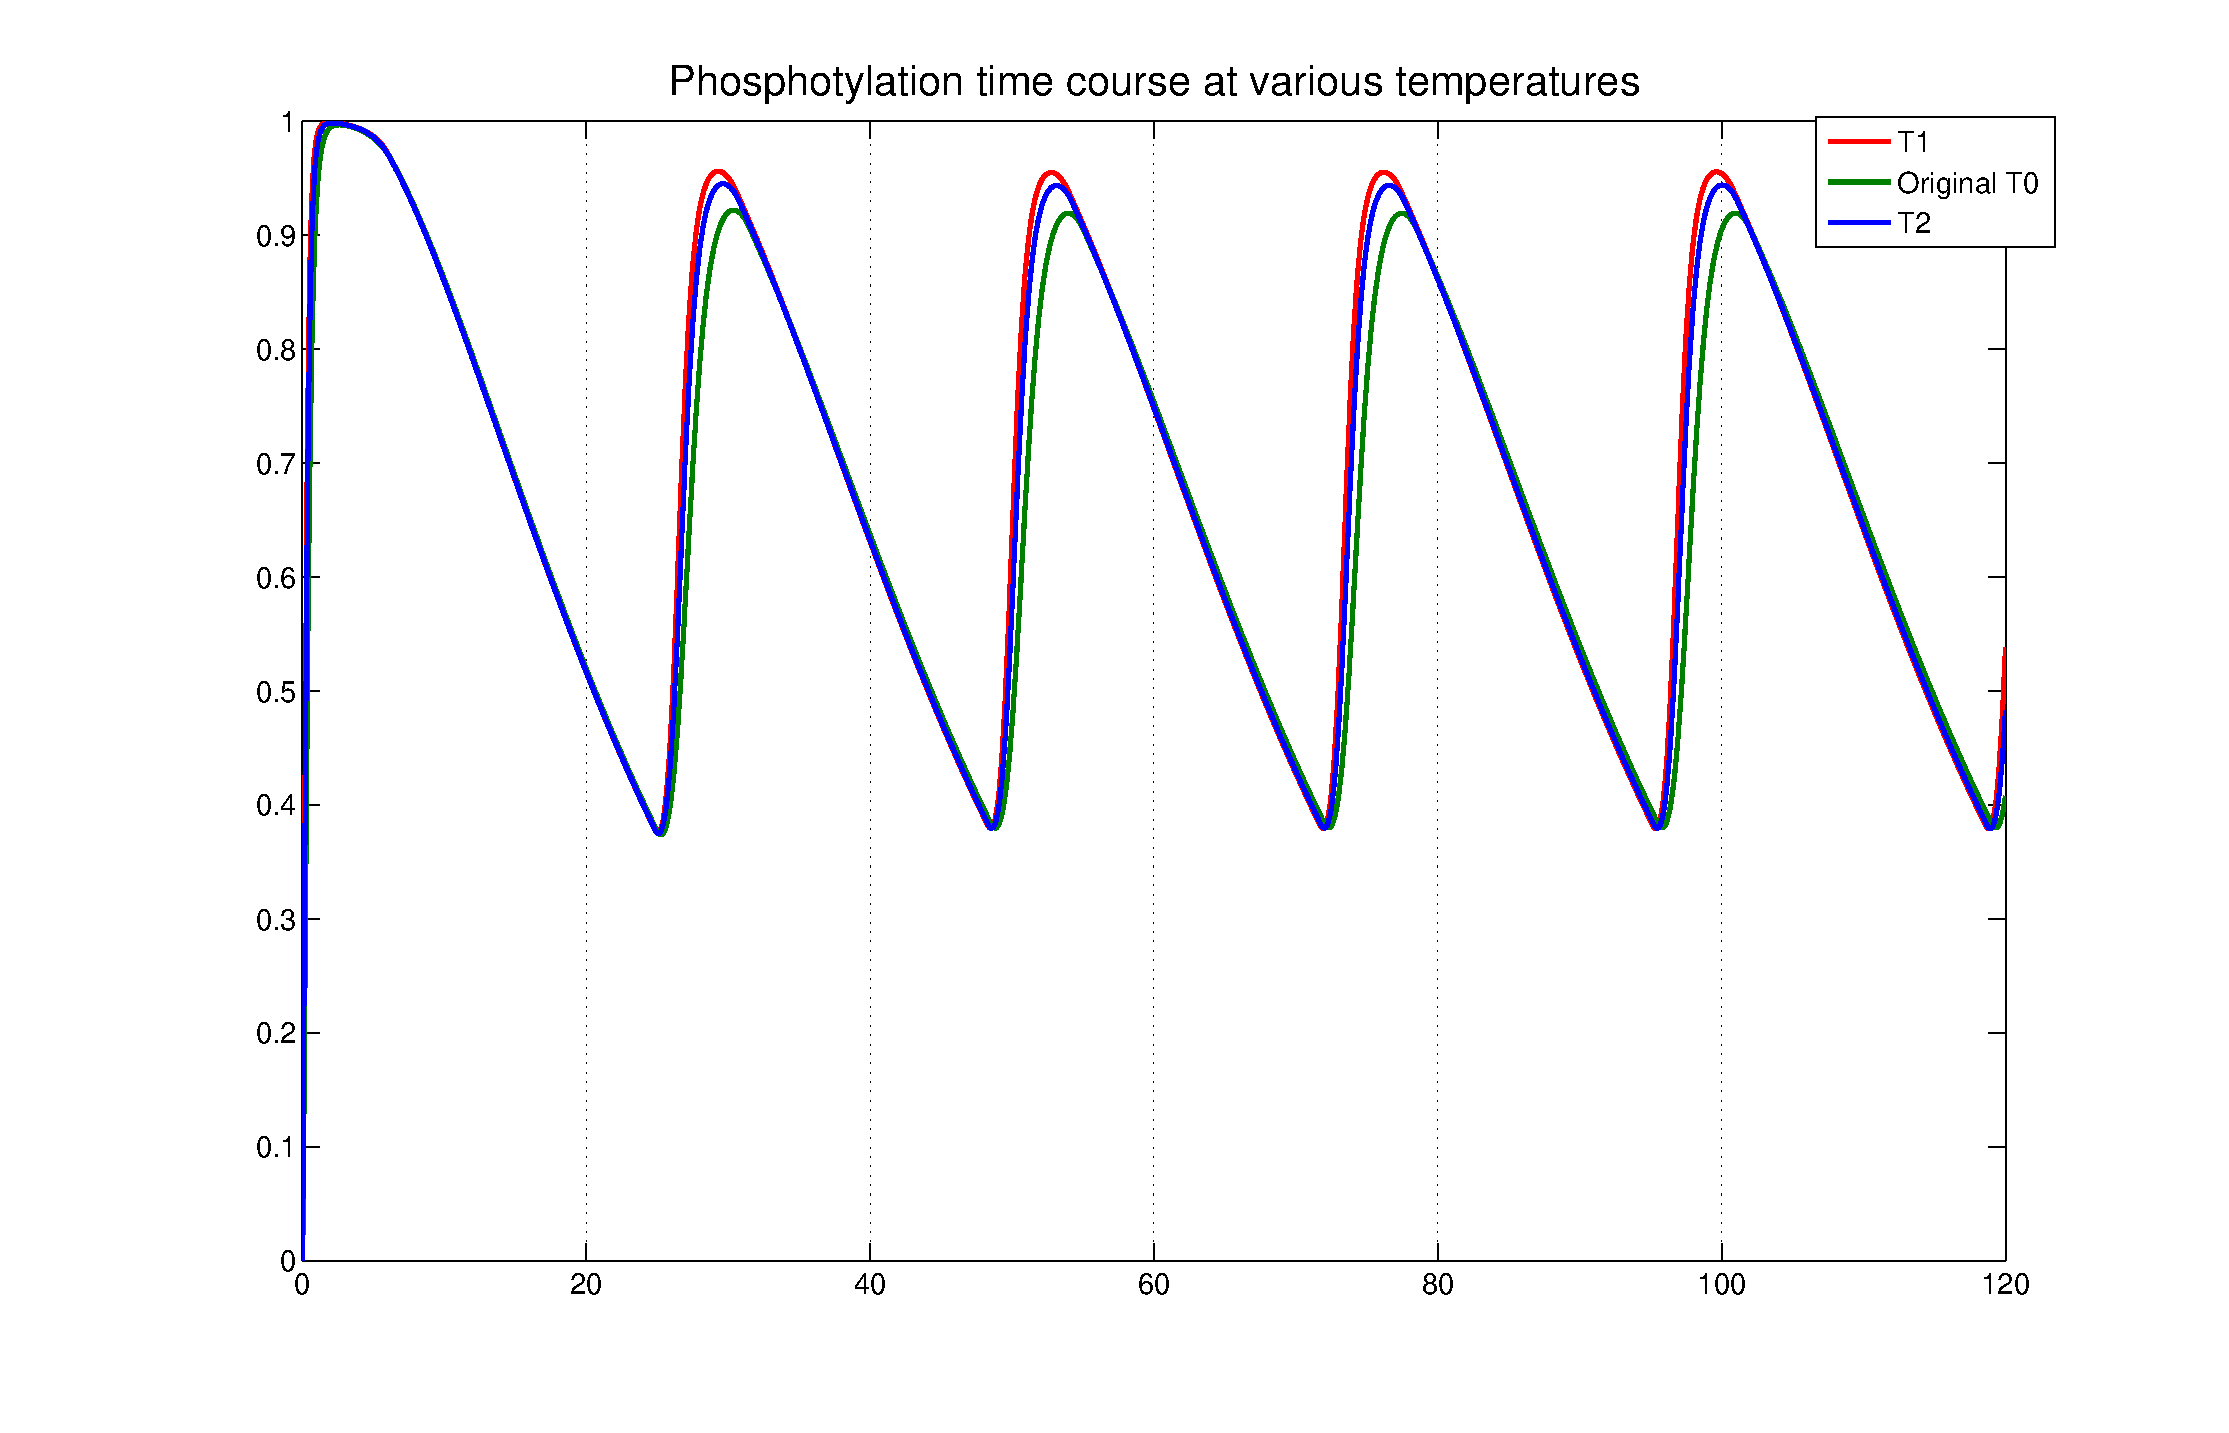
\includegraphics[scale=0.3]{fixedperiod1.eps}
\caption{\fontfamily{lmss}\selectfont Temperature Compensation realized by balancing reactions. Period remains at 23.54h for all three temperatures with some natural phase shift. Time course curves overlap strongly for all three temperatures, indicating the robustness of this mechanism.}\label{fig:fixedperiod1}
\end{subfigure}
\begin{subfigure}{0.8\textwidth}
\centering
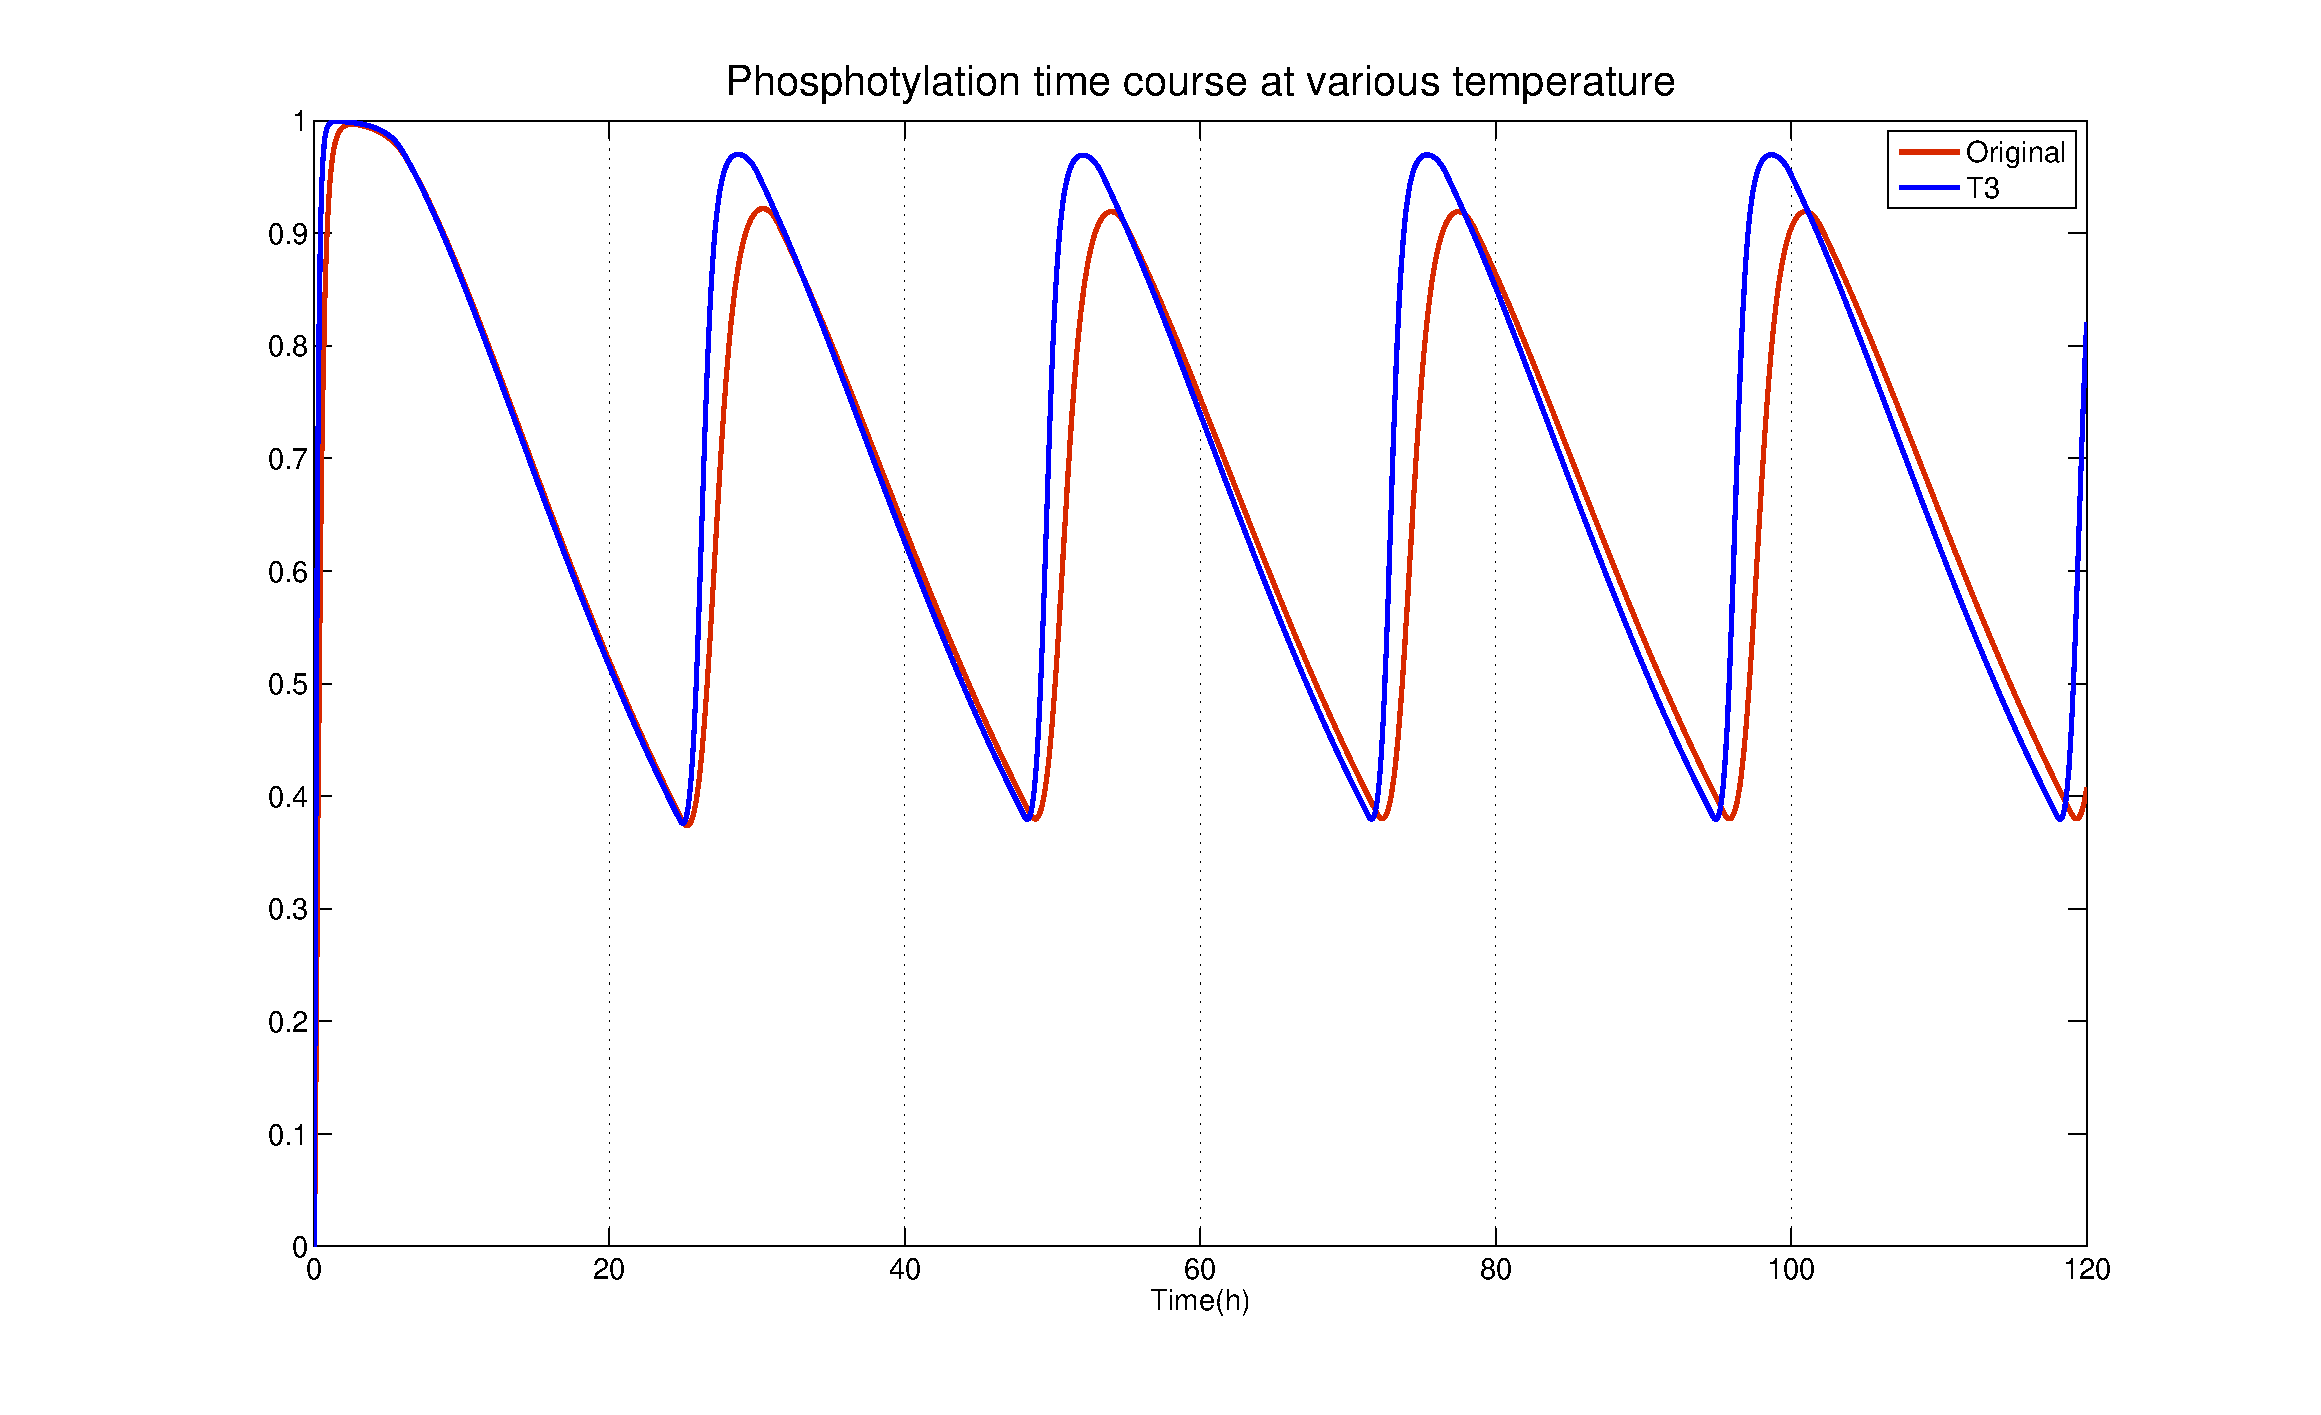
\includegraphics[scale=0.3]{fixedperiod2.eps}
\caption{\fontfamily{lmss}\selectfont The original period (23.54h at $T_0$) shortens less than 4\% when temperature increases (22.69h at $T_3$). }\label{fig:fixedperiod2}
\end{subfigure}
\caption{Temperature compensation}
\end{figure}


\begin{table} 
\centering
 \begin{tabular}{||c||c c c c c c | c||} 
 \hline
 & \multicolumn{6}{|c|}{Ratio of rates to original value ($T_0$)} & \\
 \hline
 & $K_{ps}$ & $K_{a}$ & $K_b$ & $K_f$ & $K_i^{\mathrm {on}}$/$K_i^{\mathrm {off}}$ & $K_{dps}$ & Period\\ [0.5ex] 
 \hline\hline
 $T_0$ & 1 & 1 & 1 & 1  & 1& 1 & 23.54\\ 
 \hline
 $T_1$ & 1 & 2 & 6 & 2 & 2 & 1& 23.54\\
 \hline
 $T_2$ & 1 & 4 & 27.5 & 5 & 5& 1&23.53\\
 \hline
 $T_3$ & 1.2 & 4 & 25 & 6 & 8 & 1 & 22.69\\[1ex] 
 \hline
\end{tabular}
\caption{\fontfamily{lmss}\selectfont A table of how reactions are balanced at each hypothetical temperature. The notation of reaction rates are the same as in Eq \ref{eq:full}.}
\label{table:temperature}
\end{table}

\begin{figure}
\centering
\begin{subfigure}{0.45\textwidth }
\centering
\includegraphics[height=7cm,width=9cm]{kondo2012.jpg}
\end{subfigure}
\begin{subfigure}{0.45\textwidth }
\centering
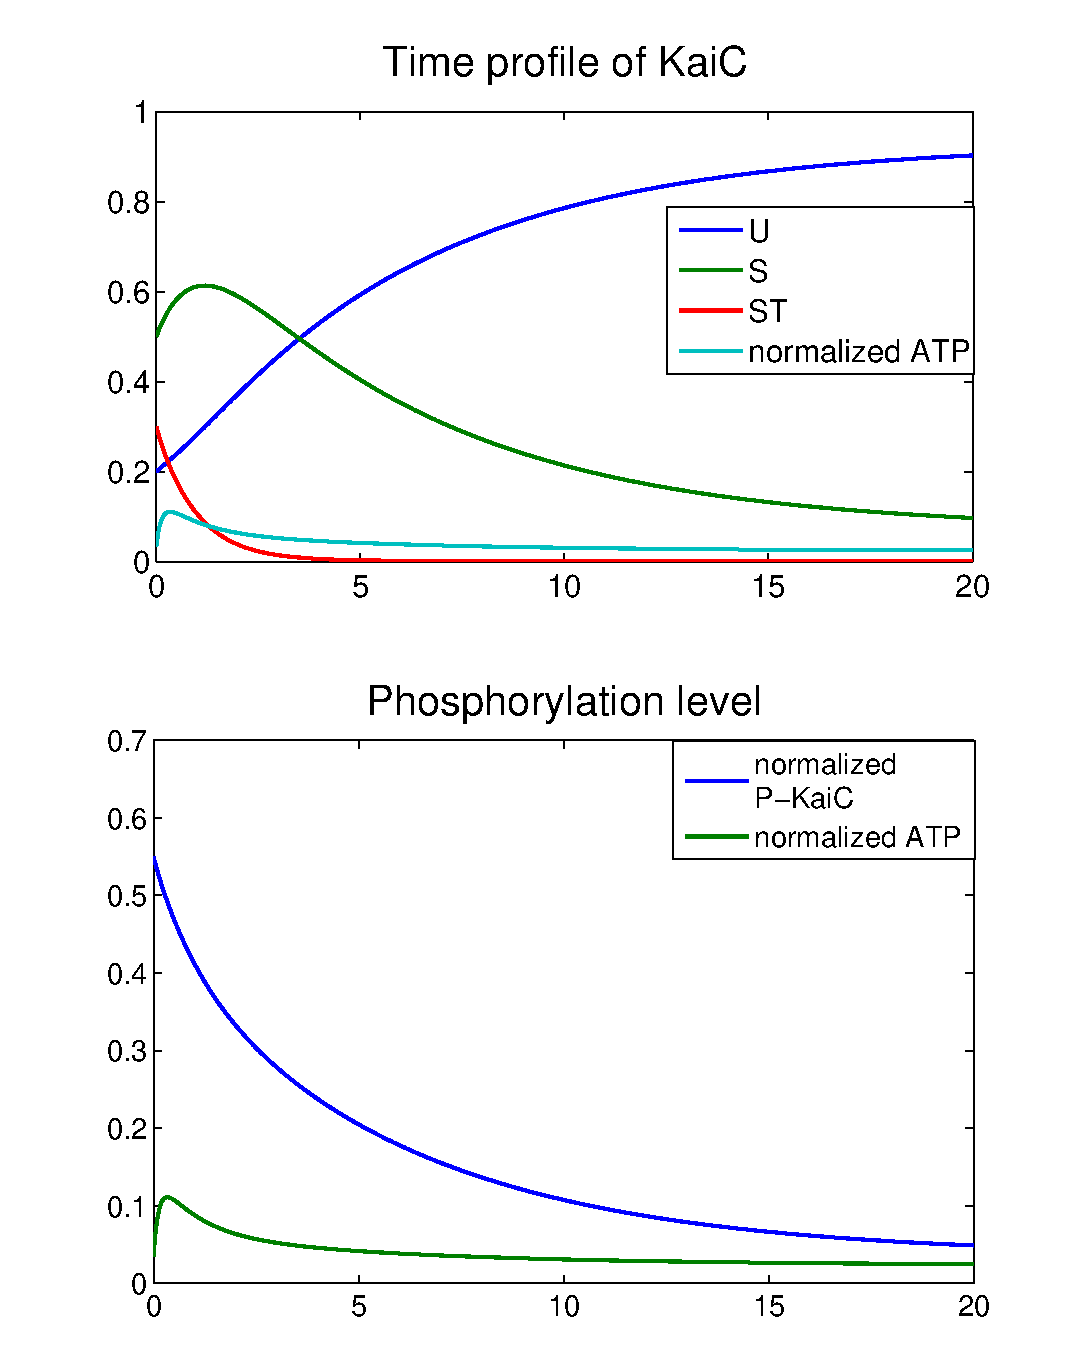
\includegraphics[scale=0.5]{autodps5original.eps}
\end{subfigure}
\caption{\fontfamily{lmss}\selectfont Left panel is the experimental result from \citet{kondo2012} where there is a transient ATP increase and dephosphorylation reaches near completion within 18h. Right panels are the simulation results from our model Eq.\ref{eq:autodps} with parameters from Table \ref{table:autodps}. We also observe the transient ATP increase at the beginning and the dephosphorylation reaches near completion in 20h. }\label{fig:autodpsoriginal}
\end{figure}

\begin{figure}
\centering
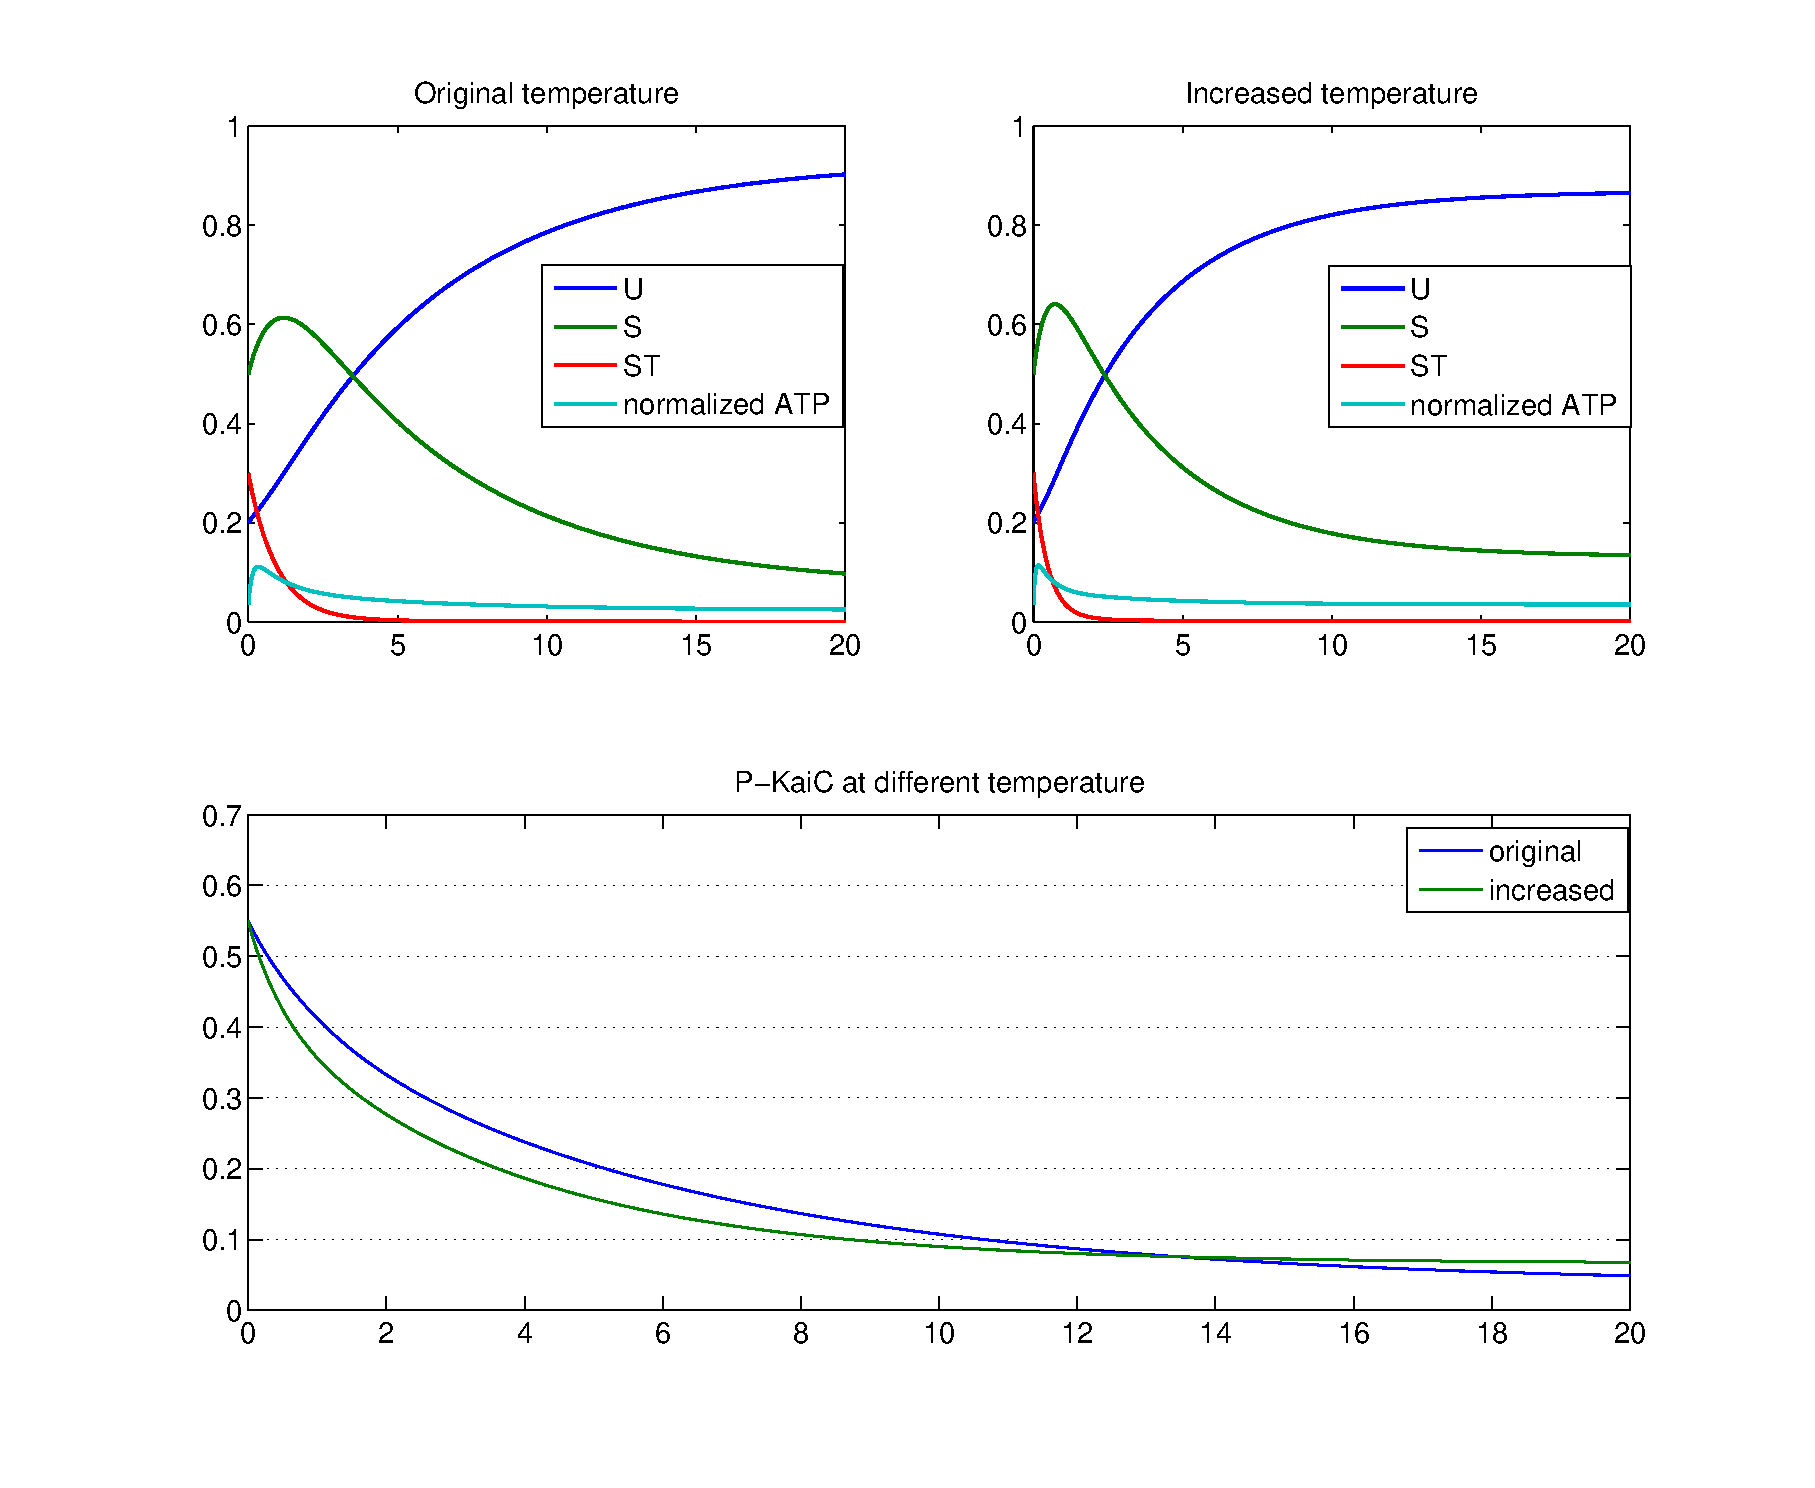
\includegraphics[scale=0.6]{autodps5tempcompfig9.eps}
\caption{\fontfamily{lmss}\selectfont Top panel are the simulated KaiC temporal files at different temperatures with the same initial conditions as in Fig. \ref{fig:autodpsoriginal}. All concentrations are normalized. The parameters corresponding to the original and increased temperature are in Table \ref{table:autodps}. Bottom panel compares the phosphorylation levels of KaiC at two different temperatures. Although the curves do not overlap completely, the differences between them are small enough compare to the rate changes. }\label{fig:autodpstempcomp}
\end{figure}




\begin{table}
\centering
 \begin{tabular}{||c|| c c c c c c |} 
 \hline
 Temperature/Rates & $k_1 (h^{-1})$ & $k_2(h^{-1})$ & $k_3(M^{-1}h^{-1})$ & $k_4(M^{-1}h^{-1})$ & $k_5(M^{-1}h^{-1})$ & $k_6(M^{-1}h^{-1})$ \\ [0.5ex] 
 \hline\hline
 Original & 6.4201 & 0.1538 & 2.3317 & 0.1942  &0.3641 & 1.1485 \\ 
 \hline
 Increased & 6.4201*2 & 0.1538*3.5 & 2.3317*2 & 0.1942*3  &0.3641*1.5 & 1.1485*2\\
 \hline
 Effect when increased &  +  & - & + & = & + & -\\[0.5ex]
 \hline
\end{tabular}
\caption{\fontfamily{lmss}\selectfont The first two rows show the parameters we use for the corresponding simulations. The last row shows how increasing each reaction rates affects the dephosphorylation process. '+' : the process is faster when the rate increases; '-': the process is slower when the rate increases; '=': the process remains almost the same when the rate increases.}
\label{table:autodps}
\end{table}


\begin{figure}[H]
\centering
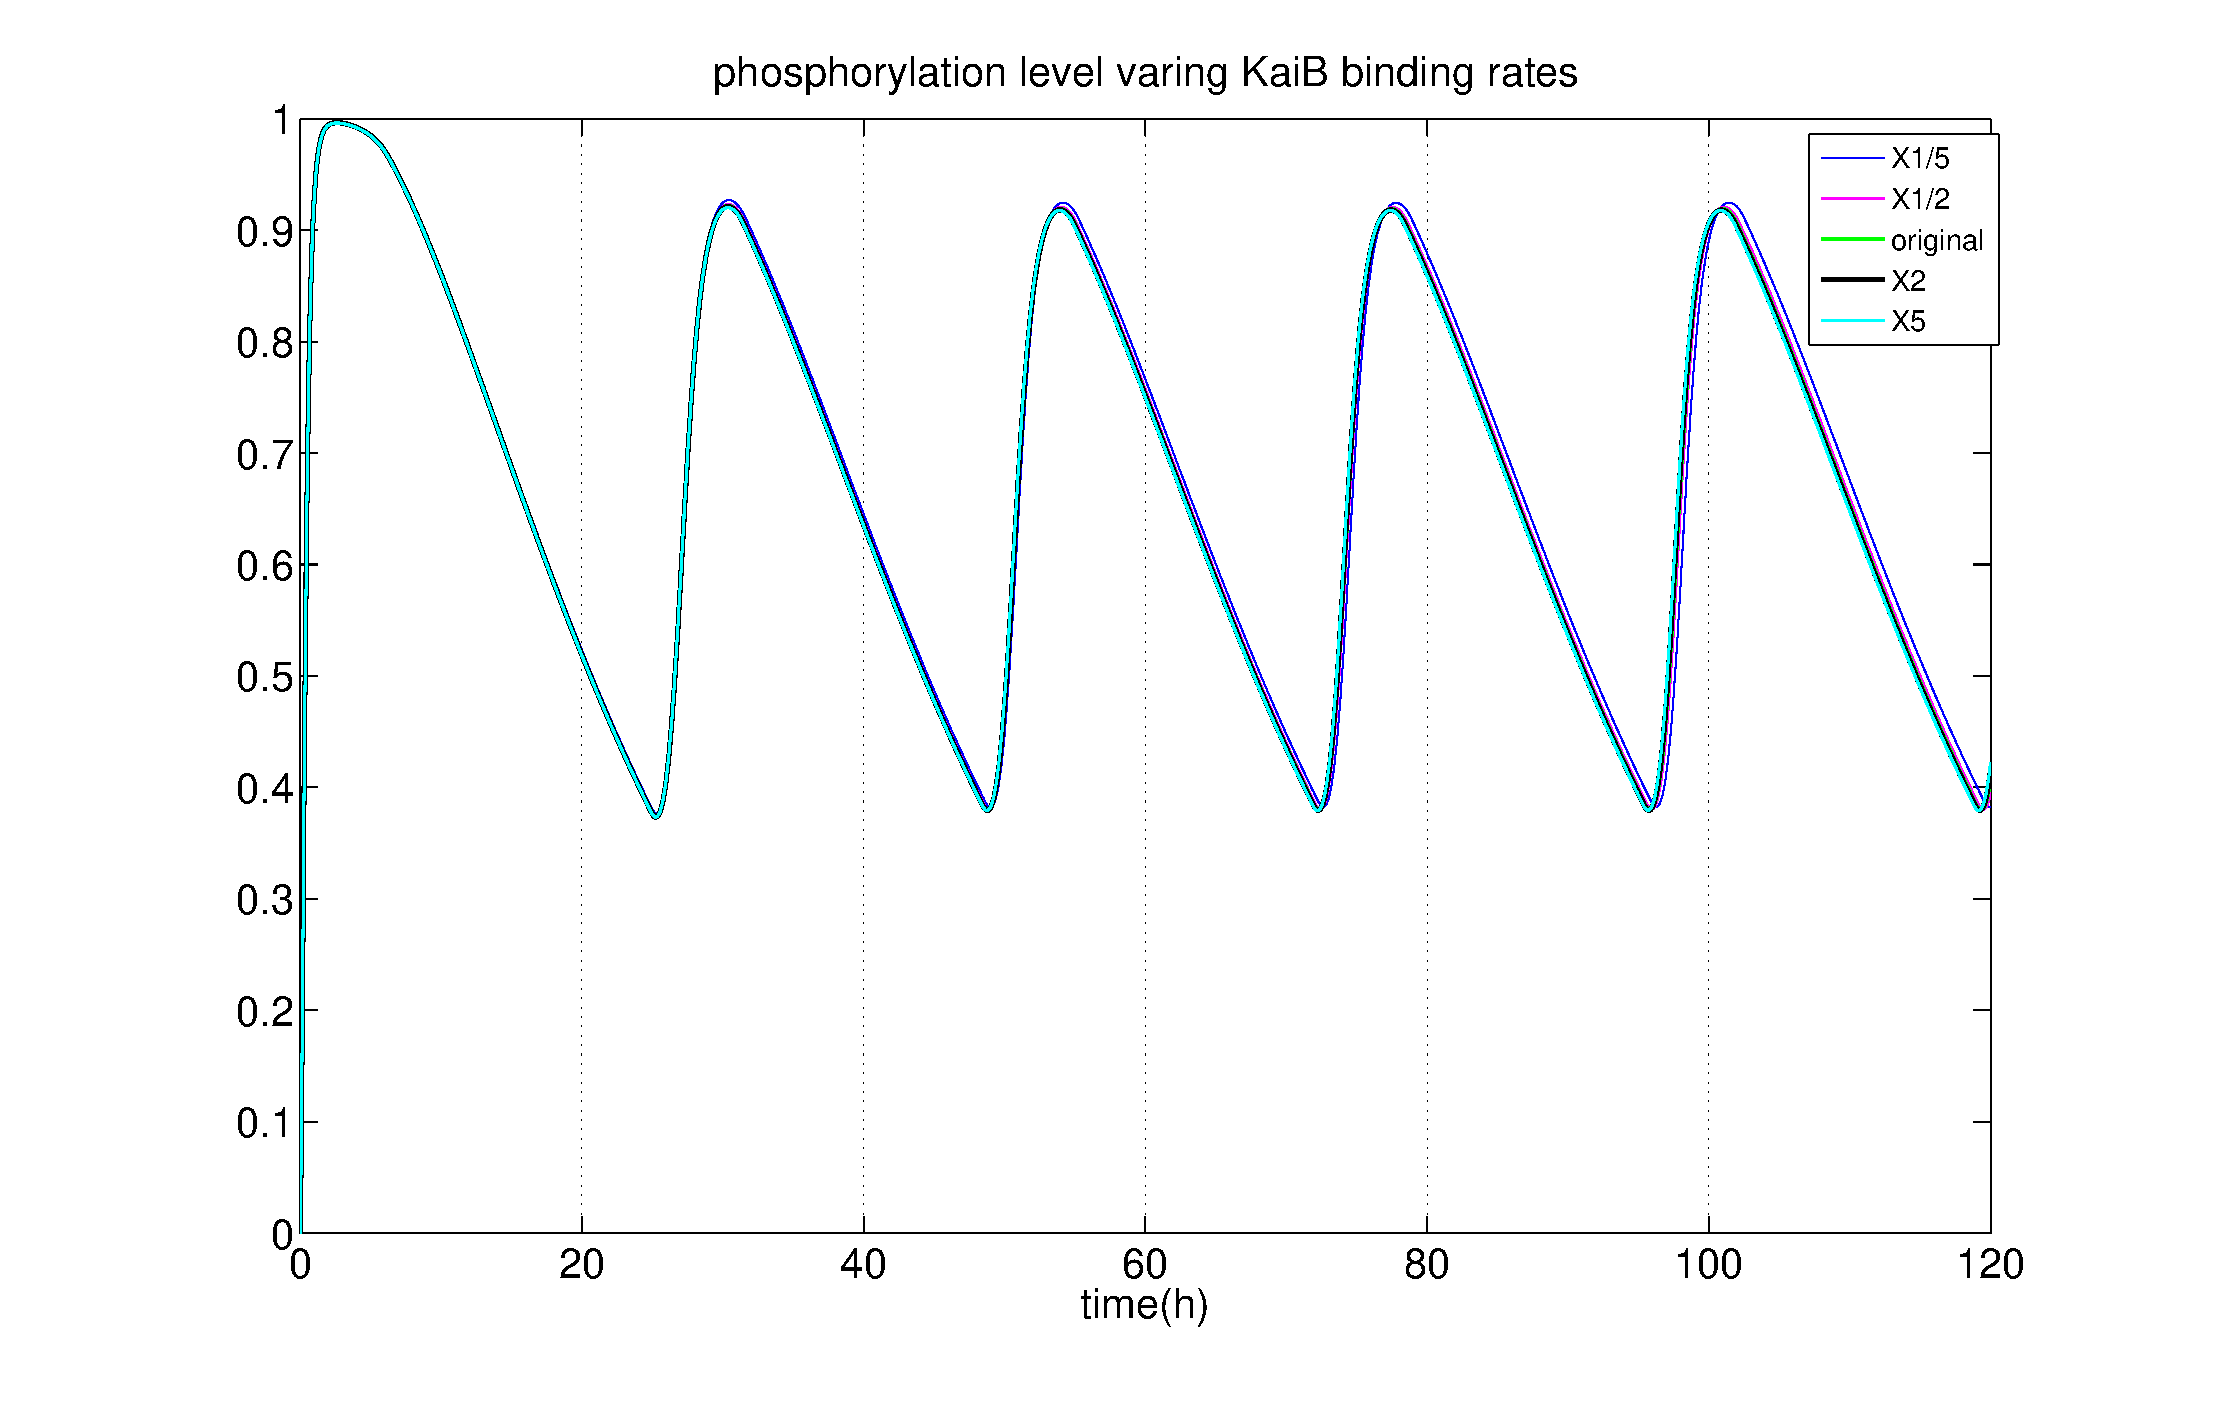
\includegraphics[scale=0.45]{tempcomp1.eps}
\caption{\fontfamily{lmss}\selectfont When KaiB binding rates are varied, the period is almost unchanged and ranges from 23.4h to 23.7h.}\label{fig:varyb}
\end{figure}

% On the other hand, KaiA binding rates are much slower, which can have a more significant effect on the period. Our simulation on varying KaiA binding rates, however, still shows rather robust period keeping with less than 10\% change (Fig.\ref{fig:varya}). Moreover, we observe some interesting phase shift which can reflect a mechanism to adjust to sudden temperature change. 




\begin{figure}[H]
\centering
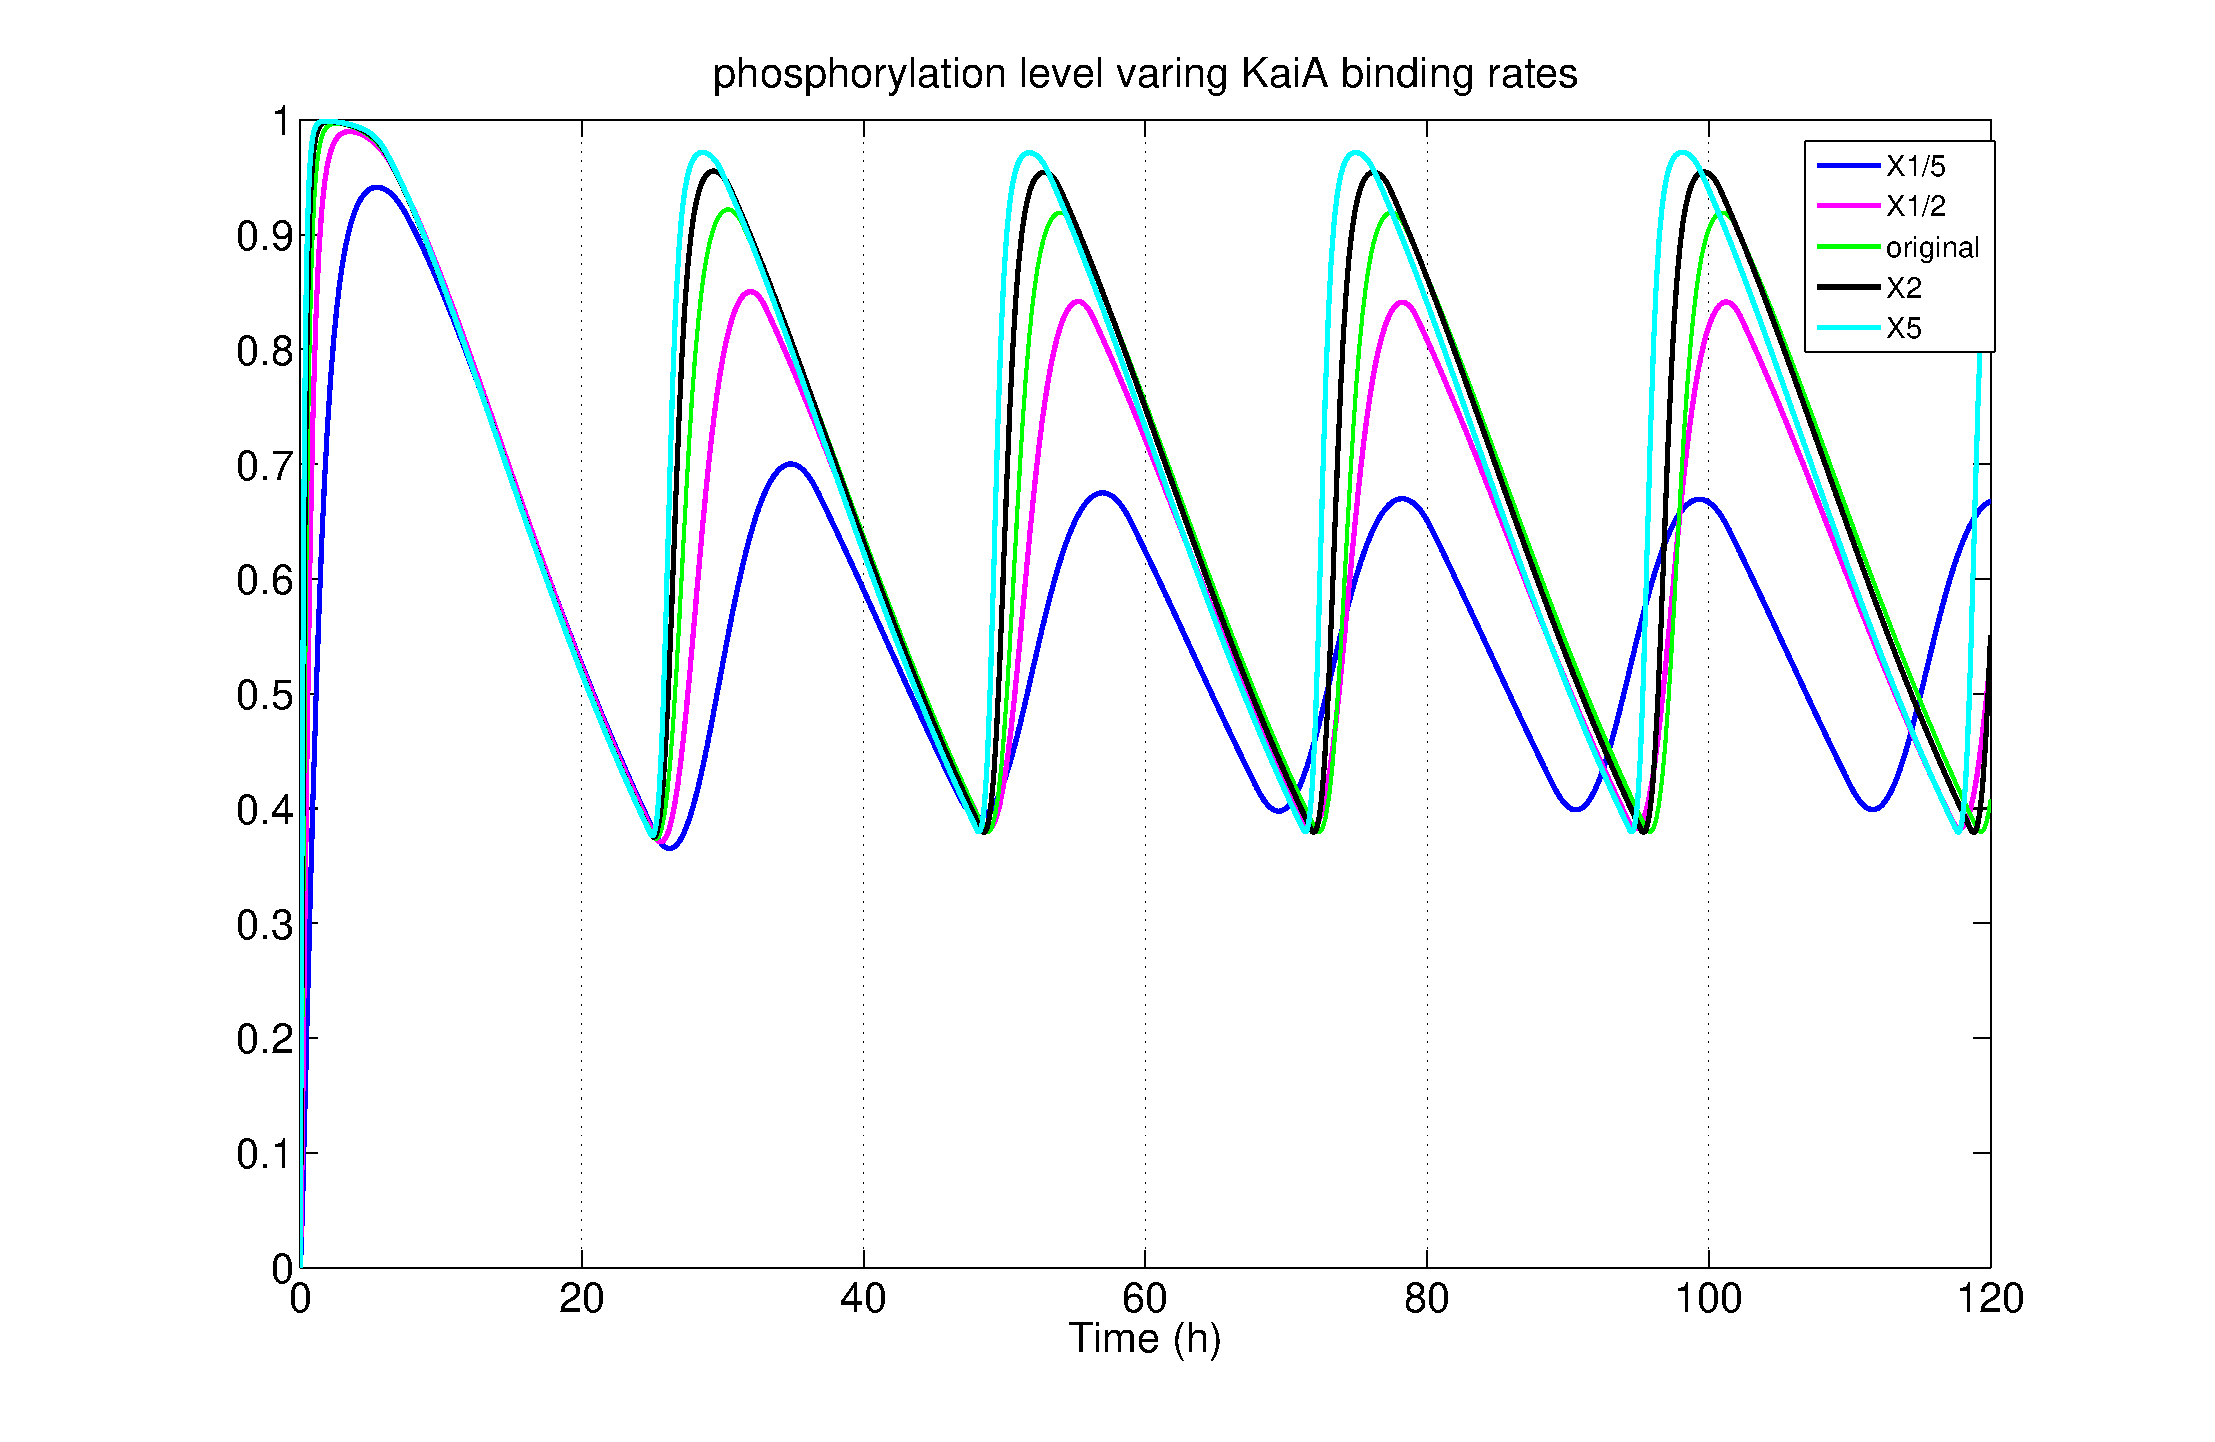
\includegraphics[scale=0.45]{tempcomp2.eps}
\caption{\fontfamily{lmss}\selectfont Period change is within 10\% (21.08h to 23.56h) and phase shift can be observed.}\label{fig:varya}
\end{figure}
% Due to the phase shift effect, period seems to change more than it actually does. Therefore we also measure the period of each case and plot it against the varying rates (Fig.\ref{fig:temcompelmt}). Surprisingly, we find that KaiA binding can in fact serve as a temperature compensation element. As described in Hastings and Sweeney's theory, slowing these rates by a factor 1/2 or 1/5 actually shortens the period. 

\begin{figure}[H]
\centering
\includegraphics[scale=0.4]{tempcomp6.eps}
\caption{\fontfamily{lmss}\selectfont Period is optimized at a roughly 24h length. Lowering the rates by a factor 1/2 or 1/5 results in a shorter period.}\label{fig:temcompelmt}
\end{figure}
% In fact, we can explain this mechanism with theory from Lakin-Thomas et al. since the amplitude of the oscillation is increased when the reaction rates are increased (Fig.\ref{fig:ampvary}). 

\begin{figure}[H]
\centering
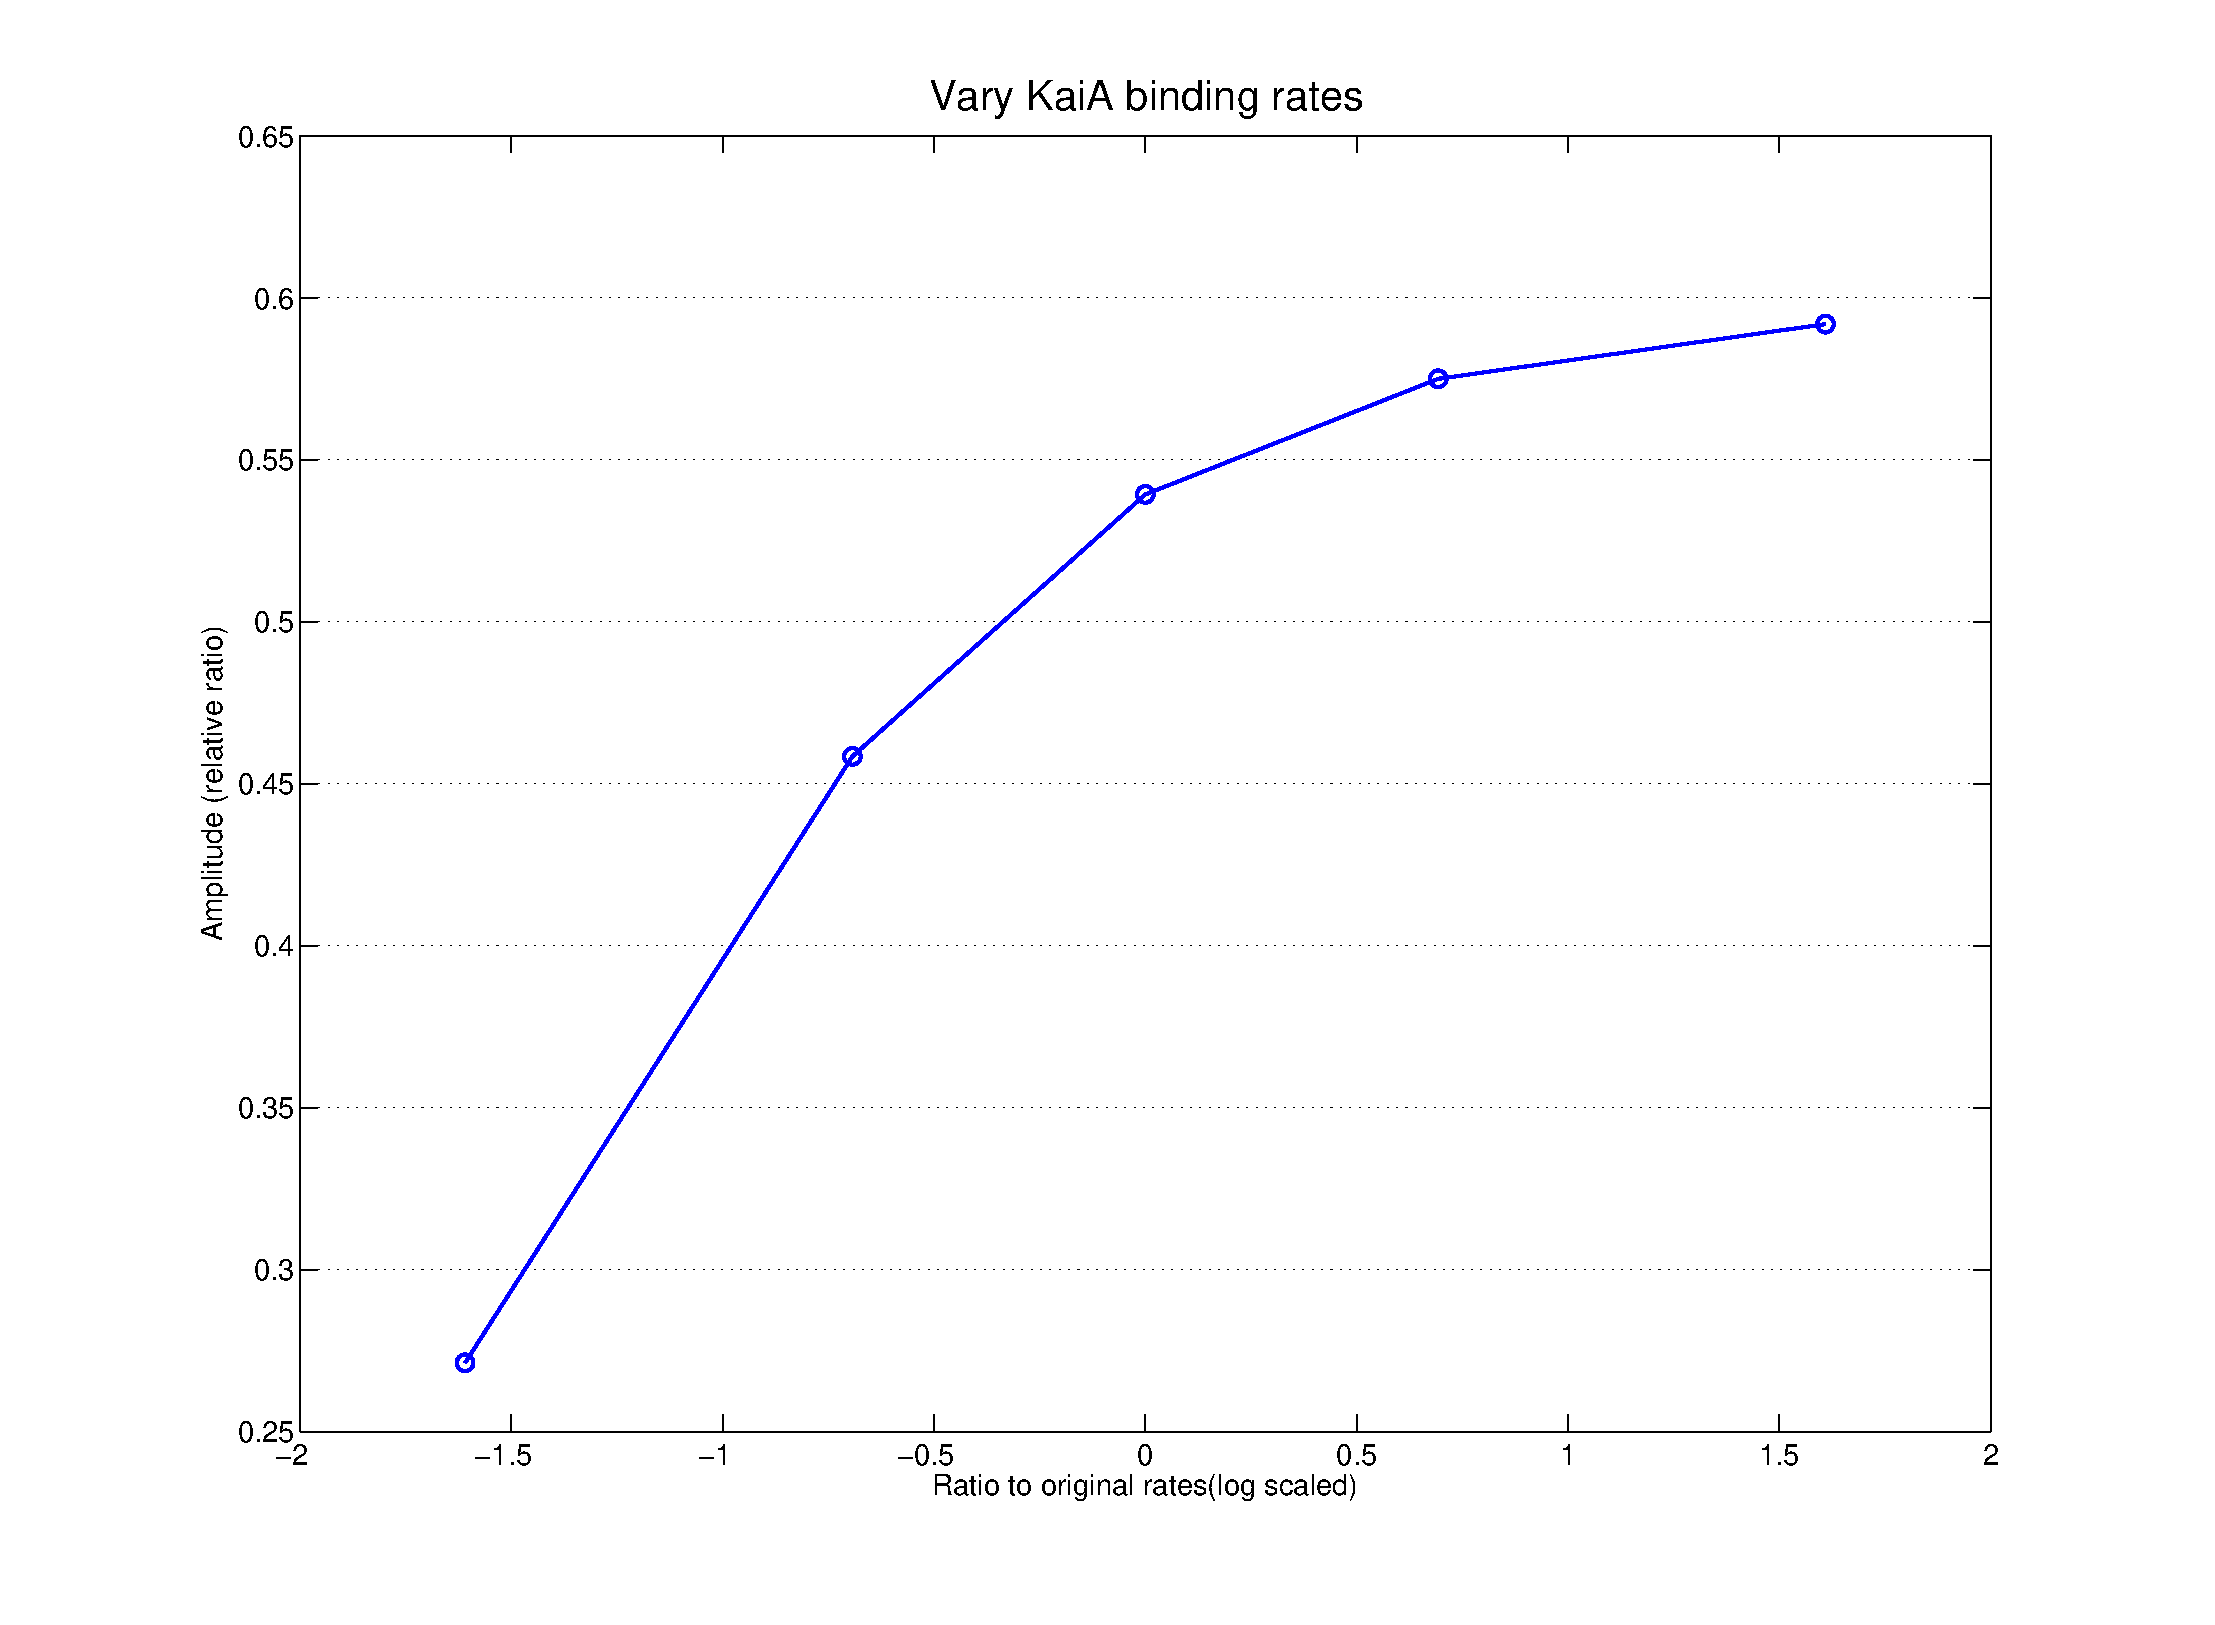
\includegraphics[scale=0.4]{tempcomp7.eps}
\caption{\fontfamily{lmss}\selectfont Amplitude increases as the reaction rates increases.}\label{fig:ampvary}
\end{figure}

% We therefore conclude that the KaiA-activated autokinase reaction can also serve as a temperature compensation element since when temperature is decreased, period is shortened while amplitude is decreased (Fig.\ref{fig:varycat} and Fig. \ref{fig:tempcomp8}). 

\begin{figure}[H]
\centering
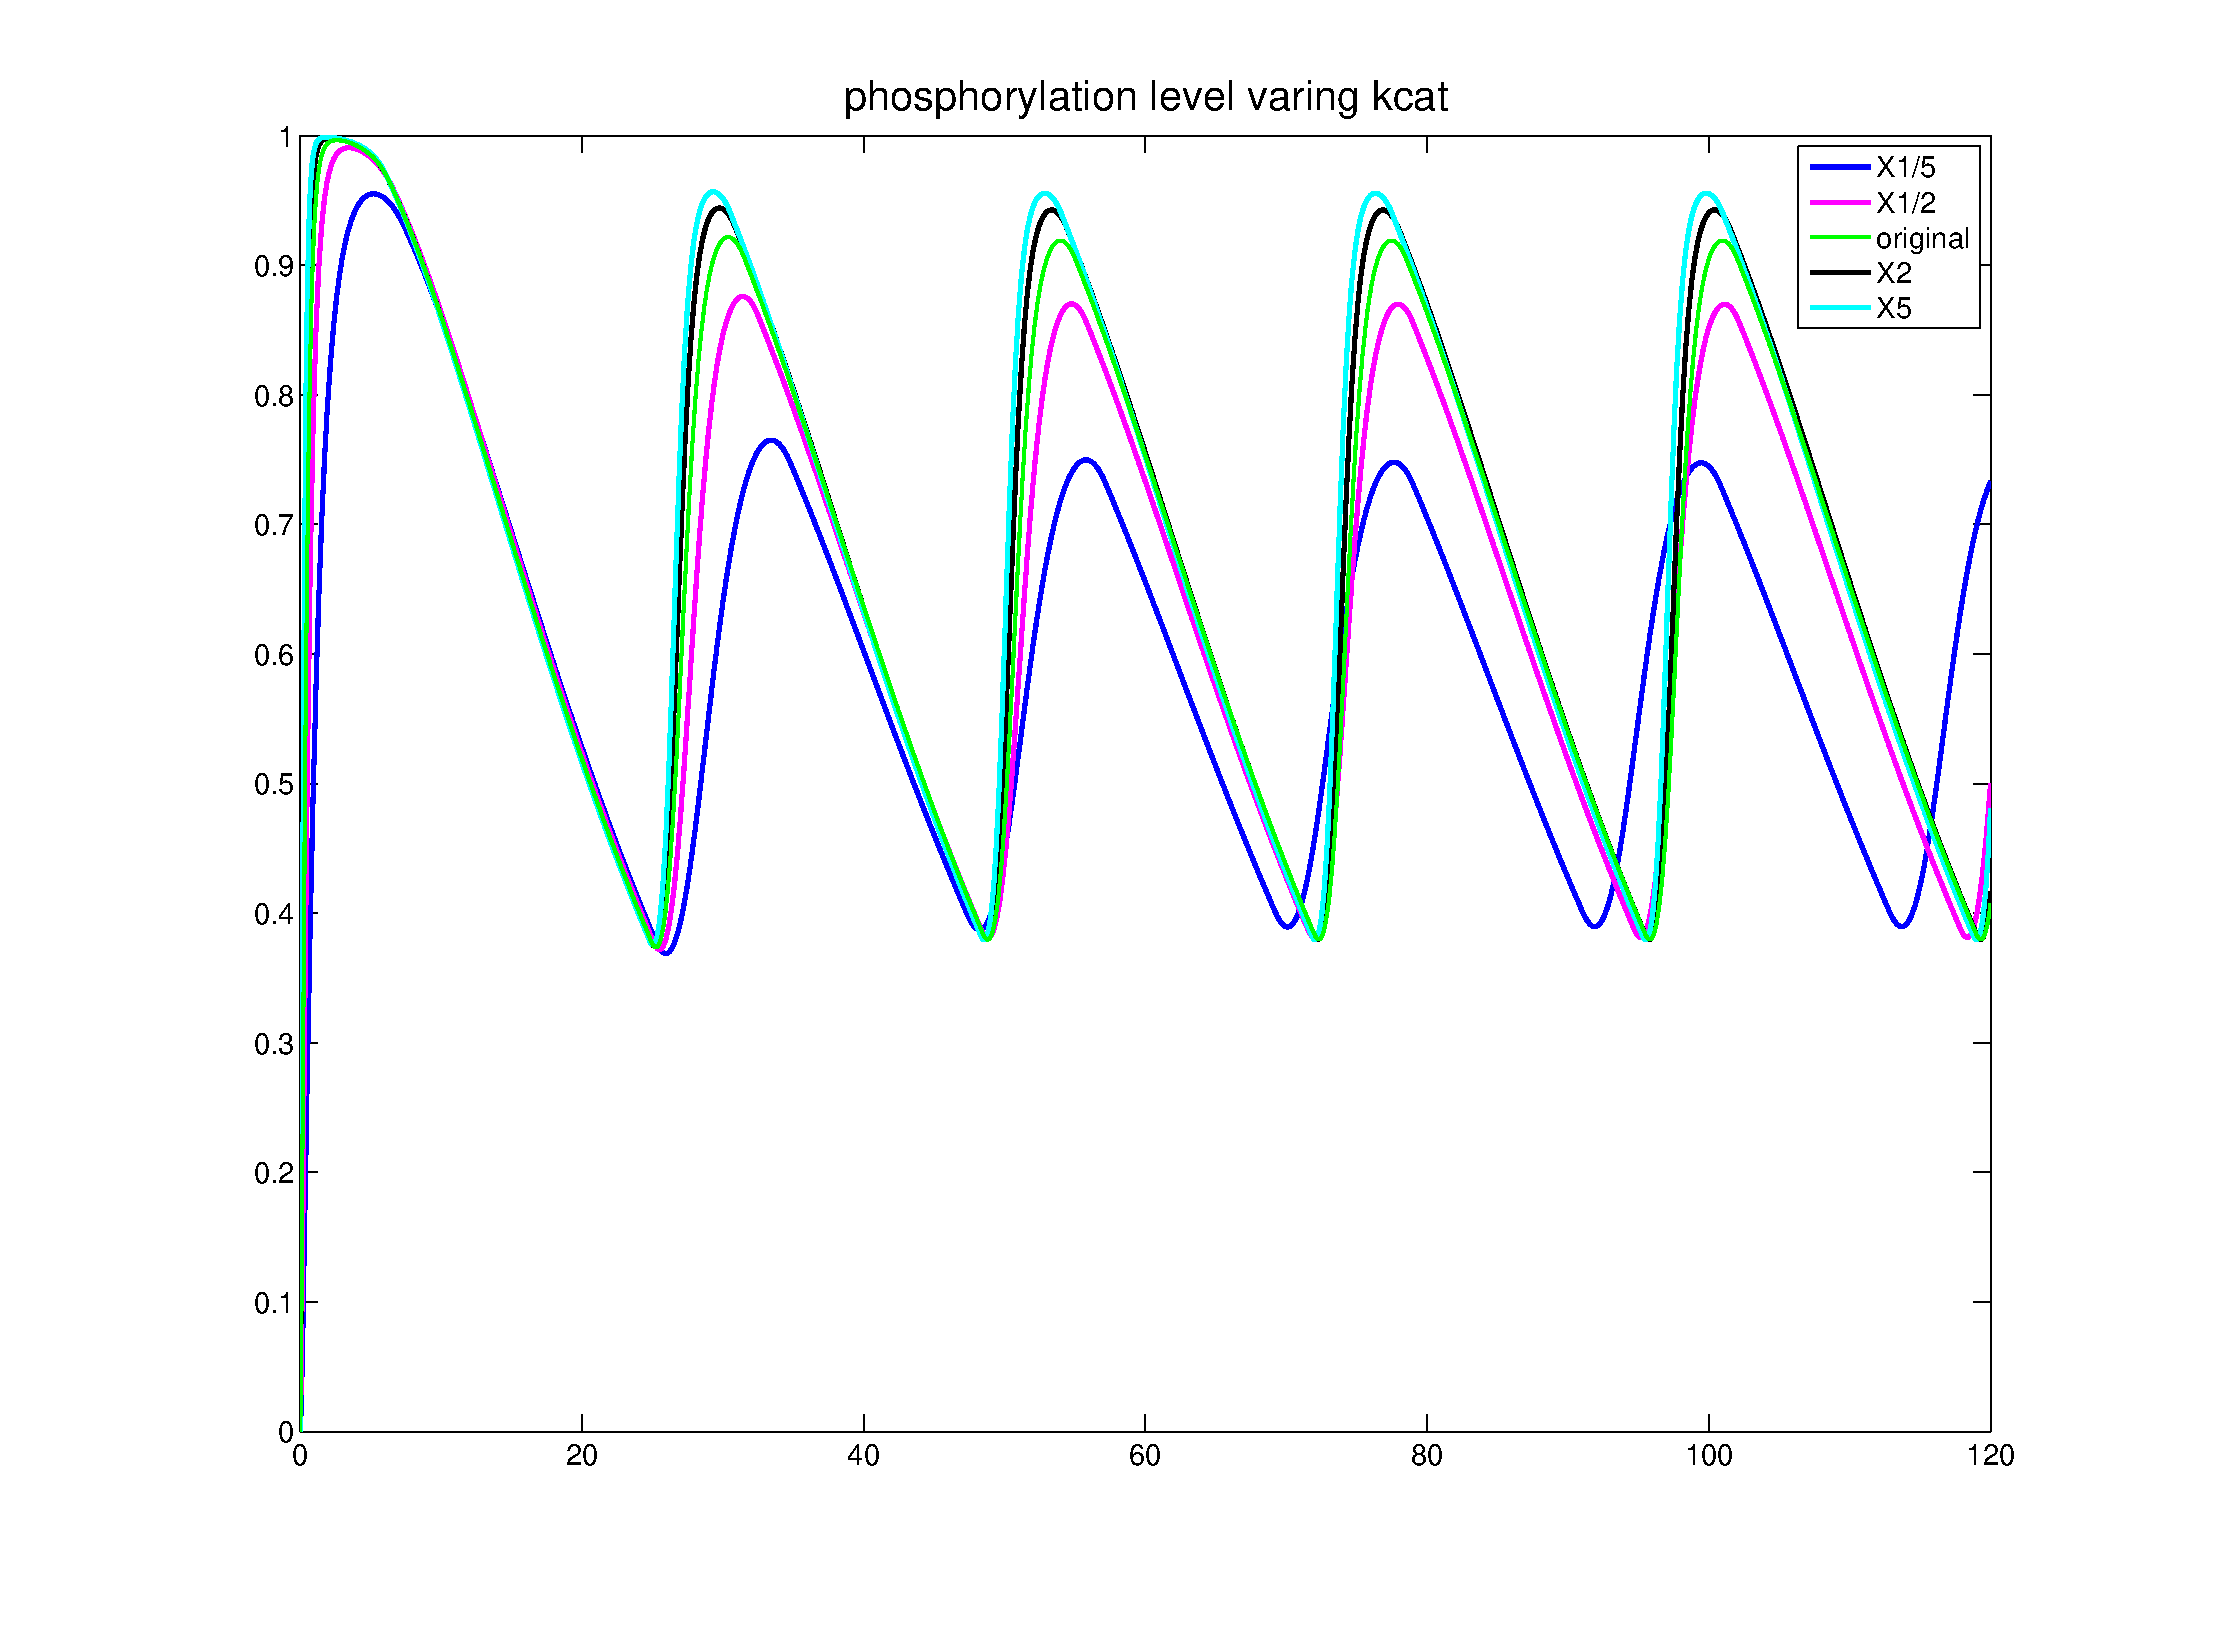
\includegraphics[scale=0.4]{tempcomp5.eps}
\caption{\fontfamily{lmss}\selectfont Different time profiles while varying KaiA-activated autokinase reaction rates.}
\label{fig:varycat}
\end{figure}

\begin{figure}[H]
\centering
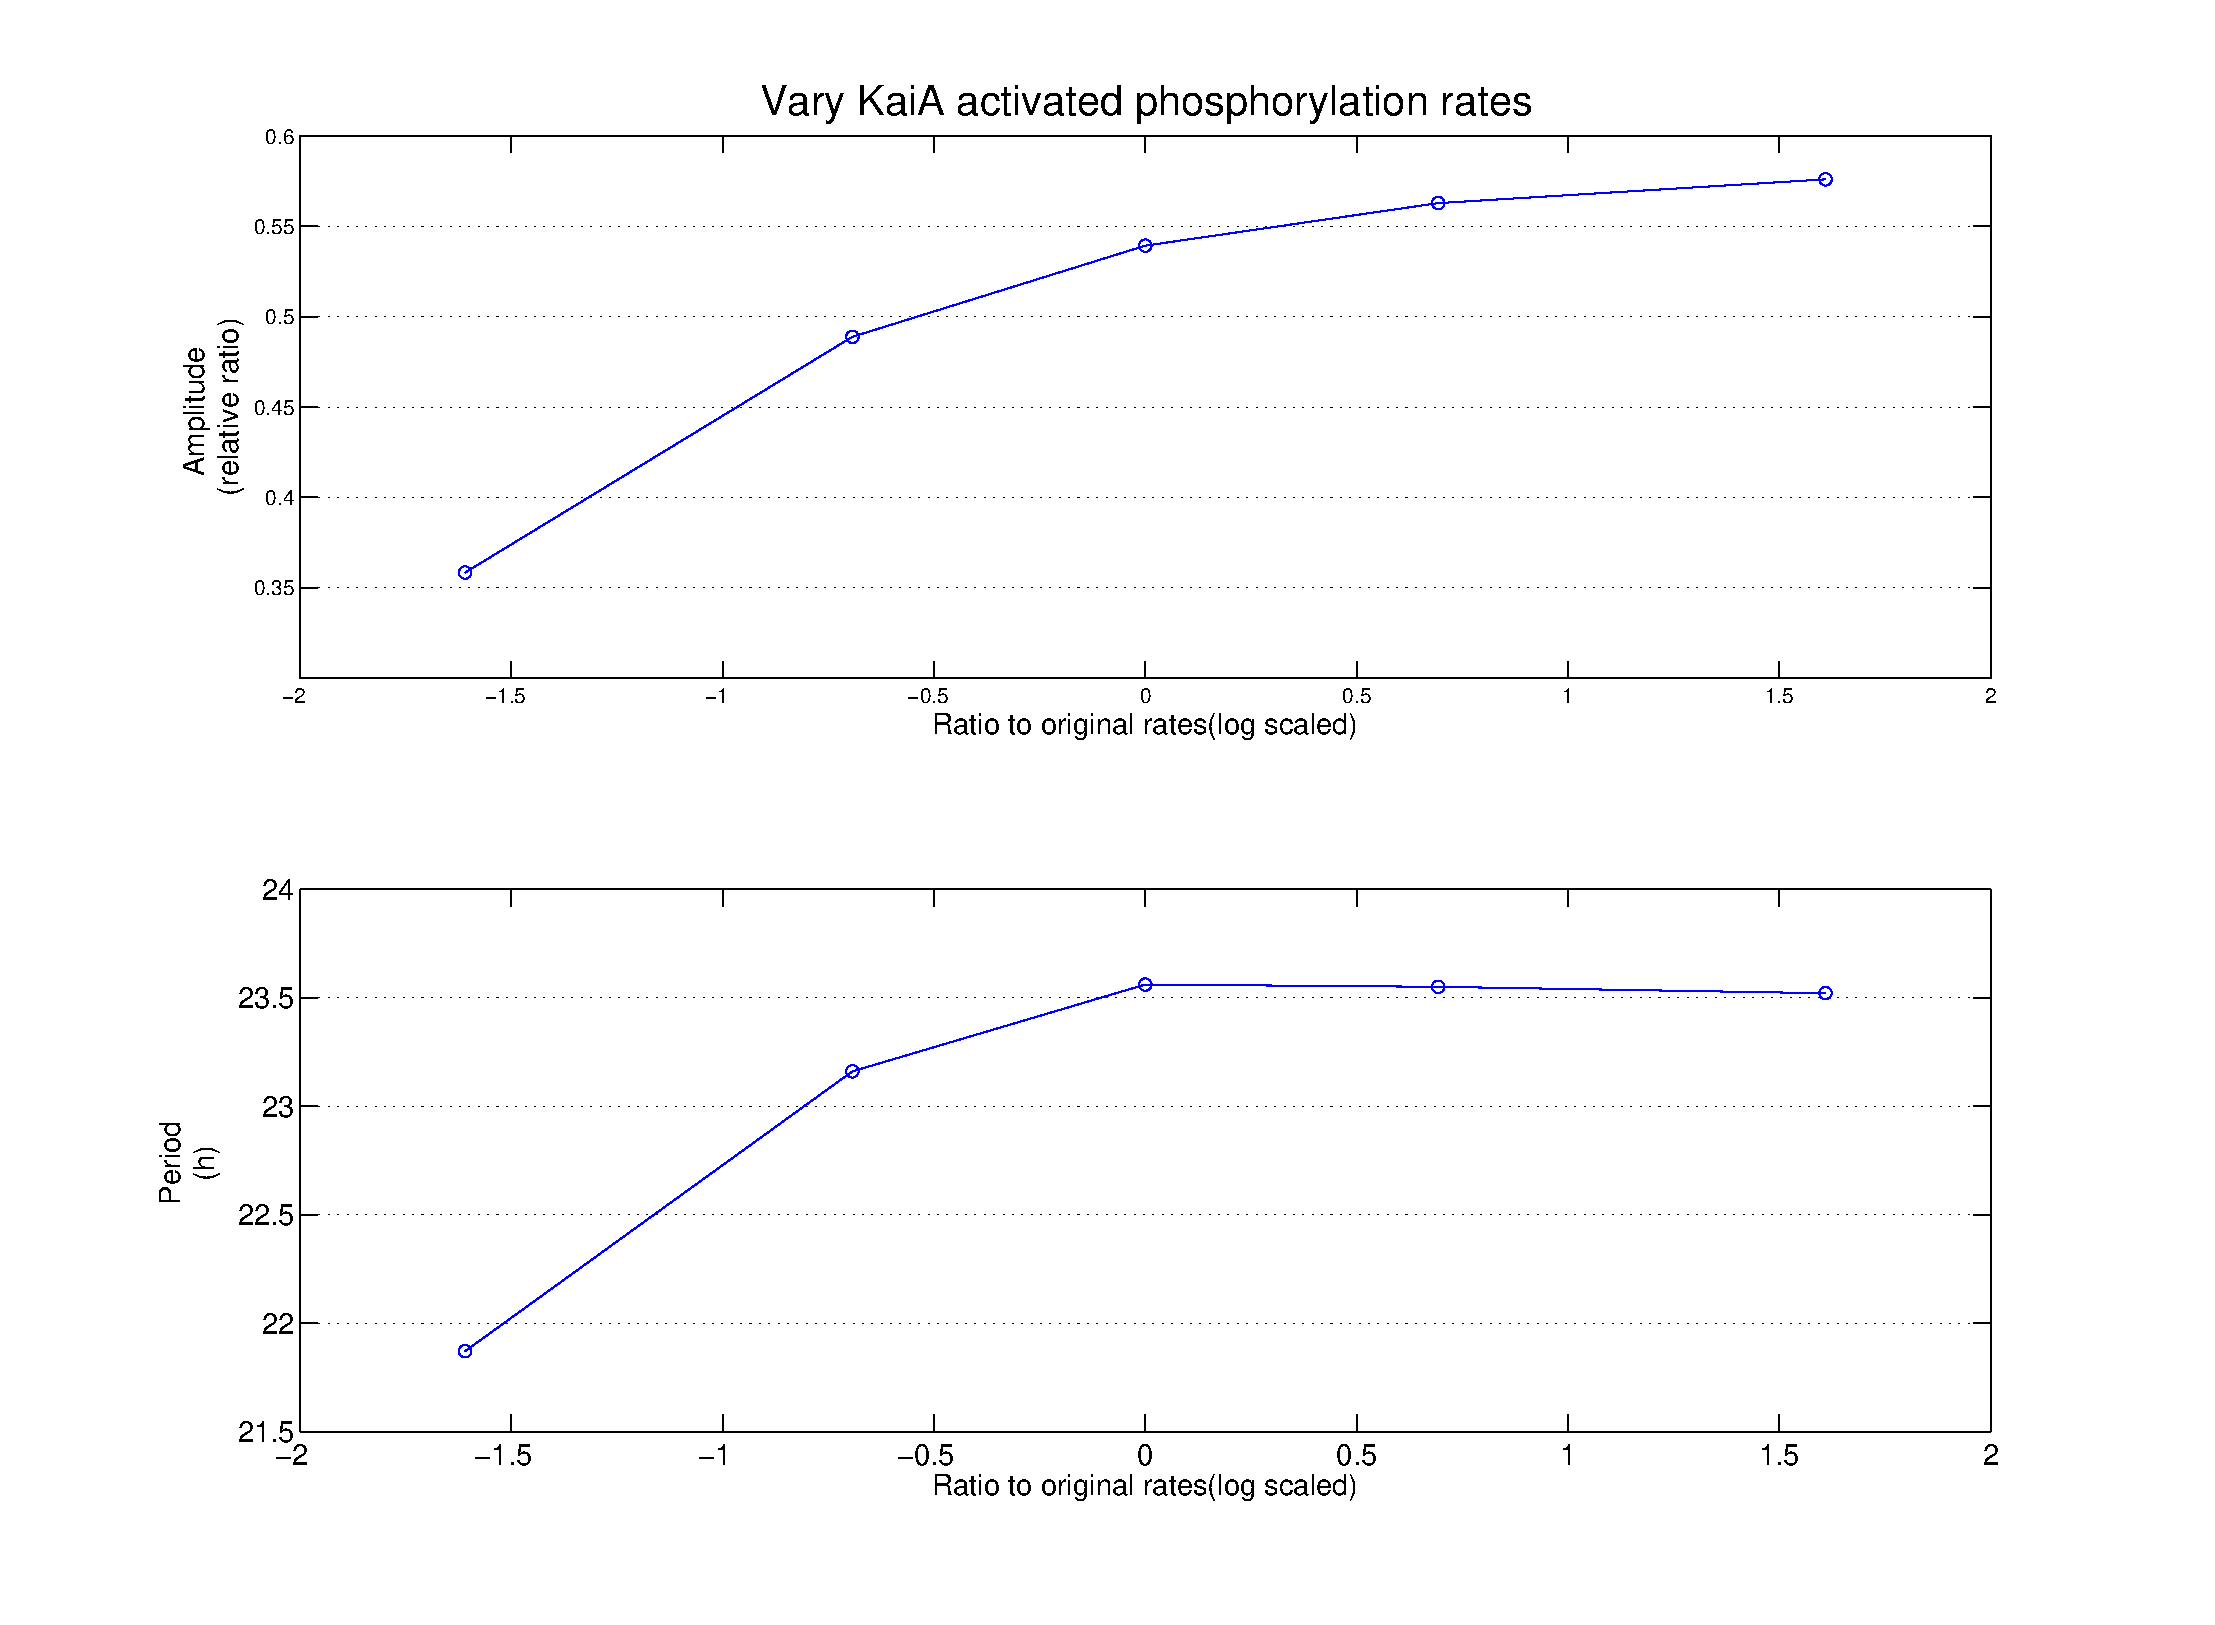
\includegraphics[scale=0.4]{tempcomp8.eps}
\caption{\fontfamily{lmss}\selectfont Period is optimized at a roughly 24h length. Lowering the rates by a factor 1/2 or 1/5 results in a shorter period. Amplitude increases as the reaction rates increases.}\label{fig:tempcomp8}
\end{figure}

\bibliography{review}
\end{document}